\documentclass[a4paper,11pt]{refrep}
\usepackage{color}

\usepackage{booktabs}
\usepackage{longtable}
\usepackage{rotating}
\usepackage{multicol}
\usepackage{multirow}
\usepackage[disable]{todonotes}
\usepackage[colorlinks=true]{hyperref}
\usepackage{gensymb}
\usepackage{makeidx}\makeindex
\makeatletter
\usepackage{fancyhdr}
\pagestyle{fancy}
\maxipagerulefalse
%
% Include XCSoar header and footer settings and used buttons 
% Add XCSoar User Manual title to the header
\fancyhead[RO,LE]{{\small \em XCSoar User Manual}}
\fancyhead[LO,RE]{}
\fancyfoot[RO,LE]{}
% Add page number to the footer (centered)
\fancyfoot[CO,CE]{\thepage}
% No line between content and header
\renewcommand{\headrulewidth}{0pt}

\fancypagestyle{plain}{
  % Clear fancy header and footer
  \fancyhf{}
  % Add page number to the footer (centered)
  \fancyfoot[CO,CE]{\thepage}
  % No line between content and header
  \renewcommand{\headrulewidth}{0pt}
}

\definecolor{buttongray}{rgb}{0.831,0.816,0.784}
\newcommand{\blink}[0]{$\triangleright$}
\newcommand{\bmenu}[1]{
	\fcolorbox {black}{buttongray}{{\sf{#1}}}
}
\newcommand{\bmenut}[2]{
	\fcolorbox {black}{buttongray}{
    \makebox[1.4cm][c]{
    	\begin{tabular}{c}
    	{\footnotesize\sf{#1}}\\
    	{\footnotesize\sf{#2}}
    	\end{tabular}
    }
  }
}
\newcommand{\bmenus}[1]{
	\fcolorbox {black}{buttongray}{
    \makebox[1.4cm][c]{
      \begin{tabular}{c}
        {\footnotesize\sf{#1}}\\
    	  \\
    	\end{tabular}
	  }
	}
}
\newcommand{\button}[1]{
	\fcolorbox {black}{buttongray}{{\sf #1}}
}

\newcommand{\infobox}[1]{
	\fcolorbox {black}{white}{\makebox[1.7cm][c]{\sf #1}}
}


\newenvironment{jspecs}{
\itemsep=2pt\topsep=3pt\partopsep=3pt\parskip=0pt
\begin{description}
\itemsep=2pt\topsep=3pt\partopsep=3pt\parskip=0pt
}
{\end{description}}

\newcommand{\jindent}[2]{
  \noindent\makebox[0pt][r]{{#1}\hspace*{\marginparsep}}
  \parbox[t]{0.95\linewidth}{#2}\par
}

%
\widowpenalty=1000
\clubpenalty=1000
%
%  XCSoar - Website Einfügen
\newcommand{\xcsoarwebsite}[1]{\url{http://www.xcsoar.org#1}}
%
% Define command to insert tip image
\newcommand{\tip}[0]{\marginlabel{\parbox{1.1cm}{
\includegraphics[width=0.7cm]{figures/reminder.pdf}}}}

% Define command to insert gesture image
\newcommand{\gesture}[1]{\marginlabel{{\it#1{\phantom{aa}}}\parbox{1.1cm}{\hspace{-3mm}
\includegraphics[width=0.8cm]{figures/gesture.pdf}}}}
%
% Define command to insert warning image
\newcommand{\warning}[0]{\marginlabel{\parbox{1.3cm}{
\includegraphics[width=0.9cm]{figures/warning.pdf}}}}
%
% Define command to insert Achtung image
\newcommand{\achtung}[0]{\marginlabel{\parbox{1.3cm}{
\includegraphics[width=2.5em]{figures/warning.pdf}}}}
%
% Define command to insert a flash image
\newcommand{\blitz}[0]{\marginlabel{\parbox{1.3cm}{
\includegraphics[height=2.0em]{figures/reminder.pdf}}}}
%
% Define command to insert a stop
\newcommand{\halt}[0]{\marginlabel{\parbox{1.3cm}{
\includegraphics[height=2.0em]{figures/warning.pdf}}}}
%
% Define command to reference a configuration item
\newcommand{\config}[1]{\marginlabel{\ref{conf:#1}\parbox{1.3cm}{
\includegraphics[width=0.8cm]{figures/config.pdf}}}}
%
% Potentially overdue ``InfoBox'' style macro but sometimes used... so ..let it be alive ..
\newcommand{\InfoBox}[0]{{InfoBox}}
%
% Define command to put a menu label on the margin
\newcommand{\menulabel}[1]{\marginpar{\parbox{5.0cm}{\raggedright #1}}}
%
% Define command to draw a sketch on the margin
\newcommand{\sketch}[1]{\marginpar{\parbox{4.750cm}{\includegraphics[angle=0,width=0.9\linewidth,keepaspectratio='true']{#1}}}}
%
% Define command to draw a small sketch on the margin
\newcommand{\smallsketch}[1]{\marginpar{\includegraphics[angle=0,keepaspectratio='true']{#1}}}
%
% Enumerated todo's for the todonotes package
\newcounter{todocounter}
\newcommand{\todonum}[2][]{\stepcounter{todocounter}\todo[#1]{\thetodocounter: #2}}
%
% dies nette Makro bringt mir die aktuelle Version der bearbeiteten XCSoar-Verrion aufs Papier 
\newcommand{\version}{\begingroup\catcode`\_=\active\input{VERSION.txt}\endgroup}
%
%Anführungszeichen per Tastatur einfach so eingeben -> "
\shorthandoff{"}%


% Set the title
\title{Podręcznik}

% Set the page title
% Add XCSoar User Manual title to the header
\fancyhead[RO,LE]{{\small \em XCSoar User Manual}}
\fancyhead[LO,RE]{}
\fancyfoot[RO,LE]{}
% Add page number to the footer (centered)
\fancyfoot[CO,CE]{\thepage}
% No line between content and header
\renewcommand{\headrulewidth}{0pt}

\fancypagestyle{plain}{
  % Clear fancy header and footer
  \fancyhf{}
  % Add page number to the footer (centered)
  \fancyfoot[CO,CE]{\thepage}
  % No line between content and header
  \renewcommand{\headrulewidth}{0pt}
}

\xcsoarheader{Podręcznik dla XCSoar}

% Define some xc doc styles
\def\maketitle{%
  \null
  \thispagestyle{empty}%
  \begin{maxipage}
  \begin{center}
  \includegraphics[angle=0,width=\textwidth,keepaspectratio='true']{xcsoar-title.png}
  \end{center}
  \begin{center}
    \normalfont\huge\textsf{Glide~Computer and Navigation~System}\par
  \end{center}
  \vskip 1cm
  \begin{center}
    \normalfont\huge\textsf{\@title}\par
  \end{center}
  \vskip 1cm

  \end{maxipage}
  \vfill
  \begin{flushright}
    \large \strut {\sf
\begin{tabular}{r}
Manual version 1.6 \\
\today \\
For XCSoar version 6.0 \\
\xcsoarwebsite \\
\end{tabular} } \par
  \end{flushright}
  \par
  \vfil
  \vfil
  \null
  \cleardoublepage
  }


% Select the right encoding and language package
\usepackage[polish]{babel}
\begin{document}

%%%%%%%%%%%%%%%%%%%%%%
% Front page
\maketitle

%%%%%%%%%%%%%%%%%%%%%%
% Todo's
\listoftodos
 
%%%%%%%%%%%%%%%%%%%%%%
% Table of contents
\begingroup
%\fontfamily{phv}
%\normalsize
%\fontseries{c}\selectfont
\setlength{\parskip}{0.05\baselineskip}
\makeatletter
\renewcommand*\l@section{\@dottedtocline{2}{1.3em}{2.6em}}
\makeatother
\tableofcontents
\endgroup


%%%%%%%%%%%%%%%%%%%%%%
\chapter*{Preface}

\section*{Warnings and precautions}

\warning IT IS THE USER'S RESPONSIBILITY TO USE THIS SOFT\-WARE PRUDENTLY. THIS SOFTWARE IS 
INTENDED TO BE USED ONLY AS A NAVIGATION AID AND MUST NOT BE USED FOR ANY PURPOSE REQUIRING 
PRECISE MEASURE\-MENT OF DIRECTION, DISTANCE, LOCATION, OR TOPO\-GRAPHY. THIS SOFTWARE SHOULD 
NOT BE USED AS AN AID TO DETERMINE GROUND PROXIMITY FOR AIRCRAFT NAVIGATION. THIS SOFTWARE 
SHOULD NOT BE USED AS A TRAFFIC COLLISION AVOIDANCE SYSTEM.


\section*{Legal notices}

\subsection*{Software license agreement}

This software is released according to the GNU General Public License
Version~2.  See Appendix~\ref{cha:gnu-general-public} for the full
text of the agreement and warranty notice.

\subsection*{Limited liability}

In no event shall XCSoar, or its principals, shareholders, officers,
employees, affiliates, contractors, subsidiaries, or parent
organizations, be liable for any incidental, consequential, or
punitive damages whatsoever relating to the use of the Product.

\subsection*{Disclaimer}

This product, and all accompanying files, data and materials, are
distributed "as is" and with no warranties of any kind, whether
express or implied.  This product is used entirely at the risk of the
user.  Although great care has been taken to eliminate defects during
its development it is not claimed to be fault-free. No claims are made
regarding its correctness, reliability or fitness for any particular
purpose.  The XCSoar project developers and contributors shall not be
liable for errors contained herein or for incidental or consequential
damages, loss of data or personal injury in connection with
furnishing, performance, or use of this material.


%%%%%%%%%%%%%%%%%%%%%%
\chapter{Introduction}\label{cha:introduction}
This document is a pilot's manual for XCSoar, an open-source glide
computer originally developed for Pocket PC devices.  The audience 
is assumed to have a sound knowledge of the fundamental theory of flight for
gliders, and at least a basic working knowledge of cross-country soaring.

Updates to the XCSoar software may result in some of this manual being
out of date. You should read the release notes distributed with the
software to keep track of changes.  Updates to the manual and software
are available from 
\begin{quote}
\xcsoarwebsite{}
\end{quote}

\section{Organization of this manual}

\todonum[inline]{Write about the manual crossref hinting icons and the yellow
colour. The Quickstart will be readable also without those links available} 
This manual most notably is written in order to get the XCSoar user started 
quickly  \emph{as well as} support his deep understanding of all the features, 
concepts and tactics introduced. At all times, the authors made their effort 
for doing this from a pilot's perspective (and honestly hope for having 
succeeded).

The authors highly encourage you to take your time reading the entire manual 
chapter by chapter (with exception of the reference chapters Infoboxes and 
Configuration). Feel assured, the time you will have spent will pay off as a 
manifold in understanding. On your way reading you might feel blue once in a 
while. That is why the authors introduced some blueish things: links and 
icons.

\begin{figure}[h]
\centering

\includegraphics[width=0.8cm,angle=0,keepaspectratio='true']{figures/config.pdf}
\hspace{1.5cm}

\includegraphics[width=0.8cm,angle=0,keepaspectratio='true']{figures/reminder.pdf}
\hspace{1.5cm}

\includegraphics[width=0.8cm,angle=0,keepaspectratio='true']{figures/gesture.pdf}
\hspace{1.5cm}

\includegraphics[width=0.8cm,angle=0,keepaspectratio='true']{figures/warning.pdf}
\caption{Icons configuration, reminder, gesture, warning}
\end{figure}

\warning Warning. The icon warning is used, whenever things shall be followed 
strictly.  Not following will cause unexpected results, total disfunction, or 
even danger to life. Proceed only, if warning understood.

\gesture{DU} Gesture. A swipe gesture input is available using devices with a 
touch screen to invoke a menu or function amongst others. In this example, DU 
stands for moving your fingertip down, then up, (in straight lines) on the 
screen.
  
\gesturespec{du} Specific Gesture. Whenever the manual's authors kept up with XCSoar's rapid development process
in writing, a specific icon is provided, depicting the movements.

\tip Reminder. This icon tags a tip, trick, things you might remind after having read corresponding sections and so on.

\config{orientation} Configuration see... The icon depicting two craftman's 
tools refers to an in-depth description of items being mentioned and how to 
configure them. The numbers beside the icon refer to a specific chapter / 
section of this manual's reference chapters \ref{cha:infobox} and 
\ref{cha:configuration}, in this case referring to section 
\ref{conf:orientation}. 

\marginlabel{\parbox{1.3cm}{\rotatebox[origin=c]{180}{
\includegraphics[width=0.9cm]{figures/warning.pdf}}}}
\rotatebox[origin=c]{180}{Stop from reading manuals whilst flying inverted!}

\emph{Read} at home, \emph{configure} on the ground, safely. Having perceived 
this (inverted) warning as an example, you are ready to proceed.

\config{usingxcsoarsafely} Referring to the second exemplary case of the icon 
"configuration" to the left, the icon points 
towards chapter \ref{cha:introduction}, (this chapter), section 
\ref{sec:usingxcsoarsafely}, "Using XCSoar safely" underneath, which could be 
understood as a "how to configure yourself". It is up to you whether to jump 
to an in depth discussion and go back or just proceed. If reading this manual 
electronically, clicking the number will let you jump to the requested cross
-reference.  Use the go-to "back" (or similar) function of your particular 
browser to proceed with the chapter you jumped from.

The numbers are printed in blue as are the icons introduced, signalling "help 
available". And so are other Universal Ressource Locators, underlaying blue 
text. Clicking on text like \xcsoarwebsite{/contact} will open your world wide 
web browser or mailer to get in touch with other ressources or konwledgeable 
people respectively.

The remainder of this chapter "Introduction" is about getting you prepared for 
XCSoar, how to raise your level of understanding and maintain your skills. 
Chapter \ref{cha:quickstart} "Quickstart" might be the next waypoint after 
\ref{cha:installation} "Installation" for the urgent user. Feel free to cut 
short, but do not resume too sadly when reading chapter by chapter, following:

Chapter~\ref{cha:interface} introduces the user interface
concepts and gives an overview of the display .

Chapter~\ref{cha:navigation} describes the moving map part of the
display in greater detail and describes how the software can assist in
general navigation.  Chapter~\ref{cha:tasks} describes how
cross-country tasks are specified and flown, and presents some of the
analysis tools available to pilots to help improve their performance.
Chapter~\ref{cha:glide} goes into further detail on the glide computer
functions as it is important for pilots to be aware of how the
computer performs its calculations.

Chapter~\ref{cha:atmosph} describes how the computer can interface to
variometers and other air data sensors, and how it uses these
measurements to provide various models of the atmosphere, in
particular on winds and thermal convection.
Chapter~\ref{cha:airspace} describes how XCSoar can assist in managing
flight in special use airspace and the FLARM collision awareness
system.  Chapter~\ref{cha:avionics-airframe} deals with systems
integration and systems diagnostics, the integration of XCSoar with
communications devices and with airframe switches.

The remainder of the manual contains mainly reference material.
Chapter~\ref{cha:infobox} lists the types of information that can be
displayed in the grid of InfoBoxes next to the map display.  The
configuration of the software is described in detail in
Chapter~\ref{cha:configuration}.  The formats of the various data
files that program uses, as well as where to obtain them from and how
to edit them, is described in Chapter~\ref{cha:data-files}.

Finally, a short history and discussion of XCSoar's development
process is presented in Chapter~\ref{cha:history-development}.

\section{Notes}

\subsection*{Screenshots}
Throughout this manual are several screenshots of XCSoar. These are
taken from the program running on a variety of hardware platforms and possibly
even different versions. Each platform and version may have different screen
resolutions, layouts and fonts, and so there may be slight differences in the
appearance of the display. Most of the screenshots in this manual are taken of
XCSoar running in landscape orientation.

\section{Platforms}
\begin{description}
\item[Android Devices]
XCSoar runs on Android 1.6 or newer.
\item [eBookreader]
XCSoar runs on some Kobo eReader devices. A native port has been released with version 6.7.1, but is still considered experimental (Nov. 2013).
\item[Windows PC]
It is possible to run XCSoar on an ordinary computer with the Windows
operating system. This setup can be used for training yourself in using XCSoar.
A simulation mode is included in XCSoar as well as a IGC replay function, that
can be used when not connected to a valid GPS source.
\item[Unix/Linux PC]
XCSoar can be run on Unix using the Wine emulator. A native Unix port
has been released with the 6.0 version of XCSoar, but is still
considered experimental.
\end{description}



\section{Technical support}

\subsection*{Troubleshooting}
A small team of dedicated developers produces XCSoar. Although we are
happy to help with the use of our software, we cannot teach you about
basics of modern information technology. If you have a question about XCSoar in
particular not found in this manual please get in touch. You will find all of the following links summarized at:
\begin{quote}
\xcsoarwebsite{/contact}
\end{quote}
To begin with communication, join the XCSoar forum at:
\begin{quote}
\url{http://forum.xcsoar.org}
\end{quote}
If your concern appears not already addressed, post it or email us: 
\begin{quote}
\href{mailto:xcsoar-user@lists.sourceforge.net}{xcsoar-user@lists.sourceforge.net}
\end{quote}
Any frequent questions will be added to this document and to the Frequently
Asked Questions (FAQ) section of the XCSoar website.
You may also find it useful to subscribe to the XCSoar users mailing
list so you will be kept up to date with latest developments.

If all of this does not help, you probably discovered a bug.

\subsection*{Feedback}
Like any complex software program, XCSoar may be subject to software
bugs, so if you find any, please report them to the XCSoar developers
by using our bug tracker portal at: 
\begin{quote}
\xcsoarwebsite{/trac}
\end{quote}
or by sending an email to
\begin{quote}
\href{mailto:xcsoar-devel@lists.sourceforge.net}{xcsoar-devel@lists.sourceforge.net}
\end{quote}
XCSoar logs many valuable things in a logfile
\verb|xcsoar.log| in the \texttt{XCSoarData} directory. The logfile can be appended to the bug ticket in order to help XCSoar developers determine the cause of possible problems.
If you like the idea of doing some more, get involved:
\begin{quote}
\xcsoarwebsite{/develop}
\end{quote}

\subsection*{Updates}
You should periodically visit the XCSoar website to check for program
updates. The installation procedure described above can typically be
repeated in order to upgrade the software.  All user configuration
settings and data files will be preserved during the
re-installation/upgrade.

It is also recommended to periodically check for updates to data
files, particularly Special Use Airspace, which may be subject to
change by the national civil aviation authority.

\section{Training}
For the safety of yourself and others, pilots using XCSoar are advised to
train themselves in using XCSoar on the ground and become familiar with its
interface and features prior to flight.

\subsection*{Using XCSoar on the PC}
The PC versions of XCSoar may be used to become familiar with XCSoar's
interface and functionality in the comfort of one's home.  All files
and configuration used by this version are identical to the embedded versions,
so it can be helpful to try out customisations on the PC version before using
them in flight.

The PC versions can also be connected to external devices and operate just as
the embedded versions do. Suggested uses include:
\begin{itemize}
\item Connect the PC to a FLARM device to use XCSoar as a ground
station display of FLARM-equipped traffic.
\item Connect the PC to an intelligent variometer such as Vega to
test configuration settings of the variometer.
\end{itemize}

\subsection*{Using XCSoar with a flight simulator}
A good way to learn how to use XCSoar is to connect the Pocket PC
device to a PC running a flight simulator that can output NMEA
sentences to the serial port. Suitable simulators include Condor and
X-Plane.  

The benefit of this form of training is that XCSoar can be used in FLY
mode, so it behaves exactly as if you were really flying, and you can
get a good feel for how the program works while you are flying the
simulator.

\section{Using XCSoar safely}\label{sec:usingxcsoarsafely}\label{conf:usingxcsoarsafely}
The use of an interactive system like XCSoar in flight carries with it
certain risks due to the potential distraction of the pilot from
maintaining situational awareness and eyes outside the cockpit.

The philosophy guiding the design and development of the software is
to try to reduce this distraction by minimising the need for user
interactions as much as possible, and by presenting information in a
clear fashion able to be interpreted at a glance.

Pilots using XCSoar must take responsibility for using the system safely.
Good practice in the use of XCSoar includes:
\begin{itemize}
\item Becoming familiar with the system thoroughly through training on 
  the ground.
\item Performing clearing turns before interacting with XCSoar in flight
  in order to ensure there is no collision risk with other traffic.
\item Setting up the system to take advantage of automatic functions
  and input events so that user interactions can be minimised.  If you
  find yourself mechanically performing certain interactions frequently,
  ask yourself (or other XCSoar users) if the software can be made to do 
  these interactions for you.
\end{itemize}

\chapter{Installation}\label{cha:installation}

To run XCSoar, you need to obtain the following:

\begin{itemize}
\item a device to run XCSoar on
\item XCSoar
\item a GPS receiver
\item a waypoint file
\item an airspace file (optional)
\item a map file (optional)
\end{itemize}

\section{Compatibility}

\subsection{Devices for running XCSoar}

XCSoar runs on the following platforms:

\begin{itemize}
\item mobile phones and tablets with Android 1.6 or newer \\
  Example: Dell Streak, Samsung Galaxy S II, HTC Desire HD,
  Motorola Xoom
\item PDAs with Pocket PC 2000, 2002, 2003 \\
  Example: iPaq 3800, iPaq 3900
\item PDAs with Windows Mobile \\
  Example: iPaq hx4700, Dell Axim x51v
\item PNAs with Windows CE 3.0 or newer \\
  Example: HP314, Mio400
\item Triadis Altair
\item LX MiniMap
\item Windows 2000 or newer
\item Linux
\end{itemize}

\subsection{GPS, Logger, Vario}

XCSoar is compatible with any GPS emitting NMEA data.  Most modern
Android devices have a built-in GPS, but sometimes it is favorable to
connect to an external device:

\begin{itemize}
\item an airspeed indicator allows quick and exact wind estimates
\item a vario improves the thermal assistant
\item a task can be declared to an IGC logger, and after landing, the
  flight log can be downloaded
\item some varios allow synchronising the MacCready setting with
  XCSoar
\end{itemize}

\begin{figure}
\begin{tabular}{l|cccc}

Product & Airspeed & Vario & Declaration & Download \\

\hline

Borgelt B50 & $\surd$ \\

CAI 302 & $\surd$ & $\surd$ & $\surd$ & $\surd$ \\

CAI GPS Nav \\

Condor & $\surd$ \\

Digifly Leonardo & $\surd$ & $\surd$ \\

EW Logger &&& $\surd$ \\

EW microRecorder &&& $\surd$ \\

Flymaster F1 && $\surd$ \\

Flytec 5030 & $\surd$ & $\surd$ \\

ILEC SN10 & & $\surd$ \\

IMI ERIXX &&& $\surd$ & $\surd$ \\

LX20, Colibri &&& $\surd$ & $\surd$ \\

LX 5000, 7000 & $\surd$ & $\surd$ & $\surd$ \\

PosiGraph &&& $\surd$ \\

Triadis Altair &&& $\surd$ \\

Triadis Vega & $\surd$ & $\surd$ \\

Volkslogger &&& $\surd$ \\

Westerboer VW1150 & $\surd$ & $\surd$ \\

Zander / SDI & $\surd$ & $\surd$ \\

\end{tabular}
\caption{Supported external devices and some of their features}
\end{figure}

While most Windows CE based devices have a serial port, such legacy
hardware is not present in modern Android devices.  Those can either
use Bluetooth or the Android IOIO board.  To use Bluetooth, you need
to connect the external device to a Bluetooth-to-Serial adapter, such
as the K6-Bt or the Glidertools VFBT-1.

\section{Downloading XCSoar}
The software is available as a free download from the XCSoar website
~\xcsoarwebsite. Follow the links to the download section.

\subsection*{Pocket PC versions}
Download the relevant package for your Pocket PC operating system
version and save it to disk:
\begin{description}
\item[Pocket PC 2000] For Pocket PC 2002 and older
\item[Windows Mobile 2003] For Windows Mobile 2003 (or Pocket PC 2003)
\item[Windows Mobile 5] For Windows Mobile 5 and 6
\end{description}

\subsection*{Data files location}
To be able to use XCSoar's advanced features, additional data files, such as
terrain, topography, special use airspace, waypoints etc.\ are needed. The files
that can be used with XCSoar are described in Chapter~\ref{cha:data-files}.

All data files should be copied into the directory
\texttt{XCSoarData}.  This directory must be in a specific place
so that XCSoar knows where to look for data files:

\begin{description}
\item[Windows PC]
\texttt{XCSoarData} must be located in your personal folder (``\texttt{My
Documents}'')
\item[Windows Mobile PDA/PNA]
\begin{itemize}
\item If you start XCSoar from a SD card, it is always in the root of
  that SD card (e.g. ``\texttt{SD Card/XCSoarData}'')
\item If \texttt{XCSoarData} already exists on any SD card inserted
  at XCSoar start\-up, this one is used.
\item If none of the above applies, then it is in your personal folder
  (``\texttt{My Documents/}'')
\end{itemize}
\item[Unix PC]
\verb|~/.xcsoar/XCSoarData|.
\item[Android Devices]
\texttt{XCSoarData} is located on the SD card (e.g.
``\texttt{/sdcard/XCSoarData}'').
\item[Altair]
If XCSoarData exists on an USB drive, that one is used, otherwise the
internal storage is used.
\end{description}

For embedded devices it is recommended to create \texttt{XCSoarData} on a SD
card, because you can easily update the data files using your PC.


XCSoar will generate a number of additional files at run time.  These
will be placed in the  \texttt{XCSoarData} directory (Windows PC and 
Windows Mobile devices), or the \texttt{.xcsoar} directory (Unix/Linux
PC).  At first run, XCSoar will create the files 
\texttt{Default.tsk} (Default Task),  \texttt{xcsoar-registry.prf} 
(configuration settings), \newline
\texttt{xcsoar-startup.log} (log of the startup progress), 
plus three directories: \texttt{cache},
\texttt{config} and \texttt{logs}.  Additional files may be
created/modified while XCSoar is running, such as task files
(\texttt{*.tsk}) and flight logs.




\section{Installation}

\subsection*{Installation of Pocket PC version from a Pocket PC CAB file}

You can download the CAB file appropriate for your organiser and
install it onto a nonvolatile storage card like a Compact Flash or
Secure Digital card. Place it in your organiser. Use the File Manager
on your organiser to find the CAB and click on it to execute
it. Follow the on-screen instructions, the CAB file will be deleted
after installation.

Alternatively you can download the CAB file from Sourceforge through
your Internet Explorer on your organiser and install it that way.

After the installation, the XCSoar `FLY' and `SIM' launcher icons will
be visible on the Today screen.

\begin{center}
\includegraphics[angle=0,width=0.6\linewidth,keepaspectratio='true']{figures/XCS_Today.png}
\end{center}

\tip It is generally a good idea to keep the CAB file on the storage card
so that if the organiser's power fails and the memory is lost, XCSoar
can be reinstalled.

\subsection*{Installation of PC version}

The file \verb|XCSoarPC.zip| needs to be unzipped using a utility
program such as WinZip.

Development of a proper windows installer for the PC version is in
progress.  For now, any additional data files used by the PC version
must be placed in the \verb|My Documents\XCSoarData| directory.


\subsection*{Installation on Unix/Linux}

The file downloaded is \verb|xcsoar_XXX.deb|, where \verb|XXX| includes
the version number and platform, e.g. \verb|xcsoar_6.0.4_i386.deb|.
The is a Debian package and can be installed using 
\begin{center}
\verb|sudo dpkg -i xcsoar_XXX.deb|.
\end{center}
Use \verb|dpkg-query -L xcsoar| to see where the executable and 
other files are installed,
Additional data files must be placed in the directory
\verb|~/.xcsoar/XCSoarData/|.
If \verb|~/.xcsoar| does not exist, it will be created the first time
that \verb|xcsoar| is run.


\subsection*{Installation on Android}

Obtain XCSoar from Google's Android market, or install the \verb|apk|
file manually.  Copy the data files on the SD card in the directory
\verb|XCSoarData|.


\section{Running XCSoar}
%\subsection*{Fly and simulator modes}

Two modes are available inside the XCSoar application: 
\begin{description}
\item[FLY] This mode is used when actually flying.  The simulator is 
  disabled and serial communications are active. 
\item[SIM] This starts XCSoar in simulator mode, no serial communications
  are attempted.
\end{description}

\subsection*{XCSoar Pocket PC version}
The program can be run in either of two modes by pressing the `FLY' or
`SIM' launcher on the Today screen. If the application is started directly from
the explorer a dialog is asking you which mode you want to start.

\tip It is recommended that on Pocket PC devices, no other programs
 are running while XCSoar is used in flights.  This gives the best
 possible performance and responsiveness of the program.

\subsection*{Altair version}
XCSoar starts up automatically when Altair is powered on.
The PWR/ESC button (top left) has multiple functions:
\begin{description}
\item[Powering on]  Press and hold the PWR/ESC button for one second.
  The LED in the button will light up, and XCSoar will start after
  Altair has booted.
\item[Powering off]  Press and hold the PWR/ESC button for 3 seconds.
  Altair will switch off.
\item[Escape] Pressing the PWR/ESC button quickly acts as an
Escape key, typically used to close dialog pages or as a cancel function.
\end{description}

The Altair version of XCSoar does not include a simulator mode.

\subsection*{XCSoar PC version}
The program can be run by opening the explorer window, finding the directory
that has the XCSoar.exe executable, and double clicking on that program file.

The program command line options allows the screen orientation of
the display to be defined:
\begin{description}
\item[-portrait] The screen is 480 pixels wide, 640 pixels high.
\item[-square] The screen is 480 pixels wide, 480 pixels high.
\item[-landscape] The screen is 640 pixels wide, 480 pixels high. This is the
usual setting. If you don't specify this parameter the landscape version will be
loaded automatically.
\item[-small] Draws the screen at half size.  This is useful for using XCSoar in
 conjunction with flight simulators e.g.\ Condor.
\end{description}
To change the screen orientation, it is convenient to create a shortcut to the
program, then right click on the shortcut icon and click on ``Shortcut''. 
In the field ``Target'' add one of the desired options listed above.

\subsection*{XCSoar Unix/Linux PC version}
Run \verb|xcsoar| from a command line, or create a shortcut on the
desktop.  The location of the executable file may be found using
\verb|which xcsoar|.  Only landscape mode is  supported for now.

\subsection*{Loading data files}
The first time that XCSoar is run, it does not automatically load the 
data files that you placed in the \verb|XCSoarData| directory.  
To tell XCSoar which files to load, double click/tap the map (the large,
blank white part with the glider symbol in the center),
choose the menu \bmenu{Config} (click/tap it twice), then select
\bmenu{System Setup}.  The System Setup screen should be displayed:
\begin{center}
\includegraphics[angle=0,width=0.8\linewidth,keepaspectratio='true']{figures/config-basic.png}
\end{center}
The first page allows you to choose the map, 
waypoint and airspace files, by clicking/tapping on the text boxes.
Many other features of XCSoar may be configured with
\bmenu{System Setup}. These are described in detail in Chapter
\ref{cha:configuration}.
Once completed, XCSoar must be restarted; from now on, the data files
will be loaded automatically at run time.

\subsection*{Start-up and user profiles}
When XCSoar starts up, it will check for existing profiles. If multiple
profiles are detected it will displays a small window asking you which profile
to load. To proceed, choose the desired profile and press Enter. If no
profile is chosen the settings from the last session are loaded again. Profiles
can be useful for example in the following cases:
\begin{itemize}
\item Different pilots
\item Competition versus casual flying
\item Flying in different locations
\end{itemize}


\subsection*{SIM mode}
The simulator contains a simple interface allowing the user to fly
the glider about.  On the map screen, clicking/touching the glider symbol
(with touchscreen or mouse) and dragging 
causes the glider to move in the direction of the drag, the
speed being proportional to the length of the drag.  

In the PC version and for embedded devices with buttons, the aircraft
speed, height and direction may be changed using the \InfoBox es.
These features are not available for touchscreen devices.
The aircraft altitude can be adjusted by selecting the GPS altitude
{\InfoBox} (marked \infobox{H GPS}), and pressing the up or down key.
The airspeed  can be adjusted by selecting the ground speed
{\InfoBox} (marked \infobox{V Gnd}), and pressing the up or down key.
The glider's track  can be adjusted by selecting the track
{\InfoBox} (marked \infobox{Track}), and pressing the up or down key.
With either of the \InfoBox es \infobox{H GPS} or \infobox{V Gnd})
selected, the glider's direction may be changed using the left/right keys.

Other controls, buttons and menus work the same as in FLY mode.


\subsection*{Splash screen}
When XCSoar starts up, shuts down, or loads large files, such as airspace,
waypoints, terrain, etc., a progress screen is presented while the data is being
loaded. This screen has a progress bar which indicates the data loading
activity, and a short line of text describing the action that is being performed.

This screen also displays the software version information.

\subsection*{Exiting the program}
For PDA and PC versions, XCSoar is shut down from the menu. The menu can be
opened by double-clicking on the map or the \InfoBox es.
\begin{quote}
\bmenu{QUIT}
\end{quote}

For PC versions, XCSoar can also be shut down by clicking the close icon
on the XCSoar window.

For Altair, XCSoar is shut down by holding the PWR button for two seconds or
more.



%%%%%%%%%%%%%%%%%%%%%%
\chapter{User Interface}\label{cha:interface}
This chapter describes the fundamental user interface concepts used by
XCSoar, and is intended as an overview.  More detailed descriptions
are given in following chapters.

\begin{center}
\includegraphics[angle=0,width=\linewidth,keepaspectratio='true']{figures/plain.png}
\end{center}

The XCSoar display is composed of several parts:
\begin{description}
\item[Map area] The bulk of the screen is dedicated to the GPS moving map
display. Various symbols relating to glide computer information are overlaid 
on the map area. Icons and text may appear along the lower edge of the screen
to indicate status of connected devices, operating modes etc.
\item[InfoBoxes] A grid of data values is displayed usually either along
the top and bottom of the screen (portrait display) or to the right of the
screen (landscape display).  These so-called InfoBoxes display data from the
GPS and other input devices as well as data calculated by XCSoar.
\item[Gauges]  Gauges provide instrumentation displays. All gauges are optional
and some may only have meaningful information displayed when XCSoar is
connected to a supported instrument.
\item[Button labels and menus] Hardware buttons on the device running XCSoar
can be used to bring up and navigate smaller on-screen menus that are
typically laid out such that menu items can be selected by pressing the
button adjacent to the item.  If the device has a touch screen, the menu
items can be selected by touching them.  These buttons are drawn in black
text on a grey background.
\item[Status messages] Text is displayed over the map area in status message
boxes.  This text is used to present detailed information to the pilot when
certain events occur.
\item[Dialogue windows] Larger dialogue windows, usually containing graphics and
buttons, are used to present detailed data to the pilot regarding waypoint
details, statistics and analysis etc.
\item[Main menu] The main menu is accessible by double tapping the map area or
InfoBoxes as well as through gesture\gesture{Down - Up}. If the menu buttons are
not pressed after a specified time, they disappear again so as to not obscure the map area.
\end{description}

There are several ways to interact with XCSoar:
\begin{itemize}
\item Touching certain map elements
\item Touching InfoBoxes and on-screen menu buttons
\item `Gesturing', by e.g. drawing a dash from the left to the right
  on the screen (see Section \ref{sec:gestures} below).
\item `Dragging' the screen (touching the screen and moving before releasing).
\item Pressing application buttons on the device.
\item Pressing the cursor keys on the device.
\item Pressing keys or switches on an instrument connected to XCSoar.
\end{itemize}
Depending on the particular hardware used with XCSoar, not all of these methods
of interaction are possible and there may be different numbers or assignments
of buttons.

For the PC version of XCSoar, clicking the mouse over an item is equivalent to
touching it.

Since the Altair does not have a touch screen, all user interaction is performed
via physical buttons, switches or other external interface devices if connected.

\section{The main button menu}
The button menu is a set of buttons drawn on the screen and activated by touch
or hardware button presses.  Using buttons and the button menu is the primary
way the user interacts with XCSoar.

\subsection*{Interface basics}
The menu is organised into four different groups of functions, usually in
the form of a hierarchy.  The specific menu layout depends on the
hardware button configurations and platform, and may also be customised by the
user.

XCSoar can also accept input from external keyboards, game-pads, joysticks,
stick grip switches etc. A wide variety of functions can be assigned to these
inputs.
\sketch{figures/buttonmenu.png}

For Altair, there are four major menus, activated by pressing one of
the vertical strip of hardware buttons on the left of the display.
When a menu is activated, a strip of on-screen buttons appear along the 
bottom of the display.  Pressing the particular menu button again will
cycle through several pages of items.  Pressing the corresponding
horizontal button will activate that item.  At the last page, pressing
the menu button again will turn that menu off and the horizontal strip
of on-screen buttons disappear.  

On the PC version, these mode buttons are activated by the
1, 2, 3 and 4 keys.  The 6, 7, 8, 9 and 0 keys correspond to the horizontal
strip of buttons.

On the PDA version, the mode buttons are activated by the keys to the
side of the joystick/rocker button.

If the user doesn't interact with the computer for some time, the
menu will close automatically.  This menu time-out is configurable.
The escape key on PC, or the PWR/ESC button on Altair, can
also be used to close the current menu.

Menu buttons appear greyed out if the corresponding function is not available. 
For example, the ``Waypoint list'' function will appear grey if there are no waypoints loaded.

Several menu button labels have dynamic text based on context, in
order to make it clearer as to what happens when the button is
pressed.  The convention is used that a button's label describes what
will happen when the button is pressed.  For example, if the button
says \bmenu{MC Auto}, then pressing the button will turn on `Auto
MacCready', and the button label will then change to \bmenu{MC Manual}. 
In the menu list described below, generic labels are used.

\subsection*{Menu function groups}
This section describes the default layout of the menu system on all
platforms.  The functions performed by each button are explained more
fully in following chapters.

The primary menu buttons are activated by each of the vertical strip of buttons
on Altair, from top to bottom:
\begin{jspecs}
\item[\bmenu{Nav}] Actions for navigation control, primarily cross-country
gliding tasks.
\item[\bmenu{Display}] Actions to control the display.
\item[\bmenu{Config}] Configuration of XCSoar, connected devices, and in-flight
settings.
\item[\bmenu{Info}] Activates various informational dialogue windows.
\end{jspecs}

For the PC version, the keys 1, 2, 3 and 4 activate the 
corresponding menu.  The following menu item list has on the left side of most 
of the menu buttons links to the respective section. Follow them to get to all 
related details.

\section{Menu item overview}

\subsection*{Navigation menu}
\noindent\makebox[\textwidth]{%
\begin{tabularx}{1.8\textwidth}{l|ccccc}

Nav 1 & \ref{cha:tasks}\bmenus{Task}
 & {\bmenut{Previous}{Turnpoint}} & {\bmenut{Next}{Turnpoint}}
 & \ref{sec:waypoint-selector-dialog}\bmenut{Waypoint}{List}
 & \ref{sec:alternates}\bmenus{Alternates} \\ \\
Nav 2 & \ref{sec:taskabort}\bmenut{Task}{Abort}
 & \ref{sec:markers}\bmenut{Mark}{Drop}
 & {}
 & \bmenus{Target}
 & \ref{sec:waypointdetails}\bmenut{Waypoint}{Details}

\end{tabularx}}

You should not start using XCSoar without knowing about the `Alternates' feature. 
Any `Task' related item in the navigation menu are used for planned cross 
country flight and certainly the second step.

\subsection*{Display menu}
\noindent\makebox[\textwidth]{%
\begin{tabularx}{1.9\textwidth}{l|ccccc}

Display 1 & \ref{sec:zooming}\bmenut{Zoom}{In}
 & \bmenut{Zoom}{Out} & \bmenut{Zoom}{Auto}
 & \bmenus{Info Cruise}
 & \ref{sec:panning}\bmenut{Pan}{On} \\ \\
Display 2 &  \ref{sec:maplabels}\bmenut{Labels}{All/...}
 & \ref{sec:trail}\bmenut{Trail}{Full/...}
 & \bmenut{Terrain}{On/Off}
 & \ref{sec:terrain_topo}\bmenut{Topo.}{On/Off}
 

\end{tabularx}}

Most of the display menu items are available on gestures, or special key 
short-cuts of your device. Once you are familiar with XCSoar you probably 
will use those menu items less frequently.

\subsection*{Configuration menu}
\noindent\makebox[\textwidth]{%
\begin{tabularx}{1.9\textwidth}{l|ccccc}

Config 1 & \bmenut{MacCready}{$+$} & \ref{sec:stf}\bmenut{MacCready}{$-$}
 & \ref{sec:auto-maccready}\bmenut{MacCready}{Auto}
 & \ref{sec:flight-setup}\bmenut{Flight}{Setup}
 & \ref{sec:wind-setup}\bmenut{Setup}{Wind} \\ \\
Config 2 & \bmenus{Vega}
 & \ref{cha:configuration}\bmenut{Setup}{System}
 & \ref{sec:airspace-filter}\bmenut{Settings}{Airspace}
 & \ref{sec:logger}\bmenut{Logger}{Start}
 & \ref{sec:logger-replay}\bmenus{Replay} \\ \\
Config 3 & \ref{sec:raw-logger}\bmenus{Raw Logger}
 & \ref{conf:comdevices}\bmenus{Devices}
 & \bmenut{Setup}{Plane}
 & \bmenut{File}{Manager}

\end{tabularx}}

The configuration menu is typically part of the ground interaction with 
XCSoar. You are not expected to spend much time in-flight with tweaking 
the configuration, except you manually adjust wind or MacCready settings. 
The `Vega' item gives control over the  Vega intelligent variometer. This 
comprises a sub-menu.


\subsection*{Information menu}
\noindent\makebox[\textwidth]{%
\begin{tabularx}{1.8\textwidth}{l|ccccc}

Info 1 & \ref{sec:flarm-traffic}\bmenut{FLARM}{Radar}
 & \bmenut{METAR}{TAF} & \bmenut{What's}{here?}
 & \ref{sec:checklist}\bmenut{Check}{list}
 & \ref{sec:analysis-climb}\bmenus{Analysis} \\ \\
Info 2 & \ref{sec:flight-status}\bmenus{Status}
 & \ref{sec:weather-forecast}\bmenus{Weather}
 & \ref{sec:team-flying}\bmenut{Team}{Code}
 & \bmenut{FLARM}{Details}
 & \ref{sec:team-flying}\bmenut{Thermal}{Assistant} \\ \\
Info 3 & \ref{sec:credits}\bmenus{Credits}
 & \bmenut{Message}{Repeat}

\end{tabularx}}

The information menu is always a good address, when not only a clue on 
how to set MacCready is requested, but rather more elaborate help on a 
larger scope tactical decision on your flight is requested.


\subsection*{The Vega variometer sub-menu of the configuration menu}

\noindent\makebox[\textwidth]{%
\begin{tabularx}{1.8\textwidth}{l|ccccc}

Vega 1 & \bmenut{Airframe}{Switches} & \bmenut{Setup}{Audio}
 & \bmenut{Manual}{Demo} & \bmenut{Setup}{Stall} & \bmenus{Accel} \\ \\
Vega 2 & \bmenut{ASI}{Zero} & \bmenut{Accel}{Zero}
 & \bmenus{Store} & \bmenut{Cruise}{Demo} & \bmenut{Climb}{Demo}

\end{tabularx}}

The functions in this sub-menu require the Vega intelligent variometer. 
The menu can only be accessed if `Vega' is selected as the connected device.

\subsection*{The pan mode sub-menu of the Display menu}

\noindent\makebox[\textwidth]{%
\begin{tabularx}{1.6\textwidth}{l|ccccc}
Pan & \bmenut{Pan}{Off} & \ref{sec:panning}\bmenut{Zoom}{in} & \bmenut{Zoom}{out}
 & \bmenut{What's}{here?}
\end{tabularx}}

This sub-menu unfortunately overlays the full-screen map view of the pan mode.
 It's functions are quite evident, although the menu could be replaced by multi-touch
 technology or knobs (like on Altair). Besides the essential `exit pan mode'
 function the `What's here?' button offers brilliant access to the variety of
 information of the map.

\section{Default menu buttons}

When no menu is active, (so-called default mode), the horizontal row
of buttons in Altair perform the following functions (from left to right):

\begin{center}
\begin{tabular}{c c c c c c}
 PC: & 6 & 7 & 8 & 9 & 0 \\
 Altair: & F5 & F6 & F7 & F8 & F9 \\
& \bmenut{Flight}{Setup} & \bmenut{Task}{Manager} & {} &
\bmenus{Target} & \bmenut{Drop}{Mark} \\
\end{tabular}	
\end{center}

Pressing ESC on Altair displays labels for these default menu buttons.

For all other versions in the default mode, the cursor keys perform
the following functions:
\begin{jspecs}
\item[Up key] Zoom in
\item[Down key] Zoom out
\item[Left key] Drop marker
\item[Right key] Toggle through normal/aux. InfoBoxes and full-screen
\item[Enter] Clear status message or suppress FLARM gauge if open and no warning
active
\end{jspecs}

For the Altair version in the default mode, the rotary knob performs
the following functions:
\begin{jspecs}
\item[Outer knob counter-clockwise] Zoom in
\item[Outer knob clockwise] Zoom out
\item[Inner knob counter-clockwise] (No function assigned)
\item[Outer knob clockwise] (No function assigned)
\item[Knob button press] Clear status message or acknowledge airspace warning
\end{jspecs}

In dialogue forms, the rotary knob in Altair performs the role of the cursor and
enter keys:
\begin{jspecs}
\item[Outer knob counter-clockwise] Up cursor
\item[Outer knob clockwise] Down cursor
\item[Inner knob counter-clockwise] Left cursor
\item[Inner knob clockwise] Right cursor
\item[Knob button press] Enter key
\end{jspecs}

For Altair, the buttons along the edge of the display can be used as
alternate ways of navigating in dialogues.  The F4 key (directly above
the rotary knob) can be used as an alternate ENTER key (instead of
pressing the rotary knob) in dialogues.  The F6 and F7 keys (directly to
the right of the rotary knob) can be used to select the next or
previous page in multi-page dialogues.

\subsection*{Dynamic menu labels}
Certain menu items have dynamic labels to make it clearer what happens when the
menu item is selected.  Furthermore, items that are not available are greyed
out to indicate that selecting the menu item will not do anything.

The convention used for dynamic menu labels is for the labels to display the
action that will be performed once the menu item is selected. For example 
``Lights On'' will turn the lights on, and the menu will be updated to display
``Lights Off'', which would then if pressed turn the lights off. This
convention is used throughout XCSoar.

A selection of key dynamic menu items is presented below:
\begin{description}
\item[\bmenu{Next Turnpoint}]  
  Greyed out if the task is cleared, or if the active turnpoint is the
  finish. If the currently active turnpoint is the turnpoint prior to the 
  finish, this displays  ``Waypoint finish''.
\item[\bmenu{Previous Turnpoint}]  
  Greyed out if the task is cleared, or if the active turnpoint is the
  start and there are no multiple start points.  If there are multiple
  start points and the active turnpoint is the start, then this
  displays ``Cycle start'' to allow selection between the various
  start points.  If the active turnpoint is the first turnpoint after 
  the start, this displays ``Waypoint Start''.
\item[\bmenu{Labels All}]  
  This will turn on all labels available on the map. There are more options to 
  only show a reduced set of labels like ``Labels Task'', thus not cluttering the 
  screen too much.
\item[\bmenu{Target}]  
  Greyed out if the task is cleared or in task abort.
\end{description}


\section{InfoBoxes and screen pages}

The information displayed in the InfoBox fields can be selected from a
wide variety of options (listed in Chapter~\ref{cha:infobox}). These
fields can also be used to change for example the MacCready setting.

The specific number and layout of the InfoBox grid depends on the
screen orientation and the device's display size.  

For a 320x240 display
Pocket PC in portrait mode, there are four InfoBoxes above and four
InfoBoxes below the map display.  
\sketch{figures/infoboxes.png}

A typical landscape layout has 9 InfoBoxes and the variometer gauge 
to the right of the map display. 
 
For larger displays are up to 24 InfoBoxes on one screen page possible.


\subsection*{Pages with different InfoBox sets}

XCSoar allows the pilot to define various sets of InfoBoxes that are 
appropriate to various stages of flight (e.g. when circling in a thermal, 
flying between thermals, on final glide, etc.). XCSoar can be configured 
to automatically switch from one screen page to another based on the mode 
of flight, or you can manually roll through the various pages, including 
one with a full-screen map and no InfoBoxes at all. Thus a screen page 
consists of a InfoBox set and specific map appearance, that includes 
map orientation and scale.

\gesture{Right or Left} 
To toggle through the various InfoBox pages, using the left/right cursor 
keys (Altair), or by gestures (touch-screen).


\subsection*{Modifying InfoBox content}

(This section applies only when a touch-screen or mouse is present.)

Some InfoBox values can be changed by the user by selecting (i.e. long-pressing) the
InfoBox with the touch-screen or mouse.  This brings up a small tabular dialogue:

\begin{description}
\item[\bmenu{Edit}]  
  Allows the pilot to adjust the InfoBox setting (e.g. raise or lower the 
  MacCready setting)

\item[\bmenu{Setup}]
  Allows you to change the behaviour of the setting related to the InfoBox 
  (for example, changing from auto to manual MacCready mode); or 
  to change the InfoBox itself by pressing `{\it Switch InfoBox}', then 
  choosing from a list of all available InfoBoxes.

\end{description}

Examples of InfoBoxes that can
be adjusted include MacCready setting, wind speed, and height (QNH).


\subsection*{Changing InfoBox sets}

An entire set of InfoBox can be composed by the `{\it Setup System}' configuration 
dialogues on the `{\it Look / InfoBox Modes}' and `{\it Look / InfoBox Pages}' 
\ref{sec:infobox_sets} setup page. 
The dialogues give a wide variety to setup the look and feel of the XCSoar pages.  


\section{Status messages}

Status messages appear over the map area to present text for a short period of
time.  The message disappears after the time period has elapsed, and different
types of message have different periods. Additionally, status messages can be
made to disappear by acknowledging the message.  Acknowledgement is achieved by
either pressing the enter key (rotary knob on Altair), touching the status
message (on touch-screen devices) or clicking the screen (mouse enabled devices).

Additional user buttons may be assigned to a status message repeat function,
which brings up the last message again.
\sketch{figures/status-message.png}

Typical status messages include:
\begin{itemize}
\item Airspace queries
\item Airspace warnings
\item User interface events (e.g.\ changing display modes)
\item Glide computer events (e.g.\ take-off, turning waypoints)
\end{itemize}

Note that status messages do not appear while a dialogue is on screen, the
messages are buffered and displayed as soon as the dialogue is exited.


\section{Dialogue windows}\label{sec:dialog-windows}

XCSoar contains several dialogue windows that can be activated to bring up
additional information and are also used for more complex interactions with the
user, such as editing tasks and configuring settings.

Some dialogues simply display information, and require no user input. Other
dialogues contain data fields that can be modified or buttons that can be pressed.  

A cursor appears over the active button or data field. Pressing the up/down
arrow keys (or rotating the outer knob on Altair), the cursor will cycle
through the next or previous items. For list items and scrollable text, the
up/down arrow key moves the cursor up or down the list or text, and the
left/right arrow keys move the cursor up or down by one page in long lists.

For PDAs and PC versions, list items can be selected by touching the item (or
left-clicking with the mouse). Once a list item is selected, another touch
(left click) is equivalent to pressing the enter key.

Pressing the right/left arrow keys (or rotating the inner knob on Altair), the
data field value under the cursor can be modified. Pressing the enter key (or
pressing the rotary knob on Altair) activates the button or makes a selection
from a list.

Dialogues are typically started from the button menu.  

Many of the dialogue windows have multiple pages of information and are controlled
in a consistent fashion. Press the \button{$<$} or \button{$>$} buttons to
select the next or previous page of the dialogue and the \button{Close} button to
make the dialogue disappear.

The escape key on a PC or the PWR/ESC button on Altair, can also be used to
close dialogues.

The user must close the dialogue to return to the map view. When a dialogue
has been opened, the main button menu is disabled until the dialogue is closed.

In some dialogues, items that are not relevant or valid (such as AAT details when
flying a non-AAT task) are not displayed.

A summary of the major dialogues is presented below.
\begin{description}
\item[Flight setup] Used to modify the polar of the glider both before and
during flight, as well as to set the QNH pressure
\item[Wind] Used to modify or adjust the estimated wind magnitude and direction
\item[Waypoint details] Describes a waypoint in detail and has navigation
functions such as `GoTo' and `Insert in Task'
\item[Waypoint list] Used to select a waypoint from the waypoint database
\item[Task manager] Used to create, modify and view cross country tasks
\item[Analysis] Shows several pages of analysis and statistics about the flight
\item[Status] The status dialogues give summaries of the situation of the 
aircraft, system, task, start and times
\item[Configuration] Allows XCSoar and certain connected devices to be
configured
\item[Airspace filter] Controls enabling and disabling the display and warnings
of each airspace class
\item[Team code] Allows transfer of coordinates between FLARM team mates via a 
  code
\item[Devices]  Selection of various external devices (e.g. smart variometers, 
  FLARM, etc.).
\item[Setup Plane]  Easy reconfiguration of the plane-dependant settings (e.g. 
  polar, competition ID, etc.) by choosing from a list of previously-created 
  plane profiles.
\end{description}

These dialogues are described in later chapters. with the exception of the
check-list, status and text entry dialogues, which are described below.


\subsection*{Check-list (dialogue example)}\label{sec:checklist}

The checklist dialogue can display several pages of user-defined free text.
Typically this is used for check-lists. It can be accessed via the menu.
\begin{quote}
\bmenus{Info 1}\blink\bmenut{Check}{List}
\end{quote}

These check-lists may include: daily inspection, preflight, out-landing,
\sketch{figures/checklist.png}
pre-landing, radio procedures, and aircraft rigging and de-rigging
instructions.  Since the check-lists may be long, the up/down keys (or rotary
knob on Altair) may be used to scroll through the text. Clicking the
\button{$<$} and \button{$>$} buttons selects the previous/next checklist.


\subsection*{Text entry} \label{sec:textentry}

A text entry dialogue is used for entering text.  This is used for team
code entry, setting file names, waypoint editing, as well as entering
other configuration options, such as pilot name for the logger.

Two ways of entering text are provided. 

To enter text in `high score style', use the A+/A- buttons to adjust the 
\sketch{figures/textentry.png}
character under the cursor (underlined character). Clicking the \button{$<$} 
and \button{$>$} buttons move the cursor left/right.  

To enter text with the touch screen keyboard, press the letters of choice 
one after the other. In some dialogues (e.g. waypoint editing) only the next 
\sketch{figures/textentry_keyboard.png}
letters matching to an entry in the database will be shown. For deleting the 
last letter use the \button{$<-$} button. The \button{Clear} button deletes all input.

Press \button{Ok} to take over, or \button{Cancel} to exit.


\section{Acoustic alert and sound feedback}

XCSoar generates sounds for different events, and can be configured to
have custom sounds for any event.  See Section~\ref{sec:status-file} for
details on customisation.

When XCSoar is connected to the Vega intelligent variometer, it sends
commands to Vega's speech system, to give verbal clues and warnings such as:
\begin{itemize}
\item Final glide through terrain
\item Approaching/passing a task waypoint
\item Airspace warnings
\end{itemize}

The XCSoar user interface also can connect sound feedback to the completion 
of any command like:
\begin{itemize}
\item Marker dropped
\end{itemize}


\section{Screen visuals}

Certain aspects of the look of items on the screen can be adjusted.
The most noticeable of these is whether to display InfoBoxes and
gauges in white on black (called inverse colours) or black on white.

For Altair the control of the screen hardware 
brightness can be controlled from the brightness dialogue.
\sketch{figures/brightness.png}
\begin{quote}
\bmenu{Display 2}\blink\bmenu{Bright}
\end{quote}

Refer to the {\em Altair User's Manual} for details of the brightness
dialogue.


\section{Help system}

A help system now provides descriptive text for properties in
most dialogues.  When a property is selected, for Altair, press and hold the
enter button for two seconds, then release.  A window will open with
help text describing the property.

\section{Interfacing with gestures}\label{sec:gestures}
As of version 6.0, XCSoar supports so-called `gestures'.

To use this feature hold down the finger on the 
touch-screen (or mouse button at the PC), draw a certain figure and release 
the touch-screen / mouse button. Depending on the figure that was drawn 
a certain function is activated. A list of generally available gestures is 
shown below. 

A figure is defined by movements of the 
cursor in the four directions Up, Down, Left and Right. This means if 
you drag your finger down and afterwards to the right over the screen, 
\gesture{down-right} the gesture "DR" is detected, which stands for "Down-Right". 
It will bring up the waypoint list. The manual indicates an available 
gesture as shown here on the left side of the text body.

Generally available gestures on the map screen:
\begin{itemize}
\item U: Zoom in
\item D: Zoom out
\item L: Toggle map mode pro-grade (Normal, Aux. InfoBoxes, Full-screen)
\item R: Toggle map mode retrograde (Normal, Full-screen, Aux. InfoBoxes)
\item DU: Show the menu
\item DR: Show the Select Waypoint dialogue
\item RD: `{\it T}' opens the task dialogue
\end{itemize}



%%%%%%%%%%%%%%%%%%%%%%
% !TeX encoding = utf8
% !TeX spellcheck = fr

\chapter{Navigation}\label{cha:navigation}
Ce chapitre décrit le fonctionnement de la carte mobile en tant qu'aide à la navigation.
Il décrit les interactions possibles avec la carte et les informations de navigation qui peuvent y être superposées.

\begin{framed}
	\begin{center}
		\xc{} est entièrement développé par des bénévoles.\\
		Cette documentation aussi.\\
		Si vous y voyez des imperfections, vous pouvez facilement les faire disparaître~:\\
		\xcsoarwebsite{/develop/}
	\end{center}
\end{framed}

\section{Éléments de la carte mobile}

\begin{maxipage}
\includegraphics[angle=0,width=0.9\linewidth,keepaspectratio='true']{figures/fig-map.png}
\end{maxipage}

Peuvent être représentés sur la carte~:
\begin{enumerate} 
\item Planeur, vent, profil du thermique, indicateur d'arrivée
\item Terrain, relief et altitude du terrain
\item Topographie, rivières, routes, agglomérations
\item Points de virage, aérodromes, terrains posables
\item Le circuit en cours, zones d'observation, points de virage
\item Le cap à suivre (ou route à suivre\footnote{Direction menant au prochain point de virage~: la \emph{route}, voir paragraphe~\ref{sec:route}.}) 
\item Espaces aériens
\item Repères, historique des thermiques, trace au sol
\item Zone atteignable en plané\footnote{La zone atteignable en plané est aussi nommée \emph{local}, comme décrit dans le paragraphe~\ref{sec:reach}.}
\end{enumerate}
La carte est représentée dans un système de coordonnées projetées (pas en latitude et longitude), l'échelle est modifiable (zoom, dézoom) et la carte peut être déplacée dans toutes les directions. Toutes les fonctionnalités de navigation prennent en compte la courbure de la Terre.

\section{Symbole du planeur, orientation de la carte}
Le symbole du planeur montre sa position sur la carte. L'orientation du planeur indique le cap estimé du planeur.

La carte peut être orientée de trois façons~: 
\begin{enumerate}
\item Nord en haut
\item Route vers le haut
\item Objectif vers le haut
\end{enumerate}
Le paramétrage de l'orientation \config{orientation} permet de définir un autre mode d'orientation durant les spirales. Ceci est très utile pour ne pas être désorienté en regardant la carte en spirale. Le mode ``Objectif vers le haut'' en spirale facilite le choix de la direction à prendre lors de la sortie du thermique.

Quand les orientations ``Route vers le haut'' ou ``Objectif vers le haut'' sont utilisés en spirale, le symbole du planeur est au milieu de l'écran même si la position du symbole planeur a été configurée autrement.
En mode ``Transition'', les orientations ``Route vers le haut'' et ``Objectif vers le haut'' permettent de positionner le symbole du planeur à, par exemple, 20\% du bas de l'écran, donnant ainsi une bonne visualisation de la carte devant le planeur. Cette position par rapport au bord bas de l'écran est paramétrable dans le menu de
\config{gliderposition} configuration.

\section{Zoom et échelle de la carte}\label{sec:zooming}

Le changement d'échelle de la carte dépend de l'appareil~:
\begin{enumerate}
\item Appuyez/cliquez sur une partie neutre de la carte pour la sélectionner si elle ne l'est pas déjà.
Puis utilisez la roulette de la souris ou les flèches haut/bas du Pocket PC pour zoomer/dézoomer.
\item Les terminaux Android sont munis d'un bouton bascule permettant de changer d'échelle (il permet normalement de régler le volume). Situé sur le côté du terminal, il n'est guère accessible en vol lorsque l'appareil est dans un support générique.
\item Vous pouvez changer d'échelle d'un simple geste. Le geste  \gesture{Haut/Bas}
``Appui + Haut'' zoome, ``Appui + Bas'' dézoome.
\item Vous pouvez aussi sélectionner la fonction à l'aide des menus~:
\begin{quote}
\bmenug{Affich. 1}\blink\bmenug{Zoom} et \bmenug{Affich 1.}\blink\bmenug{Dézoom}
\end{quote}
\end{enumerate}

L'échelle est visible dans l'angle inférieur gauche de la carte mobile.
La distance indiquée est la distance sur la carte comprise entre les deux bords de l'écran.
\marginpar{\includegraphics[angle=0,width=0.4\linewidth,keepaspectratio='true']{figures/zoom.png}}

Utilisateurs de Compaq Aero~: si vous activez les touches de jeux Compaq Aero (avec le Q-menu) les deux boutons centraux deviennent alors les touches Haut/Bas.

\subsection*{Zoom en mode spirale}
Deux paramétrages du zoom sont possibles~: l'un pour le vol en spirale et l'autre pour les modes ``Transition'' et ``Arrivée''.
C'est l'option ``Zoom en spirale'' dans le \config{circlingzoom} menu de configuration.
Par défaut, le ``Zoom en spirale'' est défini entre 2,5~km et 5~km en fonction de la taille de l'écran.
Quand l'utilisateur zoome/dézoome, ceci affecte uniquement le zoom du mode actuellement utilisé.
Ceci fait qu'en sortant de spirale, l'utilisateur retrouve l'échelle qu'il avait avant.
Si ``Zoom en spirale'' est sur ``off'', il n'y a alors qu'un seul niveau de zoom.
Cela conduit à gérer manuellement les différents niveaux de zoom à utiliser, indépendamment du paramétrage du zoom automatique (voir ci-dessous).

\subsection*{Zoom automatique}
Le zoom automatique permet de zoomer automatiquement à l'approche d'un point de virage, afin de garder celui-ci à l'écran. Quand \emph{Zoom Auto.} est actif, ``AUTO'' apparaît au-dessus de l'échelle actuelle dans l'angle inférieur gauche de l'écran. L'utilisateur peut toujours zoomer/dézoomer s'il le souhaite. Le contrôle du zoom passe alors automatiquement en mode Zoom Manuel.
\marginpar{\includegraphics[angle=0,width=0.4\linewidth,keepaspectratio='true']{figures/zoomauto.png}}

Pour passer en mode \emph{Zoom Auto.}, utiliser le geste \gesturespec{ud}
ou le menu affiché à gauche. 
Revenir au zoom manuel se fait simplement en utilisant le même menu
ou en ajustant manuellement le zoom, que ce soit via le menu ou un geste.
\menulabel{\bmenug{Affich. 1}\blink\bmenut{Zoom}{Auto}}

Quand un point de virage change (automatiquement, à l'aide du gestionnaire de circuit ou par changement manuel du point de virage), \emph{Zoom auto.} règle automatiquement le niveau de zoom de l'affichage
afin de faire apparaître à l'écran le prochain point de virage.

En spirale, si une ascendance est détectée, alors la carte est centrée à proximité du thermique
tout en faisant en sorte que le planeur reste toujours visible.

\section{Déplacement de la carte}\label{sec:panning}

Le mode déplacement panoramique de la carte permet de se déplacer sur toute la carte tout en gardant la même échelle. Ceci est très utile lors de la préparation des circuits.
\begin{enumerate}
\menulabel{\bmenug{Affich. 1}\blink\bmenug{Panor. On}}
\item Activez le mode déplacement par le menu ou par geste. Le geste à faire est de déplacer votre doigt vers le haut, la droite, le bas puis la gauche, un peu comme un ``P''.
\gesturespec{urdl}
\item La carte peut alors être déplacée en tirant l'écran avec le doigt ou en utilisant les touches du curseur.
\item Le mode panoramique doit être désactivé manuellement, en utilisant ``\emph{Panor. Off}'' depuis le
sous-menu spécifique au mode panoramique.
\end{enumerate} 

\sketch{figures/pan.png}
Quand le mode panoramique est activé, ``PAN'' s'affiche au-dessus de l'échelle. 
Les coordonnées GPS affichées en haut et à droite sont celles de la petite croix du centre. Si la carte topographique est chargée, l'altitude du point est affichée.

La carte permet d'utiliser la fonction ``\emph{Qu'y a-t-il ici?}'' en appuyant simplement sur n'importe
quel endroit de la carte (avec un écran tactile).
Un menu spécifique apparaît alors, facilitant l'exploration de la carte et la préparation des circuits.

\section{Points de virage}\label{sec:waypoint-schemes}
Les points de virage sont représentés différemment suivant leur type, la principale caractéristique étant les points de virage ``posable'' ou ``non posable''.

\subsection*{Posables}
La représentation des points de virage est donnée ci-dessous. Il existe trois ensembles de symboles pour les points de virages posables~:\config{waypointicons}

\begin{tabular}{c|ccc|ccc|}
\begin{sideways}Ensemble de symboles\end{sideways}
&\begin{sideways}Champ posable\end{sideways}
&\begin{sideways}Limite\end{sideways}
&\begin{sideways}En local\end{sideways}
&\begin{sideways}Aérodrome\end{sideways}
&\begin{sideways}Limite\end{sideways}
&\begin{sideways}En local\end{sideways}\\
\hline
Cercle violet &

\includegraphics[width=0.8cm]{icons/winpilot_landable.pdf} &

\includegraphics[width=0.8cm]{icons/winpilot_marginal.pdf} &

\includegraphics[width=0.8cm]{icons/winpilot_reachable.pdf} &
\colorbox{white}{
\includegraphics[width=0.8cm]{icons/winpilot_landable.pdf}} &

\includegraphics[width=0.8cm]{icons/winpilot_marginal.pdf} &

\includegraphics[width=0.8cm]{icons/winpilot_reachable.pdf} \\
\hline
Noir et blanc & 
\includegraphics[width=0.9cm]{icons/alt_landable_field.pdf} &

\includegraphics[width=0.9cm]{icons/alt_marginal_field.pdf} &

\includegraphics[width=0.9cm]{icons/alt_reachable_field.pdf} &
\colorbox[rgb]{0.94,0.94,0.94}{
\includegraphics[width=0.9cm]{icons/alt_landable_airport.pdf}} &

\includegraphics[width=0.9cm]{icons/alt_marginal_airport.pdf} &

\includegraphics[width=0.9cm]{icons/alt_reachable_airport.pdf} \\
\hline
Feux tricolores & 

\includegraphics[width=0.9cm]{icons/alt2_landable_field.pdf} &

\includegraphics[width=0.9cm]{icons/alt2_marginal_field.pdf} &

\includegraphics[width=0.9cm]{icons/alt_reachable_field.pdf} &
\colorbox{white}{
\includegraphics[width=0.9cm]{icons/alt2_landable_airport.pdf}} &

\includegraphics[width=0.9cm]{icons/alt2_marginal_airport.pdf} &

\includegraphics[width=0.9cm]{icons/alt_reachable_airport.pdf} \\
\hline
\end{tabular}

Les symboles ``\emph{Limite}'' sont dessinés pour les points de virage qui sont en principe atteignables
en finesse, mais pour lesquels il n'est pas possible de réaliser une approche directe, comme
lorsqu'il y a un relief sur la route.
 
En option, les points de virage peuvent être étiquetés selon l'un des
schémas d'abréviation \config{labels} et leur visibilité.

En plus de cela, des détails supplémentaires peuvent être affichés à propos des points de virage posables.
Si
``\emph{Terrains posables détaillés}''
est activé, vous avez des informations en plus au travers de l'apparence du symbole~:
\begin{enumerate}
\item Les champs posables ont un symbole carré, contrairement à ce qui est présenté dans le tableau.
Le carré est dessiné comme un losange posé sur l'un de ses coins.
Les aérodromes conservent le symbole circulaire, de façon à être facilement différenciés.
\item Tous les ensembles de symboles, ``Cercle violet'' inclus, ont leurs pistes dirigées dans la direction réelle. Pour cela, la direction des axes de piste doit être renseignée dans la base de données des points de virage. Par exemple, le format de fichier de 
points de virage de SeeYou (\verb|.cup|) inclut cette information.
\end{enumerate}

\subsection*{Posables en local}
À proximité d'un point posable en local est affiché la hauteur
estimée d'arrivée \emph{au-dessus de la hauteur de sécurité en arrivée}.
Cette fonctionnalité est l'une des plus puissantes d'\xc.
La hauteur d'arrivée est calculée par ``\emph{le calculateur de vol}''
d'\xc{} en prenant en compte les paramètres de performance du planeur (polaire),
de calage du MacCready, de vent, de hauteur de survol
du relief (garde au sol), et --- évidemment --- des hauteurs de sécurité.
Tous ces paramètres étant configurables, il est facile de se tromper.
Aussi, s'il vous plaît~: à moins que vous ayez une compréhension approfondie des concepts du calculateur de vol, vous
\warning
feriez mieux de garder la pré-configuration d'\xc{} (et de ne pas prendre bêtement les valeurs calculées pour la ``Vérité révélée'').
C'est toujours au pilote d'interpréter les valeurs affichées et de suivre leurs évolutions au cours du temps.

Selon comment est configuré le calculateur de vol (chapitre~\ref{cha:glide}),
les hauteurs d'arrivée estimées, 
affichées à côté des points posables en local, pourraient prendre en compte le relief ou pas,
voire les deux pourraient être affichées.
\config{arrivalheight}

Une autre possibilité est d'afficher la finesse nécessaire à côté
du point posable en local. Ce calcul est simplement dérivé de la
distance réelle entre le planeur et le point posable,
divisée par la différence de hauteur entre l'altitude actuelle et
l'altitude du point posable. Là encore, la hauteur de sécurité
est ajoutée à l'altitude du point posable, mais rien d'autre
n'est pris en compte~: pas de vent, ni de polaire, ni de calage
MacCready. C'est juste un calcul géométrique.
Le concept de finesse nécessaire est encore très discuté,
bien qu'on dit qu'il soit très robuste.

\tip Garder à l'esprit la très forte relation entre les affichages de la \emph{distance atteignable} et le paramétrage du calculateur de vol.

\subsection*{Non-posables}
À condition que votre fichier de points de virage contienne des informations sur la nature
des points de virage non-posables, la carte les affichera avec des symboles spécifiques.
La figure~\ref{fig:nonlandables} contient une liste des symboles actuellement gérés par la carte.

\begin{figure}[htbp]
\centering
\vspace{2.5cm}
\begin{tabular}{ccccccccc}
\begin{rotate}{60}Point de virage simple\end{rotate} &
\begin{rotate}{60}Sommet de montagne\end{rotate} &
\begin{rotate}{60}Obstacle\end{rotate} &
\begin{rotate}{60}Col\end{rotate} &
\begin{rotate}{60}Centrale électrique\end{rotate} &
\begin{rotate}{60}Tour ou bâtiment\end{rotate} &
\begin{rotate}{60}Tunnel\end{rotate} &
\begin{rotate}{60}Station météo\end{rotate} &
\begin{rotate}{60}Pont\end{rotate}\\

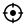
\includegraphics[width=0.5cm]{icons/map_turnpoint.pdf} &
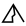
\includegraphics[width=0.8cm]{icons/map_mountain_top.pdf} &
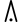
\includegraphics[width=0.7cm]{icons/map_obstacle.pdf} &

\includegraphics[width=0.7cm]{icons/map_pass.pdf} &
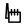
\includegraphics[width=0.8cm]{icons/map_power_plant.pdf} &

\includegraphics[width=0.7cm]{icons/map_tower.pdf} &
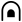
\includegraphics[width=0.6cm]{icons/map_tunnel.pdf} &
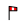
\includegraphics[width=0.6cm]{icons/map_weather_station.pdf} &
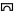
\includegraphics[width=0.8cm]{icons/map_bridge.pdf}
\end{tabular}
\caption{Points de virage non-posables}\label{fig:nonlandables}
\end{figure}

\section{Circuit en cours}

Le tracé du circuit en cours est représenté sur la carte par une ligne bleue pointillée.
Les secteurs et les aires des points de virage sont représentés par une surface surlignée en jaune.
Des cercles sont toujours représentés autour des points de départ et d'arrivée~;
des lignes y sont dessinées uniquement si ces points sont de type ligne.

Une ligne noire épaisse est affichée en permanence du planeur vers le prochain point de virage du circuit en cours.
Cette ligne peut pointer directement vers le point de virage, ou bien donner la trace d'un chemin contournant
relief et espaces aériens, comme décrit en détails dans le paragraphe~\ref{sec:route}.

\begin{center}
\begin{tabular}{c c c}
\emph{Départ/arrivée} & \emph{Secteur} & \emph{Cylindre} \\
\includegraphics[angle=0,width=0.3\linewidth,keepaspectratio='true']{figures/cut-startfinish.png} &
\includegraphics[angle=0,width=0.3\linewidth,keepaspectratio='true']{figures/cut-sector.png} &
\includegraphics[angle=0,width=0.3\linewidth,keepaspectratio='true']{figures/cut-barrel.png}
\end{tabular}
\end{center}


\section{Relief et topographie}\label{sec:terrain_topo}

Les éléments topographiques affichés sur la carte sont~:
\begin{itemize}
\item Routes principales, sous forme de lignes rouges
\item Fleuves et rivières, sous forme de lignes bleues
\item Grandes étendues d'eau (lacs), zones bleues
\item Grandes villes, zones jaunes
\item Villages et petites villes, petits diamants jaunes
\end{itemize}
Les villes et villages sont écrits en italique.

Le relief est coloré en fonction de l'altitude et optionnellement ombré suivant la direction du soleil ou la direction du vent. Les reliefs non valides ou sous le niveau de la mer sont représentés en bleu.

\menulabel{\bmenug{Affich. 2}\blink\bmenut{Relief}{On/Off}}
\menulabel{\vspace{1cm}\bmenug{Affich. 2}\blink\bmenut{Topo.}{On/Off}}

Le relief est ombré pour améliorer sa lisibilité.
Par défaut, l'éclairage virtuel utilisé est celui du cap du vent estimé.
Ainsi, les faces les plus claires sont les faces portantes, les faces sombres sont sous le vent.
L'ombrage en fonction de la position du soleil est aussi implémentée.
Si l'ombrage des pentes est configuré pour ``Soleil'', les pentes les plus claires suivent l'heure de la journée de façon très naturelle.
L'ombrage et la clarté globales sont paramétrables. \config{shading}

L'affichage du relief et de la topographie peuvent être activés/désactivés par les menus.

\begin{center}
\begin{tabular}{c c}
Topographie & Relief \\
\includegraphics[angle=0,width=0.4\linewidth,keepaspectratio='true']{figures/cut-topo.png} &
\includegraphics[angle=0,width=0.4\linewidth,keepaspectratio='true']{figures/cut-terrain.png}
\end{tabular}
\end{center}

Si la carte de relief n'est pas chargée (ou si son affichage est sur Off), le fond de la carte est blanc. Tout relief sous le niveau de la mer est représenté en bleu. Si vous volez en dehors de la carte ``relief'', le fond de carte sera aussi blanc.

\subsection*{Étiquettes sur la carte}\label{sec:maplabels}

L'écran peut contenir trop d'information et être peu lisible.
Il est alors possible de ne plus montrer les étiquettes des points de virage en modifiant le menu ``\emph{Étiquettes}''.
\menulabel{\bmenug{Affich. 2}\blink\bmenut{Étiquettes}{Aucun}} 

D'autres options pour diminuer l'encombrement de l'écran sont disponibles~:

\jindent{\bmenuth{Étiquettes}{Circuit \&}{Aérodromes}}{Affiche les noms des points de virage du
circuit en cours et de tous les aérodromes (basé sur les attributs des points de virages du
fichier de points de virage). Les autres points de virage sont représentés mais sans étiquette}
\jindent{\bmenut{Étiquettes}{Tous}}{Affiche les noms de tous les points de virage}
\jindent{\bmenuth{Étiquettes}{Circuit \&}{Terrains}}{Affiche les noms des points de virage du
circuit en cours et de tous les terrains posables (basé sur les attributs des points de virages du
fichier de points de virage). Les autres points de virage sont représentés mais sans étiquette}
\jindent{\bmenut{Étiquettes}{Circuit}}{Affiche uniquement les noms des points de virage du circuit en cours}

Dans tous les cas, le format des étiquettes reste paramétrable dans le menu de configuration ``\emph{Affichage de la carte / Points de virage}'. \config{labels}

\section{Trace sol}\label{sec:trail}

Une ``trace sol'' optionnelle est dessinée sur la carte et montre le trajet passé du planeur.
La couleur et l'épaisseur de la trace sont configurables en fonction de l'altitude ou de la valeur du variomètre.

\begin{center}
\includegraphics[angle=0,width=0.8\linewidth,keepaspectratio='true']{figures/snail.pdf}
\end{center}

Si un Vega ou un autre variomètre intelligent est connecté avec un sortie ``Netto'',
la valeur du vario Netto est utilisée. Alors la couleur et l'épaisseur de la trace sol
représentent la vitesse verticale de la masse d'air à la place de celle du planeur.

\config{snailtype}
La longueur de la trace sol peut être choisie entre \emph{Off}, \emph{courte} (environ 10~minutes),
\emph{longue} (environ une heure) ou encore \emph{complète} (depuis le début du vol).
Ce réglage peut être permanent en utilisant le menu de configuration \config{snailtrail} ou temporaire à l'aide du menu.
\menulabel{\bmenug{Affich. 2}\blink\bmenut{Trace}{Complet}} 

Quel que soit  le mode de trace choisi, en mode ``spirale'' la trace est courte afin de laisser la carte lisible.

Dans le but d'aider au centrage des ascendances quand il y a du vent, la trace sol en spirale
peut être compensée artificiellement en fonction du vent (dérive compensée en spirale).
De cette façon, la trace sol fait référence au vent et non plus au sol. Comme les thermiques
se déplacent aussi avec le vent, la trace sol compensée donne une meilleure
indication de la position du thermique par rapport au planeur.

La figure suivante en montre l'exemple. Quand la compensation de la dérive en spirale est activée
(figure de droite), le planeur semble tourner dans une colonne verticale plutôt que dans une colonne inclinée (figure de gauche).

\begin{center}
\includegraphics[angle=0,width=0.8\linewidth,keepaspectratio='true']{figures/traildrift.png}
\end{center}

\config{traildrift}
L'activation de la ``dérive compensée en spirale'' se fait dans le
menu de configuration du vent.  La compensation n'a lieu qu'en spirale~: la trace sol en transition n'en tient pas compte.
Le paramétrage peut se faire aussi avec fenêtre de configuration du vent.
\menulabel{\bmenug{Config. 1}\blink\bmenus{Vent}}

L'affichage de la dérive est aussi utile afin de montrer plus clairement
l'existence d'une inclinaison des thermiques due au cisaillement par le vent.

L'épaisseur de la trace sol peut être agrandie en fonction de la valeur du vario\config{trailscaled}.


\section{Marques}\label{sec:markers}

Les marques sont représentées par de petits drapeaux (a) sur la carte. Les marques peuvent être 
placées à la main en appuyant sur un bouton ou automatiquement. Un exemple d'utilisation
en mode automatique est de placer une marque à chaque entrée en mode ``spirale'', 
une façon simple de repérer tous les thermiques rencontrés.

\menulabel{\bmenug{Nav. 2}\blink\bmenug{Marquer}}
Les marques ne sont pas conservées sur la carte quand on éteint \xc.
Cependant, la position de toutes les marques est ajoutée au fichier \verb|xcsoar-marks.txt|.

\section{Marques de thermiques}

En montée dans les thermiques, des marques sont créées automatiquement et
affichées à l'écran. La position des 20~derniers thermiques est
stockée jusqu'à la fin du vol. 
\sketch{figures/thermalhistory.png}
Cette historique des thermiques est accessible par la
fonction ``Qu'y-a-t'il ici~?'', de la même façon que les autres marques et les points de virage.

En sélectionnant une marque sur la carte, vous obtenez la fenêtre suivante~:
\begin{center}
\includegraphics[angle=0,width=0.8\linewidth,keepaspectratio='true']{figures/marque_panel.png}
\end{center}

\section{Zone atteignable en plané}\label{sec:reach}

La limite de la zone atteignable en plané est représentée par
une ligne pointillée noire et blanche. Elle donne le contour de la zone
que peut atteindre le planeur avant d’arrivée à la hauteur minimale (hauteur d'arrivée).
La zone atteignable montre les trajectoires dans toutes les directions, avec possibilité de prendre en compte les trajectoires contournant
des reliefs. Cette fonctionnalité est utile pour estimer la rayon d'action
lorsque l'on est bas et que l'on recherche une ascendance, mais aussi lorsque l'on vole
en montagne.

Les calculs peuvent être configurés \config{turningreach} avec deux niveaux de détail~:
\begin{description}
\item[En ligne droite] Si le mode ``contournement'' est désactivé, alors la
zone atteignable montre la plus grande distance que le planeur peut parcourir en arrivée dans toutes les directions et en
ligne droite. La limite ressemble alors à une boucle fermée autour du planeur.

\begin{center}
\includegraphics[angle=0,width=0.8\linewidth,keepaspectratio='true']{figures/reach1.png}
% CUTOUT SHOWING GLIDE RANGE FOOTPRINT.  NO TOPOGRAPHY, FULLSCREEN, NO TASK. TURNING=FALSE
\end{center}
 
\item[Contourne] Si le mode ``contournement'' est activé, alors la zone atteignable montre la 
plus grande distance que le planeur peut parcourir en arrivée dans toutes les directions, 
même en contournant des obstacles\footnote{Le nombre maximum de contournements est
de trois, et aucun contournement ne peut faire plus de 90°.}.  La
limite ressemble alors à une boucle fermée autour du planeur, mais peut aussi 
inclure des trous indiquant des sommets de montagne que le planeur ne peut pas atteindre
sans reprendre d'altitude.

\begin{center}
\includegraphics[angle=0,width=0.8\linewidth,keepaspectratio='true']{figures/reach2.png}
% CUTOUT SHOWING GLIDE RANGE FOOTPRINT.  NO TOPOGRAPHY, FULLSCREEN, NO TASK. TURNING=TRUE
\end{center}

\end{description}

L'affichage peut être configuré afin de rendre floue la zone
non atteignable. \config{gliderange}
La trajectoire d'arrivée prend en compte la hauteur du planeur au-dessus du relief
en considérant la garde au sol (voir paragraphe~\ref{sec:safety-heights}).
Si cette marge n'est pas conservée, une croix rouge apparaît sur la carte à l'endroit de la violation.
Si un objectif est sélectionné, le calcul est effectué en ligne droite vers cet objectif.
Si aucun objectif n'est sélectionné, le calcul est effectué avec le cap actuel.

Si ``zone atteignable en plané'' est activée, alors la possibilité d'atteindre des points
de virages posables est utilisée par le mode ``Abandon de circuit'', par la liste des ``dégagements'',
et par l'affichage des points de virage posables sur la carte.

Il faut noter que les calculs du circuit en cours ne sont pas impactés par les calculs de zone atteignable en plané.
Par exemple, la flèche d'altitude nécessaire dans la flèche d'arrivée
ou les données du circuit affichées dans les InfoBoxes ne prennent pas en compte la ``zone atteignable en plané''.

Les calculs de ``zone atteignable en plané'' sont utilisés pour la trace au sol de la zone de local,
pour les hauteurs d'arrivée sur des points posables, par le mode ``Abandon de circuit'' et par la fenêtre des dégagements.
Les performances du planeur et le calage du MacCready utilisés pour ces calculs sont paramétrables\config{reachpolar}~:
\begin{description}
\item[Circuit] La valeur de calage du MC utilisée pour le circuit.
\item[MC de sécurité] Une valeur configurable, habituellement faible, de calage du MacCready doit être entrée par le pilote
afin de refléter des performances légèrement dégradées par rapport aux performances maximales du planeur. La marge de sécurité
dans la calcul de la zone atteignable est alors l'écart entre les performances maximales du planeur et les performances
du planeur en suivant la vitesse du vol avec la valeur du MacCready de sécurité.
\end{description}

\section{Fenêtres d'états (``\emph{Vol}'' et ``\emph{Temps}'')}\label{sec:flight-status}

Les fenêtres de dialogue des états sont réparties sur plusieurs onglets, donnant une information générale sur le
vol, le système, le circuit, les règles et les heures.
Ce sont des informations~; ils ne sont donc pas modifiables par l'utilisateur.
On y accède en faisant un ``S à angles droits'' sur l'écran ou par le menu.
\gesture{Gauche - Bas - Droite - Bas - Gauche}
\begin{quote}
\bmenug{Info. 2}\blink\bmenug{États}
\end{quote}

\subsection*{Vol}
L'onglet d'état du ``Vol'' affiche des informations à propos de la localisation du planeur. Il donne la position GPS, l'altitude, le
gain d'altitude maximal réalisé, le point de virage le plus proche, son cap et sa distance.
\sketch{figures/status-flight.png}

Cette fonctionnalité peut être intéressante pour communiquer votre position à d'autres.

\subsection*{Heures}\label{sec:time-status}
Cet onglet donne l'heure locale, la date et l'heure UTC,
la durée du vol, les heures de décollage et d'atterrissage, et
les heures de lever et de coucher du soleil.

Notez que les valeurs affichées dans les onglet d'``États'' sont statiques~:
les valeurs affichées sont celles valables à l'ouverture de l'onglet sélectionné.
\sketch{figures/status-times.png}
C'est-à-dire que la position, les durées, etc., ne sont pas mises à jour pendant que la page reste affichée.
Pour avoir les valeurs mises à jour, il faut ouvrir un autre onglet et de revenir l'onglet précédent. 


\section{Route}\label{sec:route}

Entre l'aéronef et l'objectif en cours, XCSoar peut calculer la route, en 3 dimensions,
en prenant en compte le relief et les espaces aériens. L'altitude de l'objectif est la hauteur
d'arrivée pour les points de virage d'arrivée. Elle peut être supérieure pour les points intermédiaires
selon le calcul du circuit, dans le but de le terminer. Le calcul de la route fonctionne en mode circuit normal, en mode ``Abandon'' et en mode ``Aller à''.

\begin{center}
\includegraphics[angle=0,width=1.0\linewidth,keepaspectratio='true']{figures/route3.png}
\end{center}

Le calcul d'optimisation de la route est basé sur la polaire du planeur.
Les routes sont optimisées pour minimiser le temps de vol. Par défaut, le calcul d'optimisation de route est inactif. Il peut être activé pour prendre en compte uniquement
le relief ou le relief et les espaces aériens. \config{routemode}

\begin{description} 
\item[Aucun] Calcul d'optimisation de route inactif.
\item[Relief] La route évitera le relief.
\item[Espace aérien]  La route évitera les espaces aériens.
\item[Les 2] La route évitera les espaces aériens et le relief.
\end{description}

Le relief est survolé en prenant en compte la hauteur minimum par rapport au relief (la garde au sol),\config{safetyterrain}
mais sans prendre en compte de distance minimale latérale.
Une route optimisée peut amener à une hauteur d'arrivée supérieure à la hauteur minimum d'arrivée~: par exemple si l'objectif se trouve juste derrière une montagne abrupte.

Les espaces aériens sont évités horizontalement par une marge d'environ 250~mètres. Il n'y a pas de marge verticale imposée. Des routes valides peuvent passer au-dessus ou au-dessous d'un espace aérien.

Si le calage MacCready est positif, les montées peuvent être permises en option
sur les routes calculées. La hauteur maximale de montée
peut être limitée à 500~m au-dessus du plafond du départ ou de l'objectif,
ou augmentée jusqu'au plafond défini comme plafond des thermiques.
\config{routeceiling} Les montées au-dessus de la plus haute altitude de départ ou de l'objectif sont pénalisées par un taux de montée plus faible que la
valeur réelle du MacCready.

Voici une partie des approximations et limitations du calcul de route~:
\begin{itemize}
\item quand les montées sont nécessaires (et autorisées) pour atteindre le prochain point de virage, les montées sont considérées comme ayant lieu en début de route.
\item les portions de transition en montée sont considérées comme étant à altitude constante, et équivalentes à une série de petites montées réparties le long de la route.
\item le long de la route, les virages de plus de 90° ne sont pas autorisés.
\item si l'algorithme de calcul de route n'aboutit pas, le calcul repasse en mode vol direct depuis la position actuelle du planeur vers l'objectif.
\end{itemize}


%%%%%%%%%%%%%%%%%%%%%%
\chapter{Provas de Cross Country}\label{cha:tasks}

O XCSoar fornece um sistema completo de gerenciamento de provas, no qual as provas podem ser editadas priorizando o vôo e quando se voa cross-country casual, podem ser modificadas durante o vôo.  Os waypoints podem ser avançados automaticamente ou manualmente.  Muitos cálculos do XCSoar são relativos aos pilões ou ao waypoint final.  A menos que uma prova real seja definida, o XCSoar irá criar uma função ‘casa’ com muitas das funções da prova, referindo-se à localização da decolagem.  Este capítulo também descreve o uso do registrador IGC com o XCSoar.

Existem três modos de provas disponíveis:

\begin{description}
\item[Prova ordenada] esta é a prova tradicional de cross-country, na qual consiste em um ponto de início, zero ou mais waypoints e um waypoint final.  Os pontos da prova têm que ser voados em ordem.
\item[Prova 'Ir Para'] voa-se para um único destino.
\item[Abortar prova] fornece opção para se voar ao próximo ponto pousável.
\end{description}

Observe que nos modos Ir para e Abortar Prova, a prova ordenada é retida e pode ser retomada posteriormente, preservando todas as estatísticas sobre as realizações na prova.

\subsection*{‘Ir para’ automático}

Se não houver nenhuma prova ordenada definida, haverá uma prova de ‘ir para’ definida automaticamente na decolagem, definindo a decolagem como ponto de destino ou o próximo aeródromo se estiver perto do ponto da decolagem.

Se houver ou não prova definida, o ponto de decolagem é sempre gerado e aparecerá na lista de waypoints para referências futuras.

Após a prova ordenada ter sido definida pela primeira vez, a função “ir para’ decolagem é ignorada.  Para retomar uma prova simples, use ‘Ir para’.


\section{Provas “Ir Para”}

As provas ‘Ir Para’ podem ser definidas selecionando um waypoint no mapa, pela lista de waypoints ou outro mecanismo, como por exemplo uma caixa de diálogo, e selecione  \bmenuw{Vá Para}. No modo de prova, selecione
\bmenug{Nav 2} e então \blink\bmenug{Prova} {Retomar} e a prova será retomada (se houver alguma).
 

\section{Editando provas}

Você pode editar provas de várias maneiras. Alguns métodos são mais úteis para editar antes do vôo e outros permitem que a prova seja modificada em vôo.  As provas podem ser salvas em arquivos e carregadas posteriormente e podem ser transferidas entre qualquer plataforma que rode o XCSoar.

\tip Também é possível salvar uma prova padrão e tê-la carregada automaticamente no início do XCSoar.  Uma utilização para isto é que você pode fazer uma prova com somente um waypoint e ajustá-lo para ‘casa’ – significa que o XCSoar será programado para voar de volta a esse ponto, que pode ser útil para se voar local.

As principais maneiras de configurar uma prova são:
\begin{itemize}
\item Usando a caixa de diálogo de edição de prova.
\item Selecionando o waypoint no mapa e adicionando-o à prova através da janela de diálogo de waypoint.
\item Carregando a prova a partir de um arquivo.
\end{itemize}

%Selecting the Task menu item will produce the Task dialogue box.  The
%list box on the left displays all of the turn points loaded into the
%system. Highlight the desired entries and using the "-$>$" and "$<$-"
%buttons assemble the desired task in the Task list box. As each turn
%point is added to the task a continuous display of the calculated task
%length is shown.  Tasks can be saved for recalling later using the
%"Save" button and recalled using the "Load" button.  Once the desired
%task is complete select "OK".
%
%{\it DIAGRAM SHOWING TASK DIALOG EDITING, WITH LABELED ARROWS POINTING
%TO THE USER INTERFACE ELEMENTS?}

Carregar uma prova através de um arquivo talvez seja útil em competição ou cross-country quando voado em grupo, já que um só piloto pode distribuir o arquivo aos outros, economizando tempo de todos para editar a prova.  Se não houver prova ativa no início, o XCSoar criará automaticamente uma prova contendo o waypoint ‘casa’.

O XCSoar salva a prova atual quando é desligado e carrega-a assim que ligado, permitindo que se possa desligar o XCSoar até voar novamente.

Os pontos da prova são preservados mesmo que o waypoint seja alterado.  Isto significa que, se você tem uma prova e altera um arquivo de waypoint e carregar a prova novamente, novos waypoints serão gerados para os pontos que estão faltando no novo arquivo de waypoint.



\section{Informação do Waypoint }
%Several ways of selecting a waypoint are available:
%\begin{itemize}
%\item Touch its name or the waypoint symbol on the map screen if it is visible.
%\item If the waypoint is in the active task, highlight the waypoint {\InfoBox}, 
%  then use the up/down arrow keys to select the desired waypoint, and press the
%enter key.
%\item From the Task dialogue, find and highlight the waypoint in
% the waypoint list, then press the 'Details' button.
%\end{itemize}
%The display will now show the waypoint details dialogue.

A janela de diálogo do waypoint descreve os detalhes deste ponto e tem suas funções de navegação como Ir, Inserir, Anexar à prova ou ajustar este waypoint à nova posição ‘casa’.  Pode ser acessado das seguintes formas:

\gesturespec{rd}ou menu \bmenug{Nav 1/2}\blink\bmenug{Prova},
\todonum{descr. tabular "Pilões"}
selecione um waypoint, clique novamente no waypoint para mostrar a janela de diálogo deste ponto, e então clique em\bmenuw{Detalhes}.

\gesturespec{dl}ou menu \bmenug{Nav 1/2}\blink\bmenug{Alternativos}
para mostrar os detalhes dos pontos pousáveis perto da aeronave.

\gesturespec{dr}ou menu \bmenug{Nav 1/2}\blink\bmenug{Lista Waypoint}
, selecione e\bmenuw{Selec} para selecionar o waypoint e mostrar os detalhes.

\gesturespec{urdl}or menu \bmenug{Display 1/2}\blink\bmenug{Pan On} para colocar o mapa em modo panorâmico, arrastando até o ponto desejado do waypoint, tocando seu nome ou seu símbolo

\bmenug{Info 1/3}\blink\bmenug{Oque aqui?}
para mostrar a lista de itens abaixo da mira da tela, ou seu dedo no mapa.


Os detalhes do waypoint contém duas páginas principais (acessadas através dos botões 
\bmenuw{$>$} e \bmenuw{$<$}). do waypoint, podem ser mostrados em páginas extras.

\subsection*{Detalhes do Waypoint}
\label{sec:waypointdetails}
Esta página contém texto descritivo da localização do waypoint, frequência de rádio e informações da pista (se houver esta informação no arquivo de waypoints), elevação, hora do nascer e pôr do sol, direção, distancia ao waypoint e altitude necessária para atingir o waypoint. Também há um botão 
\bmenuw{IR} para iniciar imediatamente a navegação a este waypoint.  Este botão cancela a prova atual.

\begin{center}
\includegraphics[angle=0,width=0.8\linewidth,keepaspectratio='true']{figures/dialog-waypointdetails0.png}
\end{center}

Como citado acima, a janela de diálogo do waypoint também mostra três formas de diferença de altitude (altitude adicional necessária para alcançar o waypoint a uma altura segura) para o waypoint correspondente:
\begin{description}
\item[Alt diff MC 0] Diferença de altitude com MC ajustado em 0.
\item[Alt diff MC safety] Diferença de altitude no ajuste de segurança/aborto de MacCready (veja seção  \ref{sec:safety-factor})
\item[Alt diff MC current] Diferença de altitude com o ajuste atual de MacCready.
\end{description}

Através da janela principal de waypoint, você pode acessar a segunda página usando os botões 
\bmenuw{$>$} e \bmenuw{$<$} no canto inferior esquerdo da tela.  
\subsection*{Menu de ações da prova}  
Esta página contém uma coluna de botões que permite várias ações:
\begin{description}
\item[\bmenuw{Substituir na prova}] substitui o waypoint ativo na prova pelo waypoint selecionado.
\item[\bmenuw{Inserir na prova}] insere o waypoint selecionado antes do waypoint ativo na prova.
\item[\bmenuw{Anexar à prova}] adiciona o waypoint selecionado ao final da prova.
\item[\bmenuw{Remover da prova}] remove o waypoint selecionado da prova.  Esta opção só estará visíviel se o waypoint selecionado está incluso na prova.
\item[\bmenuw{Selec como nova Casa}] ajusta o waypoint como ‘casa’.
\item[\bmenuw{Deslocar para waypoint}] alterna para o modo panorâmico e arrasta para o waypoint.
\end{description}

É uma boa idéia ajustar seu waypoint ‘casa’ na janela de diálogo de waypoints.  Isto faz o XCSoar iniciar sempre neste ponto, mesmo quando o XCSoar ainda não obteve sua posição de GPS.  Se não for fixada nenhuma posição 'casa', o XCSoar irá centrar no meio do mapa.

\subsection*{Informação do Aeródromo}
Esta página pode conter texto relevante sobre o aeródromo, incluindo pistas, frequências de rádio, padrões de tráfego e contatos.
\begin{center}
\includegraphics[angle=0,width=0.8\linewidth,keepaspectratio='true']{figures/dialog-waypointdetails1.png}
\end{center}

\subsection*{Imagem dos detalhes do Waypoint}
Esta página mostra uma imagem de satélite do waypoint.

\begin{center}
\includegraphics[angle=0,width=0.8\linewidth,keepaspectratio='true']{figures/dialog-waypointdetails2.pdf}
\end{center}
Como ajustar as informações de detalhes do waypoint estão na seção \ref{sec:airfield-details}

\section{A janela de seleção de Waypoint}\label{sec:waypoint-selector-dialog}

A janela de seleção do waypoint permite que se selecione facilmente de um grande banco de dados.  \gesturespec{dr}

Acionando a seleção ativa uma tela com um conjunto de filtros do lado 
\menulabelr{\bmenug{Nav 1/2}\blink\bmenug{Lista Waypoint}}
esquerdo da tela e uma lista de waypoints do lado direito da tela, coincidindo todas as condições dos filtros.  Há vários filtros disponíveis, que podem ser usados em conjunto, individuais ou sem filtro.
\begin{description}
\item[Nome] seleciona os waypoints começando com o caractere digitado.
\item[Distância] filtra os waypoints mais próximos do que a distância digitada.
\item[Direção] filtra os waypoints que não estão especificados na direção da aeronave.  A direção especial “HDG(0°)” filtra waypoints com até 30° de deslocamento para ambos os lados do sentido da aeronave.  Isto permite que o piloto aponte a aeronave a um grupo de waypoints e rapidamente possa achá-los.
\item[Tipo] filtra waypoints que não são do tipo especificado (pousáveis, aeroportos ou pilões) ou que aparecem em arquivos específicos.
\end{description}
Quando filtrados por nome e tipo, a listra é mostrada em ordem alfabética.  Quando filtrado por distância ou direção, a lista é ordenada por distância.  

\begin{center}
\includegraphics[angle=0,width=0.8\linewidth,keepaspectratio='true']{figures/dialog-waypointselect.png}
\end{center}

A lista pode ser rolada se houver mais de uma tela cheia de waypoints.  Para rolar a lista, simplesmente arraste com o dedo ou mova para baixo (ou para cima) a lista com o cursor. 

Selecionar um item irá resultar em um comportamento diferente, dependendo de qual função abriu o seletor de waypoints.  No uso normal, mostrará os detalhes do waypoint.

\section{Gerenciador de Tarefas}\label{sec:task-manager-dialog}
\begin{it}  O gerenciador de tarefas foi redesenhado se comparado com as versões anteriores do XCSoar.\end{it}
\gesturespec{rd}

O gerenciador de tarefas é usado para editar, visualizar, carregar, salvar em arquivo e declarar as provas de cross-country.
\menulabelr{\bmenug{Nav 1/2}\blink\bmenug{Prova}}

A primeira página é uma calculadora.  Mostra vários cálculos relativos à prova ativa, como descrito em detalhes abaixo:  Há botões para acionar os diálogos \bmenuw{Pilões}, \bmenuw{Gerenciar}, 
e \bmenuw{Regras}, bem como o botão \bmenuw{Fechar}.

\subsection*{Janela de Calculadora de Prova}\label{sec:task-calc-dial}
A janela calculadora de prova permite que o piloto veja o efeito de suas várias mudanças da prova no desempenho final.
\menulabelr{\bmenuw{Calculadora}}

Em vôo, a Calculadora de Prova também pode ser acessada da página de Análise.  Com as páginas Prova, Subida e Velocidade da Prova, aparece um botão chamado  \bmenuw{Calculadora} que vai diretamente à esta janela.
 



\begin{center}
\includegraphics[angle=0,width=0.8\linewidth,keepaspectratio='true']{figures/dialog-taskcalculator.png}
\end{center}

\begin{description}
%\item[Tempo da prova]  Este campo mostra o tempo da prova.
\item[Tempo Prova est]  este campo mostra o tempo total para completar a prova usando o ajuste de MacCready introduzido.
\item[Task distance]  This field displays the task distance remaining.
\item[Ajuste MacCready]  permite ao usuário ajustar o MacCready e ver seus efeitos no tempo de prova estimado.
\item[AAT range]  permite ao usuário ajustar os alvos dentro das áreas AAT, para ver o efeito no tempo estimado e distância da prova.
\item[Velocidade restante]  este campo mostra a velocidade estimada restante para a prova com o ajuste MacCready fornecido.
\item[MacCready Atingido]  este campo mostra o valor de MacCready atingido.
\item[Veloc Atingida] mostra a velocidade atingida.
 % at the achieved MacCready setting???
\item[Eficiência planeio]  100\% indica um desempenho perfeito de MacCready, maior que 100\% indica que o desempenho de MacCready é superado voando em estradas de nuvens.  Menor que 100\% é apropriado se você voa consideravelmente fora da rota.  Este valor estima sua eficiência de cruzeiro de acordo com o histórico atual de vôo com o valor de MacCready.    Os cálculos iniciam após a prova iniciada.
\end{description}
Veja seção ~\ref{sec:task-speed-estim} para mais detalhes da velocidade da prova e cálculos de MacCready realizados.

Fechando a janela, o valor digitado de MacCready será usado como ajuste. Se o botão \bmenuw{Fechar} for pressionado, o ajuste de MacCready não será afetado.

O botão \bmenuw{Pilões} para provas AAT , ajusta o alcance (aumenta ou diminui) para que o tempo estimado exceda o tempo designado para prova subtraído de 5 minutos. O alcance é ajustado amplamente, geralmente todos os alvos são configurados para ''auto", significando que o piloto não tem que ajustar manualmente o alcance para achar o caminho para a chegada no tempo designado, diminuindo o trabalho do piloto.
  
\subsection*{Pilões}
Esta opção mostra uma lista ordenada de pontos da prova atual.
\menulabelr{\bmenuw{Pilões}} 
Se não houver waypoints na prova atual, só haverá a opção \bmenuw{Adicionar Pilão}.  Clicando no waypoint da lista e depois em \bmenug{Selec} o mesmo será incluso na lista.  

\subsection*{Gerenciar}
Esta página permite acionar todas as operações necessárias para criar novas provas ou gerenciar
\menulabelr{\bmenuw{Gerenciar}}as existentes.


\begin{itemize}
\item [\bmenuw{Nova Prova}] Apaga a prova atual e limpa as regras da prova, deixando os valores padrões.
\item [\bmenuw{Declarar}] Se houver um registrador externo conectado, permitirá que se envie a prova atual para o logger e faça a declaração.
\item [\bmenuw{Procurar}] Mostra uma lista de provas salvas, permitindo o piloto carregar uma prova já realizada.  Observe que esta opção irá sobrescrever a prova atual.
\item [\bmenuw{Salvar}] Salva a prova atual.  Clicando em 
  \bmenuw{Salvar} o piloto será questionado a entrar com um nome de arquivo para ser salvo.
\end{itemize}

\subsection*{Regras}
Os valores neste menu dependem do tipo de prova selecionado.  Clicando 
\menulabelr{\bmenuw{Regras}} em qualquer valor existente abrirá outro menu permitindo ao piloto selecionar um valor diferente para esta regra.  Os tipos de provas serão apresentados mais a frente.

Também clicando em \bmenuw{Regras} novamente, permite alternar entre uma visão geral da prova e retornar para a tela anterior.  

\section{Tipos de provas}
O XCSoar define três tipos diferentes de prova: Racing, AAT, e Insígnias/recordes FAI.

A descrição detalhada dos tipos de prova está listada adiante, mas este manual não pretende reformular as regras da FAI ou contestar os tipos de provas.  O leitor é forçado a se tornar familiar com cada tipo de prova, consultando as regras da FAI em \url{http://www.fai.org}. 


\subsection*{Competindo}
(Também conhecida como “prova atribuída”).  A prova atribuída envolve voar sobre alguns pilões em uma ordem específica.  Selecionando o tipo de prova permite ao piloto entrar com os seguintes parâmetros: 
  \begin{description}
  \item [Arm start manually] se ajustado para “Ligado”, alguns botões extras serão mostrados em ordem para \bmenug{Armar largada} bem como \bmenug{Desarmar largada} no menu \bmenug{Nav 1/2}, controlando a condição de detecção do Start.
  \item [Start open time] É a hora quando o Start deve abrir. 
  \item [Start close time] Hora em que a área de Start deverá fechar.
  \item [Veloc máx largada] esta é a velocidade máxima permitida na área de start.  Deve ter valor 0 se não houver limite.
  \item [Altura máx largada] maior altitude acima da altura de referência do start (AGL ou MSL), cuja prova pode ser iniciada.  Se não houver limites, o valor deverá ser 0.
  \item [Ref altura largada] especifica a altura máxima acima da altura de referência ao nível do solo do ponto de start (AGL ou MSL).
  \item [Altura mín chegada] Taltura mínima baseada na altura final de referência (AGL ou MSL) que a prova pode ser finalizada.  Deve ser ajustada em zero se não houver limite. 
  \item [Altura final de ref.] altura mínima referenciada ao nível do solo para o ponto final da prova (AGL ou MSL).
% \item [FAI start/finish rules] If enabled, this task type has no max. start height 
%   or max. start speed.  Finish height reference is set to AGL and finish height 
%   is 1000m below the start height \todonum[inline]{Is this description correct?}
  \end{description}
  
\subsection*{Área de prova atribuída (AAT) e Prova com área modificada (MAT)}
(Também conhecida como “prova de pilão” ou TAT).  Este tipo de prova é através de áreas designadas (restringidas às áreas com cilindros ou setores).  Há um tempo mínimo aplicado.  As opções de regras para esta prova incluem:
  \begin{description}
  \item [AAT min. time]  este é o tempo mínimo para realizar a prova. Consulte um especialista para as penalidades se finalizar em tempo abaixo do mínimo.  O tempo nesta opção é dado em minutos.
  \item [Outras regras] todas as outras regras permanecem as mesmas para este tipo de competição.
  \end{description}


\subsection*{Insígnias FAI / recordes}
  \begin{description}
  \item [Regras de início/ final FAI] se ajustado para “Ligado”, somente a hora de início pode ser definida.  Se a opção for “Desligado”, todas as outras regras da prova podem ser alteradas dos padrões da FAI.
  \end{description}

Uma vez definido o tipo de prova e as regras de início e fim também foram definidas conforme descrito acima, é necessário definir as propriedades de cada waypoint da prova.

\section{Regras da prova para os pilões}\label{sec:task-rules}

A janela de \bmenuw{Pilões} mostra uma lista de waypoint da prova. 
\menulabelr{\bmenuw{Pilões}} Se não houver pilões definidos, a tela irá mostrar uma lista vazia.  Com \bmenuw{Adicionar Pilão}, botões acima e abaixo, e \bmenug{Fazer Final} a lista é criada.  Os waypoints podem ser o ponto de início, pilão ou ponto final.  Selecione qualquer waypoint na lista ou clicando em \bmenug{Editar Ponto} mostrará as definições deste waypoint.  Clicando em \bmenuw{Mudar Tipo} mostrará uma série de opções de tipos de pilões disponíveis.  As definições de cada tipo são mostradas na parte inferior da tela.

Uma série de regras de prova podem ser usadas quando se monta uma prova, incluindo o triangulo FAI e Prova de Área Atribuída (AAT).  Muitas características da prova também podem ser personalizadas.

As linhas de início e fim são centralizadas nos seus waypoint e alinhadas perpendicularmente aos waypoints anteriores e posteriores, respectivamente.

Os pilões de setor são segmentos alinhados a 90° com a bissecção dos waypoints anteriores e posteriores, comumente usados em provas FAI.  Também há opções para os triângulos ingleses BGA e alemães DAeC.  

\subsection*{Tipos de start point}
As condições para se fazer o start dependem do tipo de início:
\begin{description}
\item[Start Cylinder] Quando a aeronave deixa a área do cilindro.
\item[Start Line] Quando a aeronave cruza a linha de início.
\end{description}

\subsection*{Tipos de pilões}
As condições para se fazer um pilão válido dependente de seu tipo:
\begin{description}
\item[Setor FAI] quando a aeronave entra na zona de observação (ZO), definida por um segmento e distância radial do waypoint.  O segmento é definido por um arco de 90° centrado sobre a bissetriz das pernas de entrada e saída, com distância de 20km.  
\item[Keyhole Sector (DAeC 0.5/10 sector)] é quando a aeronave entra em uma zona de observação, definida por um segmento e distância do waypoint. O segmento é definido por um arco de 90° centrado na bissetriz das pernas de entrada e saída, com distância de 10km.  A zona de observação também inclui um cilindro de 500m.
\item[Turnpoint Cylinder]  quando a aeronave entra em uma zona de observação definida por uma distância radial do waypoint.
\item[BGA Enhanced Option Fixed Course Sector]  quando a aeronave entra na zona de observação definida por um segmento e uma distância radial do waypoint.  O segmento é definido por um arco de 180° centrado na bissetriz das pernas de entrada e saída, com distância de 10km.  A zona de observação também inclui um cilindro de 500m (regras britânicas).
\item[Area Cylinder (AAT)]  e
\item[Area Sector (AAT)]  quando a aeronave entra na zona de observação definida por uma distância radial do waypoint e segmento para áreas de setores.

\end{description}

\subsection*{Tipos de Pontos Finais}
A realização da prova depende do tipo de ponto final.
\begin{description}
\item[Finish Cylinder] Quando a aeronave entra na área do cilindro.
\item[Finish Line] Quando a aeronave cruza a linha de chegada.
\end{description}

O avanço automático é disparado sempre que uma condição é alcançada.  Para iniciar uma prova AAT, mista ou Corrida, a prova tem que ser armada antes.

\tip As regras da competição podem ser definidas em um arquivo para serem distribuídas ao grupo de pilotos e comissão técnica, para que todos os competidores tenham as mesmas regras!

As regras adicionais da prova para inícios e finais válidos também devem ser especificadas.  O Start deve ter uma altitude máxima acima do solo e velocidade máxima definidas.  Os finais devem ter uma definição da altitude mínima acima do solo.  Estes parâmetros são definidos na página “Padrão das Provas”, nos ajustes das configurações.

Para provas não AAT, há opção disponível para ajustar a altura mínima final de acordo com a regra FAI, pela qual estabelece a altura mínima de chegada deve ser 1.000 metros acima da altura de largada.


%Need to add a section describing how to start the task%


\section{Avançando e reiniciando provas}\label{sec:advanc-rest-tasks}
Um waypoint, a qualquer tempo, pode ser atribuído como waypoint ativo na prova.  O waypoint ativo é usado para cálculos e mostrar informações de navegação, isto é, o piloto é direcionado a voar para este waypoint ativo (também conhecido como próximo waypoint na descrição do Infobox no Capítulo ~\ref{cha:infobox}).

Durante o vôo, a indicação de direção para o próximo waypoint é contínua.

A altitude necessária para completar a prova é calculada pela rota atual, iniciando com a posição atual da aeronave, passando pelos pilões até o ponto final.

A mudança do waypoint é feita automaticamente ou talvez manualmente.  O start da prova e pontos AAT são casos especiais que necessitam que se “arme” os pontos da prova antes que o sistema avançe para o próximo ponto da prova, uma vez que este ponto foi atingido.  Todos os pontos da prova serão avançados automaticamente ao próximo ponto assim que o último ponto for atingido.

Para provas não-Corrida, não é necessária nenhuma interação do usuário para avançar pela prova – o sistema irá automaticamente avançar a cada ponto da prova assim que o ponto for alcançado.  O piloto deve avançar ou retroceder manualmente o ponto ativo selecionando os menus, respectivamente:
 \bmenug{Nav}\blink\bmenug{Pto virada anterior} and
\bmenug{Nav}\blink\bmenug{Próx. Pto Virada}.

Os botões \bmenug{Pto virada anterior} e
\bmenug{Próx. Pto. Virada} mostram rótulos dinâmicos que indicam a ação a ser feita se selecionados.

Para os pontos de provas que necessitam serem armados, \bmenug{Próx. Pto. Virada} se torna 
\bmenug{Armar ponto} se o ponto não for armado;  se estiver armado, então aparecerá
\bmenug{Próx. Pto. Virada} permitindo o avanço manual.  O
\bmenug{Pto. virada anterior} aparecerá como\bmenug{Desarmar ponto}se o ponto estiver armado e vice versa.  Igualmente para provas de corrida, estes itens de menu se atualizam para armar os pontos de início.  Se o próximo ponto de virada é o ponto final, o rótulo se altera para tal.

As mensagens de estado são fornecidas para os pontos da prova que necessitam serem armados, como um lembrete para armar o ponto de virada quando o piloto está pronto para avançar ao próximo waypoint.  Para iniciar, é dado um alerta que a aeronave está no cilindro de start ou atrás da linha, como um lembrete de “armar” se necessário.  

Para PC e Pocket PC com tela de toque, o usuário pode manualmente navegar através dos waypoint selecionando a infobox do waypoint e apertando as setas para cima e para baixo.

Veja a seção ~\ref{sec:task-rules} para detalhes das regras de observação.

Se um usuário navegou até o waypoint manualmente, não significa que a aeronave passou efetivamente pelo waypoint!  Todavia, esta facilidade é útil para forçar um reinicio da prova ou para pular um waypoint quando se voa cross-country casual.

\tip As provas podem ser reiniciadas manualmente navegando através dos waypoint do início.

Em todos os modos, se a aeronave reentrar na zona de start ou cruzar o início do start anterior, a prova será automaticamente reiniciada.

Quando se seleciona  \bmenug{Pto. virada anterior}, o gatilho que detecta o auto avanço para aquele waypoint é apagado, significando que o gerenciador de prova aguarda a aeronave voar para aquela zona de observação (ZO) novamente antes de continuar a prova o piloto deve selecionar \bmenug{Próx. Pto. Virada} para avançar para o próximo waypoint da prova.

Um bip do sistema e uma mensagem é mostrada no avanço da prova/waypoint.  A mensagem é mostrada quando o sistema avança até o waypoint da prova automaticamente ou manualmente em modo “armado”, quando está armado e a aeronave está no setor:
\begin{description}
\item[Início da Prova]  aparece quando a aeronave cruzou o start ou saiu do setor de início.  Pode ser repetido a qualquer hora.
\item[Próx. Pto. Virada]  aparece quando a aeronave entrou no setor de observação para fazer o pilão.  Assim que o botão 
 \button{Armar virada} Para o modo de rearme manual, se a aeronave entrou no setor de observação, ao apertão este botão irá fazer o gerenciador de provas entender que a virada foi postergada para outro momento.
\item[Final da Prova]  aparece quando a aeronave cruzou a linha de chegada ou entrou no cilindro de final.  Ambos ocorrem no modo avançado. 
\end{description}


\section{Starts alternativos}\label{sec:alternate-starts}

%Alternate start points are skipped for XCsoar 6.0, but
%will potentially brought back in a next release. 

%\todonum[inline]{Alternate start points are skipped for XCsoar 6.0, but
%will potentially brought back in a next release. This section can thus be
%treated as obsolete. }

O sistema de provas permite que se defina start alternativos:

\blink\bmenuw{Pilões} selecione o início, \menulabelr{\bmenug{Nav 1/2}\blink
\bmenug{Prova}}\bmenuw{Editar Ponto}\blink\bmenuw{Habilitar Starts Alternados}

Na página de ponto de start do Gerenciador de Tarefas, mude para \bmenuw{Habilitar Starts Alternados}. Outra tela aparecerá para definir o ponto alternativo.  Neste caso, os pontos de start devem ter sidos definidos previamente.  Depois de selecionado \bmenuw{Habilitar Starts Alternados} e teclado \bmenuw{Edit Alternates}. Depois de selecionado\bmenuw{Add Alternates Starts} e pressionando 
\bmenuw{Realocar} abrirá a janela para seleção de waypoints.
 
Tendo configurado alguns starts alternativos, o método “próximo waypoint” será novamente aumentado.  Antes da detecção de um start válido e tendo armado o start manualmente, no menu de botões irá aparecer  \bmenug{Próximo Start}.

Resumindo, todos os rótulos dinâmicos em \bmenug{Nav 1/2} mostrarão os comandos a serem executados para selecionar os waypoints e condições, tanto na ordem normal como inversa.

%\begin{center}
%\includegraphics[angle=0,width=0.8\linewidth,keepaspectratio='true']{figures/%dialog-startpoint2.png}
%\end{center}
  
%  To edit the start points, move the cursor to an item in the list on
%  the right side of the dialogue, and press enter.  This opens the
%  waypoint selector dialogue, to allow selection of the waypoint.  This
%  process can be repeated several times for several alternate start
%  waypoints.  Press the `clear' button to clear all alternate start
%  points.

%  Each start sector is fixed to the same type (line/cylinder) and size
%  (start radius) defined in the task waypoint page.

%  Note that the task start point should be included in the alternate
%  start location list. 

%\begin{center}
%\includegraphics[angle=0,width=0.8\linewidth,keepaspectratio='true']{figures/%dialog-startpoint3.png}
%\end{center}

%\begin{center}
%\includegraphics[angle=0,width=0.8\linewidth,keepaspectratio='true']{figures/%dialog-startpoint4.png}
%\end{center}

%  In flight, any time you cross a start line (or exit a start
%  cylinder), this will start the task at that particular alternate
%  start.  Task statistics are recalculated for the start sector you
%  last flew through.  All alternate start sectors are shown on the
%  map.  You can re-start simply by flying through the start sector
%  again or another start sector.  This automatic re-start will only
%  happen if the active waypoint is the first turnpoint after the
%  start, or the start itself.

%  When the waypoint advance mode is `Arm' or `Arm Start', then a start
%  is only recognised by XCSoar if the advance trigger is armed.

%  If desired, alternate start points may be selected as the active
%  waypoint by selecting the previous waypoint.  Continuing to select
%  the previous waypoint will cycle through all alternate start points.

\section{Abortar/retomar a prova a Alternativos}

Se as condições atmosféricas ficarem piores, você poderá concluir que será impossível completar a prova.  Neste caso, você poderá instruir o XCSoar para “abortar” a prova e lhe orientar a procurar um pouso seguro.  Uma prova ordenada pode ser abortada de diversas maneiras, tanto pela seleção do waypoint e executar o comando ‘ir para’ ou acionando o modo de aborto.  Em ambos os casos, a prova atual poderá ser retomada.

\subsection*{Abortando a prova}\label{sec:taskabort}
Acionando o modo de aborto, força o XCSoar a entrar em modo especial de planeio final.  Para se aprofundar em modos de vôo, veja a seção \menulabelr{\bmenug{Nav 2/2}\blink\bmenug{Prova Abortar}}.  Para se aprofundar em modos de vôo, veja a seção  \ref{sec:flightmodes}. Neste modo de vôo, a opção de configuração “alcance polar” determina qual a altura de chegada do waypoint, usando o valor de segurança de MacCready para abortar a prova.  O padrão é usar o MacCready de segurança.  Quando se alterna para o modo de aborto, o valor de MacCready é alterado para seguro, mesmo que seja mais baixo que o valor atual em vôo.

Com o modo de aborto, a prova é desabilitada.  No mapa haverá pontos para os próximos pontos pousáveis para ajudar na decisão do piloto.  Enquanto durar o vôo, o grupo de pontos pousáveis é mantido permanentemente.  Os pontos pousáveis podem se alterar dinamicamente quando estiver em modo de aborto portanto, a qualquer momento vários pontos pousáveis são mostrados e qualquer um deles pode ser selecionado como waypoint ativo.  Mesmo que não haja ponto pousável dentro do planeio, os raios serão desenhados na tela
\sketch{figures/abort-low.png} 
Se as condições melhorarem, a prova pode ser retomada selecionando o mesmo botão de menu, agora indicando \bmenug{Prova Retomar}. O ponto ativo é então restaurado bem como todos os outros detalhes da prova.

\subsection*{Alternativos} \label{sec:alternates}
Os pontos alternativos são mantidos durante o vôo, refletindo que o piloto mantém seus olhos nestes pontos.\menulabelr{\bmenug{Nav 1/2}\blink
\bmenug{Alternativos}}.  Seis opções de pousos serão mantidas.  São filtradas pelos critérios de configuração (simples, prova ou casa). \config{alternatesmode} 
Escolhendo Prova ou Casa, há a inserção de alguns conceitos na apresentação dos alternativos, enquanto você está sendo orientado pela prova. 

Igualmente quando se tem toda a lista de waypoints, as informações adicionais podem ser vistas clicando em \bmenuw{Detalhes} antes de decidir para qual ponto se navegara.  Selecione um waypoint da lista e clique em \bmenuw{Ir Para}.
\sketch{figures/alternates_list.png}

Todavia, os itens na lista de alternativos obedecem regras diferentes e interagem da mesma forma com a prova atual.  Escolher um ponto na lista de alternativos aborta a prova; uma vez que as condições melhores, o resumo da prova pode ser realizado pelo botão já mencionado.


\section{Estado da prova }\label{sec:task-status}

A janela de diálogo de estado fornece um resumo das informações importantes da prova.   
\gesturespec{ldrdl} Pode ser útil para dar uma visão geral da prova enquanto se usa as Infoboxes por outros motivos.  A janela de estado pode ser consultada para se confirmar se um start válido foi detectad, bem como o progresso na prova
\menulabelr{\bmenug{Info 2}\blink\bmenug{Estado}}
.  Esta janela também pode ser acionada por menu ou gesto, descrevendo um “S”.   Pode-se ver as abas “Prova” e “Regras”.

A aba de prova mostra o tempo AAT, distâncias alcançadas, tempos restantes e da prova.  Aba das regras mostra a validação do start/final de acordo com as regras da prova.

\begin{center}
\begin{tabular}{c c}
Prova & Regras \\
\includegraphics[angle=0,width=0.4\linewidth,keepaspectratio='true']{figures/status-task.png} &
\includegraphics[angle=0,width=0.4\linewidth,keepaspectratio='true']{figures/status-rules.png} \\
\end{tabular}
\end{center}

\section{Provas de Áreas Atribuídas}\label{sec:aat-tasks}

\subsection*{Alvos AAT}

Um alvo é um ponto dentro de uma área AAT em que o piloto deve se dirigir.  Estes alvos podem ser movidos dentro da área AAT, portanto o piloto pode configurar a distância efetiva da prova.  Os alvos devem ser configurados no chão, durante o planejamento da prova e modificados durante o vôo.

Quando se voa uma prova AAT, o sistema de navegação direciona a aeronave para o alvo e as estatísticas como distância ao waypoint também são relativas ao alvo, ao invés do waypoint da área AAT.

O avanço automático do waypoint da prova não é acionado quando se entrar numa área AAT única.  O piloto tem que armar a virada manualmente para avançar para o próximo pilão.  Quando se arma um pilão AAT durante o vôo através da zona de observação, há o acionamento do modo de otimização da prova para capturar a realização dos alvos AAT e a atualização de toda a prova.   Veja a seção ~\ref{sec:advanc-rest-tasks} 
para mais detalhes.

\subsection*{Movendo manualmente os alvos}

Para fazer a especificação dos alvos diretamente, a localização destes é definida por alguns parâmetros que determinam quão longe da distância mínima ou máxima o alvo está. É expresso em porcentagem.  Por exemplo, um alcance ajustado em 100\%, o alvo é posicionado para fornecer a distância máxima possível de onde está o alvo.  Com o alcance ajustado em -100\%, o alvo é posicionado para fornecer a mínima distância total da prova.

O alcance zero determina a distância nominal da prova:  para setores, a prova é a metade da bissetriz radial; para cilindros, o alvo é o centro do cilindro.

A janela de cálculo de prova (veja seção ~\ref{sec:task-calc-dial}), mostra o percentual médio sobre todos os pilões do campo de alcance AAT.  Os alvos podem ser modificados individualmente através da janela de diálogo de cálculo de prova.


\subsection*{Alvos AAT e Calculadora de Prova}

O uso mais comum dos alvos quando se voa AAT são:
\begin{itemize}
\item Ajustar o MacCready esperado, lastro e ajustes de vento para o vôo, usando as janelas de configurações de vôo e ajustes de vento.
\item Definir a prova como normal através do editor de provas.
\item Baseado no julgamento do piloto de como está a condição e como algumas áreas são mais difíceis que outras, os alvos podem ser ajustados individualmente para cada pilão.  O campo ETE na visão do alvo comparado com o tempo mínimo assumido é mostrado como um Delta T para verificar se a prova planejada é eficiente e longa o suficiente.
\item Durante o vôo, se as situações mudarem como o ajuste de MacCready ou vento, a calculadora de prova pode ser mostrada para estimar o tempo de prova, novamente comparando com o tempo mínimo configurado para a prova.
\item Se o piloto decide estender ou reduzir o vôo, todos os pontos restantes podem ser modificados através da calculadora de prova.
\end{itemize}

A calculadora de prova também permite ao piloto perguntar (e ajudar na resposta) “O que acontece”, por exemplo: 
\begin{itemize}
\item O que acontece se as condições melhorarem? O ajuste de MacCready pode ser aumentado e o piloto pode ver se há ajustes suficientes para os alvos, bem como ser capaz de estender a prova.
\item O que acontece se as condições piorarem? O ajuste de MacCready pode ser diminuído e o piloto pode ver o quanto da prova pode ser reduzido a finalizar a prova mais tarde do que o tempo mínimo assumido.
\item O que acontecerá se eu deixar a área AAT agora?  Apertando  \button{Armar ponto} pode-se retirar a aeronave da posição atual e forçar uma otimização.  Os reposicionamentos dos pilões subsequentes podem ser revistos na janela calculadora de prova.
\end{itemize}

\subsection*{Projeção do alvo}

O XCSoar analisa continuamente o caminho que a aeronave percorre através de setores para localizar setores prévios AAT através do qual a distância de pontuação será a maior possível.  Internamente, o programa move os alvos para os setores prévios AAT, que podem ser os alvos otimizados.

Em algumas condições, os alvos do setor AAT atual podem ser movidos automaticamente:

\begin{itemize}
\item Quando dentro de um setor AAT, o alvo neste setor é movido para uma linha projetada deste o alvo do setor prévio até a aeronave, na mesma distância do alvo do setor prévio até a entrada do setor prévio.  Isto permite ao piloto escolher entrar em um setor AAT numa direção diferente ou compensar através da linha direta entre o alvo prévio e o atual.

\item Enquanto a aeronave estiver no setor AAT e a distância do alvo prévio até a aeronave for maior que a distância do alvo prévio até o alvo atual, o alvo é movido adiante, em cima da linha projetada com o alvo prévio até a aeronave, bem atrás da aeronave.  Conseqüentemente, a linha negra não será visível, mas uma seta azul otimizada que irá apontar na direção projetada.
\end{itemize}

São fornecidos exemplos nas próximas figuras para ilustrar como os alvos se movem durante um vôo e como o XCSoar determina o caminho de maior pontuação. 

\begin{maxipage}
\begin{center}
\begin{longtable}{|c|c|}
\toprule
\includegraphics[angle=0,width=0.45\linewidth,keepaspectratio='true']{figures/faat01.png} & 
\includegraphics[angle=0,width=0.45\linewidth,keepaspectratio='true']{figures/faat02.png} \\
{\em Setor externo} & {\em Setor interno} \\
Alvo  (-20\%) está na bissetriz & Alvo  movido  ao longo da linha da trilha \\

\midrule
\includegraphics[angle=0,width=0.45\linewidth,keepaspectratio='true']{figures/faat03.png} & 
\includegraphics[angle=0,width=0.45\linewidth,keepaspectratio='true']{figures/faat04.png} \\
{\em Alcance diminuído pelo piloto} & {\em Alcance aumentado pelo piloto} \\
Alvo  (-80\%) movido ao longo da trilha & Alvo  (80\%) movido ao longo da trilha \\

\midrule
\includegraphics[angle=0,width=0.45\linewidth,keepaspectratio='true']{figures/faat05.png} & 
\includegraphics[angle=0,width=0.45\linewidth,keepaspectratio='true']{figures/faat06.png} \\
{\em Análise (página da prova)} & {\em Próximo waypoint} \\
Caminho em volta do alvo ativo  & “Armar Virada” acionado \\
\bottomrule
\end{longtable}
\end{center}
\end{maxipage}

\begin{maxipage}
\begin{center}
\begin{longtable}{|c|c|}
\toprule
\includegraphics[angle=0,width=0.45\linewidth,keepaspectratio='true']{figures/faat07.png} & 
\includegraphics[angle=0,width=0.45\linewidth,keepaspectratio='true']{figures/faat08.png} \\
{\em Análise (página da prova)} & {\em Aproximando da próxima área} \\
Alvo de melhor pontuação encontrado & Alvo  (60\%) está na bissetriz \\

\midrule
\includegraphics[angle=0,width=0.45\linewidth,keepaspectratio='true']{figures/faat09.png} & 
\includegraphics[angle=0,width=0.45\linewidth,keepaspectratio='true']{figures/faat11.png} \\
{\em Dentro do setor} & {\em Próximo waypoint} \\
Alvo  (60\%) movido ao longo da linha de trilha & Armar Virada Turn” pressionado \\

\midrule
\includegraphics[angle=0,width=0.45\linewidth,keepaspectratio='true']{figures/faat12.png} &  \\
{\em Análise (página da prova)} &  \\
Alvo de melhor pontuação encontrado  &  \\

\bottomrule
\end{longtable}
\end{center}
\end{maxipage}

\section{Competição OnLine}

A janela de análise contém uma página chamada “Competição OnLine” pode ser usada para mostrar o caminho otimizado e estimar a pontuação. \config{taskrules} 
Os ajustes das configurações (página Gerenciador de Regras) permite que a seleção de quais conjuntos de regras podem ser usados para otimizar a distância OLC.

A otimização é feita continuamente em segundo plano e pode ser recuperada a qualquer momento.  A página de análise mostra uma visão geral gráfica do resultado da otimização, bem como distâncias e pontuação.  Há disponível um Infobox que fornece instantaneamente a distância OLC bem como a pontuação.

\begin{center}
\includegraphics[angle=0,width=0.8\linewidth,keepaspectratio='true']{figures/shot-olc.png}
\end{center}

Quando se voa OLC, tanto nas provas AAT ou não-AAT, esta tela pode ser usada para gerenciar a navegação.  Durante o vôo, o computador irá otimizar o vôo atual respeitando as regras OLC selecionadas.

Na página de análise OLC, a trilha da aeronave é mostrada em uma linha fina verde e o caminho otimizado é mostrado como uma linha fina vermelha.

A pontuação e distância otimizada computada é aproximada.

Quando a aeronave pousar, os resultados mostrados não serão mais atualizados.



\section{Registrador}\label{sec:logger}

Pode ser usado um registrador de acordo com as especificações de arquivo IGC para gravar os voos.

Vários registradores de vôo são acessíveis através do XCSoar:

\begin{itemize}
\item Um registrador baseado em software.  Todas as versões do XCSoar têm esta funcionalidade.  O registrador é conforme padrões IGC mas não certificado. 
\item Por exemplo, a versão PRO do Altair tem um registrador interno certificado IGC.  O XCSoar comunica com registrador de dispositivos externos.
\item O XCSoar também pode enviar declarações aos registradores externos.  Para funcionar, o dispositivo tem que ser especificado nos ajustes das configurações.
 \config{comdevices} 
\item  Para alguns dos vários registradores, o XCSoar pode baixar arquivos IGC.  Isto é conveniente, especialmente para registradores que não são facilmente removíveis da aeronave.  
\end{itemize}

\subsection*{Configuração}
Uma tabela completa de características aceitas dos registradores está na seção~\ref{sec:supported-varios}.
A configuração é descrita em detalhes na seção ~\ref{conf:logger}.  Os detalhes dos arquivos ‘log’ estão na seção ~\ref{sec:logfiles}.

\subsection*{Ativação do Registrador}
O registrador pode ser ligado ou desligado automaticamente ou manualmente.  Para o Paraglider, o XCSoar fornece a opção de somente iniciar o registrador automaticamente. Assim, se estiver voando perto do terreno e muito devagar, o registrador não irá parar de registrar o vôo.  Se você escolher o início automático, o registrador irá parar somente no modo manual.  Para ligar ou desligar manualmente, selecione:
\sketch{figures/logger-startdeclare.png}
\begin{quote}
\bmenug{Config 3}\blink\bmenut{Registrador}{Iniciar}
\end{quote}

Quando o registrador interno do software estiver ativo, um pequeno led verde no canto inferior direito do mapa piscará por um segundo.

Por padrão, o XCSoar é ajustado para iniciar e parar automaticamente o registrador interno, quando detecta que a aeronave decolou e pousou, respectivamente.  Somente quando o registrador é iniciado manualmente é perguntado se deseja declarar a prova atual; quando é iniciado automaticamente já faz a declaração da prova atual.  No modo simulação, o registrador não é ativado automaticamente.

Se uma prova foi declarada e após houver a tentativa de modifica-la, haverá uma mensagem de alerta para confirmar que a ação tomada irá invalidar a declaração.  Isto é feito para dificultar a mudança acidentar da prova, resultando em falha na declaração da prova.

O software do registrador do XCSoar, quando iniciado, verifica por 500kb de espaço livre para salvar o arquivo.  Se não houver espaço, irá apagar os arquivos mais antigos para que libere espaço de até 500kb.  Não é exibida confirmação ao piloto quando esta ação é desempenhada. \warning

O software do registrador interno armazena dados até 60 segundos antes do seu início (automaticamente ou manualmente), ou seja, o início do vôo já foi gravado.  Isto significa que o software captura completamente a decolagem.

\subsection*{Replay do registrador}\label{sec:logger-replay}
Os registros de vôo no formato IGC gerados pelo XCSoar ou outros registradores podem ser vistos.  A janela Replay pode ser acessada através do menu:
\begin{quote}
\bmenug{Config 2}\blink\bmenug{Replay}
\end{quote}
\sketch{figures/loggerreplay.png}

Durante o replay, a palavra ‘REPLAY’ aparecerá no canto inferior esquerdo da tela.  O programa se comporta como se as atualizações reais do GPS estejam sendo recebidas.  A janela de Replay não precisa estar aberta durante o replay.

Para iniciar um replay do registo, primeiro selecione o arquivo para carregar e após 
\button{Iniciar}.  O replay pode ser feito em tempo acelerado mudando a escala de 1x até um número maior e pausado, se inserido valor zero.  Valores altos na escala podem degradar a estimativa de vento e outras rotinas de análise e estatísticas.

Pare o registrador usando   \button{Parar}.
Uma vez iniciado, apertando a tecla  \button{Iniciar} tem o feito de reiniciar o replay.

\tip É recomendado reiniciar o dispositivo antes de voar, depois que um arquivo de log foi visto, para se assegurar que as estatísticas internas do XCSoar foram devidamente zeradas.

Quando operar o XCSoar em modo FLY, o replay é desabilitado (parado) se o receptor de GPS detectar que a aeronave está se movendo.

O replay do registro trabalha melhor com altas taxas de amostragem de arquivos; um intervalo de 6 segundos ou menos é o ideal.


\subsection*{Erros analisando o registrador}\label{sec:raw-logger} Por uma simples razão de rastrear erros que o XCSoar pode conter, existe um registrador bruto.  No caso de você ser capaz de reproduzir um erro, você pode ativar o arquivo bruto de log por:
\begin{quote}
\bmenug{Config 3}\blink\bmenug{Raw Logger}
\end{quote}
Os desenvolvedores irão apreciar bastante a descrição de erros que inclua um arquivo de registro igual a este.  Facilita muito achar a causa raiz e analisá-la, economizando tempo para corrigir um erro.  

\section{Análise do vôos} \label{sec:analysis-climb}

A janela de análise é muito útil para se planejar e conduzir vôos de cross-country.  É acessada pelo menu: \gesture{Cima - Direita - Baixo}
\begin{quote}
\bmenug{Info 1}\blink\bmenug{Análise}
\end{quote}

Algumas páginas podem interessar:
\begin{description}
\item[Barógrafo]  mostra o histórico de altitude da aeronave.  As estatísticas são usadas para estimar a amplitude da térmica (base média e teto de subida) e para estimar como o teto está se alterando de acordo com o tempo.  As linhas da base e teto são desenhadas no barógrafo.

Os botões de ajustes abrem a janela de ajustes do vôo (ex. para ajustar o valor de QNH).  


\begin{center}
\includegraphics[angle=0,width=0.8\linewidth,keepaspectratio='true']{figures/analysis-barograph.png}
\end{center}

\item[Histórico de subida]
  :   mostra um gráfico com a taxa de subida média alcançada durante cada subida.  As estatísticas são utilizadas para estimar a taxa média de subida geral.  O valor atual de MacCready é mostrado no gráfico como uma linha pontilhada fina vermelha e a taxa de tendência é uma linha azul.

O botão “Calculadora” abre a calculadora de prova (ex. para ajustar o valor de MacCready).  


\begin{center}
\includegraphics[angle=0,width=0.8\linewidth,keepaspectratio='true']{figures/analysis-climb.png}
\end{center}

\item[Prova]
 esta página mostra uma visão geral de toda a prova.  A prova principal é desenhada por uma linha pontilhada verde e as áreas AAT são sombreadas.  Para as provas AAT, o caminho da aeronave ao redor dos pilões restantes dentro das áreas AAT são mostrados em vermelho.  A trilha da aeronave é indicada por uma linha fina verde.

O botão “Calculador” abre a calculadora de prova (ex. para ajustar o alcance da prova AAT ou valor de MacCready).


\begin{center}
\includegraphics[angle=0,width=0.8\linewidth,keepaspectratio='true']{figures/analysis-task.png}
\end{center}

\end{description}

\section{Luz solar e hora}

O XCSoar computa a hora do nascer e pôr do sol, mostrado na janela de Estado da aeronave (veja seção ~\ref{sec:time-status}).  Observe que o terreno local e condições atmosféricas podem resultar em má visibilidade antes do pôr do sol.
Para sistemas PDA, o relógio é ajustado para a luz solar economizando tempo de acordo com os ajustes no menu de operação.  Para o Altair, o deslocamento de hora UTC deve ser ajustado manualmente para hora correta na janela de ajuste de configurações.
Se o tempo esperado de chegada no waypoint final da prova é posterior ao pôr do sol, haverá uma mensagem de alerta informando esta ação.



%%%%%%%%%%%%%%%%%%%%%%
\chapter{Glide Computer}\label{cha:glide}
This chapter focuses on how XCSoar's glide computer works and is
recommended reading so you understand the specific details of
calculations being performed and how to use the software properly.  It
assumes a basic knowledge of cross-country soaring, but is suitable
reading for competition pilots as well as pilots engaging in casual
cross-country touring.

\section{Flight modes} 
XCSoar automatically detects the difference between thermal (circling)
flight and cruising flight. After about 30 seconds of circling flight
the software will switch from cruise to climb mode. After about 30
seconds of straight line flight the software will switch from climb to
cruise mode.

The cruise modes are further divided into final glide and normal
cruise.  Final glide is active when the last waypoint in the task is
active, or when the task is in abort mode.

Switching between the different flight modes is automatic.  Circling
is enabled when the glider turns (typically three quarters of a turn).
It is possible to have circling mode switched based on an external
input (e.g.\ from a pilot-operated switch).

A small symbol is drawn on the lower right corner of the map area to
indicate which flight mode the computer is in.

\begin{tabular}{c c c c}%{c c c c}
\includegraphics[angle=0,width=0.75cm,keepaspectratio='true']{icons/mode_cruise.pdf} &
\includegraphics[angle=0,width=0.75cm,keepaspectratio='true']{icons/mode_climb.pdf} &
\includegraphics[angle=0,width=0.75cm,keepaspectratio='true']{icons/mode_finalglide.pdf} &
\includegraphics[angle=0,width=0.75cm,keepaspectratio='true']{icons/mode_abort.pdf}\\
(a) & (b) & (c) & (d)
\end{tabular}

\begin{description}
\item[Cruise (a)]   The glider is not circling and there is either no task
  active, or the task waypoint is not the finish point.
\item[Circling (b)]  The glider is circling (though it may not be climbing).
\item[Final glide (c)]  The glider is not circling and the active waypoint is the
 final one in the task.
\item[Abort (d)]  This manually-triggered mode indicates the immediate landing
options to the user.(see Section~\ref{sec:abort-resume-task})
\end{description}

The specific computations performed by XCSoar are of course dependent
on this flight mode.  The display changes in each mode, principally,
the InfoBoxes may be set up differently for each mode; secondly there
is a facility to automatically change zoom between circling and other
flight modes (this is called `circling zoom').

In addition to these display modes, an auxiliary set of InfoBoxes may
be displayed in any flight mode.  This is useful if the pilot has
information he wants to be able to view no matter what mode the
computer is in.  This is accessed from the menu
\begin{quote}
\bmenu{Info}\blink\bmenu{Info}\blink\bmenu{Aux Info On}
\end{quote}

which toggles between the normal mode-specific InfoBoxes and
the auxiliary set of InfoBoxes.

Final glide mode replaces the Cruise mode as soon as the glider is above the
final glide path. The required hight depends most important on the adjusted MC
value, but also the ground clearance is respected. On entering a thermal while
in Final mode XCSoar will switch to the Circling display and back to the Final
display once the thermal is left again and the final glide condition is still
met. The potential of having the Final glide mode is obvious when
flying short tasks in which the aircraft may well be above final glide turning the penultimate
waypoint.

\section{MacCready setting}

The MacCready setting may be adjusted several ways:
\begin{itemize}
\item From the menu items
\begin{quote}
\bmenu{Config}\blink\bmenu{MC $+$} 

\bmenu{Config}\blink\bmenu{MC $-$}
\end{quote}
\item For touchscreen/mouse devices, select the MacCready InfoBox field, then
  use the up and down arrow keys.
\item When connected to a supported intelligent variometer, adjusting
  the MacCready setting on the variometer will change the setting
  in XCSoar.
\end{itemize}
In addition, an automatic MacCready mode is available as described in
Section~\ref{sec:auto-maccready}.

\section{Glide polar}

The glide polar specifications of a wide selection of glider types,
representing major classes of gliders, are built into XCSoar.
If your glider type is not listed, these may be used as an approximation for  
if no better glide polar can be found.  However, for most accurate results, it is
advisable to use the correct glide polar for your particular
\config{polar} aircraft type. 

The glide polar is adjusted in flight by XCSoar to account for
degraded performance due to bugs and ballast.

The build-up of bugs on the wing's leading edge, as well as rain
droplets on the wing, affect the aerodynamic performance.  It is the
pilot's responsibility to judge and update the bugs value during
flight.  The bugs value is expressed as a percentage of the clean
glider's performance.  For example, at 100\% bugs value (left side), the glider
performs as a clean glider, and at 50\% bugs value (right side), the glider's
sink rate is doubled when compared to a clean glider. 

\begin{center}
\includegraphics[angle=0,width=\linewidth,keepaspectratio='true']{figures/cut-clean-dirty-polar.png}
\end{center}
Knowing all this, a meaningful setting for a worst-case bug polluted wing could
scale down the polar by 30\% to 70\%. Last not least this setting is a bit of 
trial and error, because gliders performance suffer not the same way from type
to type.

The ballast value is expressed as a percentage of the glider's total
ballast capacity.  Depending on the specific construction of the glide
polar file, this may optionally include a weight margin to provide for
different pilot weights.  When flying with no ballast, a heavy pilot
may set a ballast value of perhaps 10\% so that the polar is
appropriately adjusted for the increased cockpit weight.

%{\it DIAGRAM SHOWING GLIDE POLAR, 0\% BALLAST AND 100\% BALLAST}

The current glide polar and all up weight can be reviewed in the
analysis dialog as described later in this chapter.

\section{Flight setup dialog}\label{sec:basic-sett-dial}
Use the flight settings dialog to modify the all up weight of the glider both
before and during flight, as well as to set the QNH pressure.  

This is accessed via the menu under 
\begin{quote}
\bmenu{Config}\blink\bmenu{Flight Setup}
\end{quote}

\begin{center}
\includegraphics[angle=0,width=0.45\linewidth,keepaspectratio='true']{figures/dialog-basicsettings.png}
\end{center}

The bugs setting ('clean') determines the amount the polar is degraded
due to contamination during a long flight.  A 'clean' setting of 100\%
will cause the software to use the clean polar. A 'clean' setting of
50\% will degrade the polar by 50\%, effectively doubling the sink
rate for a given airspeed.

The ballast setting is used to modify the polar to account for any
water ballast carried during the flight. A ballast setting of 100\%
modifies the polar to account for a full load of water ballast.  

Use this dialog both before and during the flight to record the mean
sea level atmospheric pressure, also known as QNH pressure.  The
software uses the values entered to convert airspace flight levels
into altitudes.  If connected to a supported intelligent variometer
with an altimeter, the altitude is updated on this dialog as the QNH
pressure is adjusted.  This makes it easy to set the QNH pressure if
the airfield elevation is known.

The maximum forecast ground temperature is used by the convection
forecast algorithm (see Section~\ref{sec:convection-forecast}) in its
determination of estimated convection height and cloud base.

\tip It is possible to configure XCSoar to display the basic
settings dialog when it starts up.

On system startup, after the GPS has acquired lock, and if a
barometric altitude source is connected (e.g.\ Vega, AltairPro,
FLARM), the QNH is automatically adjusted.  This adjustment sets the
QNH such that the barometric altitude equals the terrain altitude.

The QNH is only updated if the aircraft is on the ground for more than
10 seconds, so that if XCSoar is restarted during flight, QNH will not
be adjusted.  The update only occurs also if the terrain database is
valid at the current aircraft location.

\section{Speed command display}

When used in conjunction with an intelligent variometer that produces
indicated airspeed measurements, a speed command chevron is drawn
on the right side of the map display.  If the glider is flying slower
than the optimal speed, the chevrons are red and point downwards.  If
the glider is flying faster than the optimal speed, the chevrons are
green and point upwards.  If the speed is approximately optimal, no
chevrons are drawn.

%{\it DIAGRAM SHOWING SPEED COMMAND CHEVRONS}

Depending on the configuration, speed command chevrons can be
displayed on the right side of the map area, or on the variometer
gauge.

\section{Speed to fly}

XCSoar continuously calculates two types of speed to fly:
\begin{description}
\item[MacCready speed]  This is the best speed to fly during cruise
  in still air, adjusted for wind if in final glide mode.
\item[Dolphin speed]  This is the instantaneous, best speed to fly
  in rising or descending air, adjusted for wind if in final glide
  mode.
\end{description}  

The user can specify a maximum manoeuvring speed in the configuration
settings, which limits the speed-to-fly in MacCready calculations to
realistic values.

Different pilots have personal preferences as to whether they prefer
to fly in so-called `block MacCready' style, in which they fly
constant speed between thermals according to the MacCready speed; or
to fly in `dolphin' style, in which they fly at varying speeds
according to the continuously changing Dolphin speed value.

\begin{maxipage}
\begin{center}
\includegraphics[angle=0,width=0.8\linewidth,keepaspectratio='true']{figures/figure_speed_to_fly.pdf}
\end{center}
\end{maxipage}

A configuration option `Block speed to fly' (see
Section~\ref{sec:final-glide}) can be used to specify whether dolphin
or block speed to fly is used.  The infobox `V Opt' shows the optimum
speed according to whichever mode is selected.  When connected to the
Vega intelligent variometer, the speed command sounds are based on
this optimum speed value.

\section{Speed to fly with risk}\label{sec:speed-fly-with}
  The speed to fly system can be compensated for risk, in which the
  MacCready setting used for calculating the speed to fly (in both
  Block or Dolphin modes) is reduced as the glider gets low.

  Many pilots typically wind down the MC as they get low --- this
  feature performs this automatically.  The theory governing how this
  is implemented in XCSoar is based loosely on the paper by John
  Cochrane, ``MacCready Theory with Uncertain Lift and Limited
  Altitude'' {\em Technical Soaring} 23 (3) (July 1999) 88-96.

\url{http://faculty.chicagogsb.edu/john.cochrane/research/Papers/newmcred.pdf}

  A configuration parameter $\gamma$ (`STF risk factor', in the
  configuration settings under page `Glide Computer') controls how the
  risk MC value is calculated.  The $\gamma$ factor determines the
  fraction of the current MacCready setting as a function of the
  height fraction.  The height fraction used in this calculation is
  the ratio of the height above the break-off height above terrain
  ($h$) to the height of the maximum climb above the break-off height
  above terrain ($h_{top}$).

  For the default value, $\gamma=0.0$, there is no compensation ---
  the risk MC is the same as the MC setting.  For $\gamma=1.0$, the
  risk MC is scaled linearly with the height fraction $h/h_{top}$.
  For intermediate values of $\gamma$, the risk MC varies smoothly
  with the height fraction, such that the risk MC is small only when
  low.

  Low values of $\gamma$ are best when pilots do not want to slow down
  as they get low (but risk out-landing); high values of $\gamma$ can
  be used for very cautious pilots but will result in lower average
  speeds.

  A value of $\gamma=0.3$ is recommended.

\begin{center}
\includegraphics[angle=0,width=\linewidth,keepaspectratio='true']{figures/riskmc.png}
\end{center}

\section{Safety heights}\label{sec:safety-heights}

Three safety heights are defined to provide a degree of safety margin
in glide computer calculations.  

The safety heights are:
\begin{description}
\item[Arrival height]  This is the elevation above ground at which
 the glider is required to arrive at for a safe landing circuit, plus
 some safety margin.  This value is used in final glide calculations as
 well as the determination and display of reachable landable fields.
\item[Terrain clearance]
 This is the elevation above ground, below which any computed glide
 path is considered to provide inadequate clearance to the terrain.
 The terrain clearance value affects the glide range display, and if
 the final glide at any point dips below the terrain clearance
 elevation above ground, a warning marker (large red cross) is drawn
 on the screen.  If the terrain elevation model is invalid or out of
 range, then the glide range display and the terrain warning marker is
 disabled.
\item[Break-off height]  This is the elevation above ground, below which 
 it is recommended for pilots to consider the cross-country task
 failed and to concentrate on finding a suitable field to land in.
 Currently this break-off height does not affect XCSoar in any way but
 it is referenced in the manual.
\end{description}

\begin{maxipage}
\begin{center}
\includegraphics[angle=0,width=\linewidth,keepaspectratio='true']{figures/figure_terrain.pdf}
\end{center}
\end{maxipage}

\warning
These may be set to zero but this is highly discouraged since all
glide computers, instruments and data sources (such as terrain
elevation models) are subject to some degree of error and the
atmosphere through which the glider flies is also unpredictable.

XCSoar determines the height above sea level of any turn point or
landing point either from the waypoint file, of if no height is
specified in the waypoint file, from the terrain file.

The estimated arrival altitude displayed next to landable waypoints is
calculated for best glide angle at zero MacCready ring setting
(MC$=0$), adjusted for wind.

Landable fields are only marked as reachable if the estimated arrival
elevation above ground is above the arrival altitude safety height,
and the glide path does not intersect the terrain clearance safety
elevation.

At all times, if the final glide through terrain marker (a red
cross) is displayed on the screen, then the glider must climb in order
to safely reach the destination.

When calculating the arrival heights of landable fields (for map
display purposes and in abort mode), a safety MacCready value can be
specified in the configuration settings.  This safety value is set to
zero by default.  Larger values make the arrival height calculation
more conservative.

\section{Final glide calculator}

The final glide calculator uses many sources of information when
determining the altitude required to reach your goal or the next
waypoint. These are:

\begin{itemize}
\item The glider's polar data;
\item The wind speed and direction;
\item The distance and bearing of the goal or waypoint;
\item The MacCready setting;
\item The altitude of the waypoint or goal;
\item A user specified safety margin (arrival height).
\item The glider's total energy if XCSoar is connected to
  an instrument with an air speed indicator.
\end{itemize}

From the parameters shown above, two altitudes are derived.
\begin{description}
\item[Altitude required]
This calculation is the total altitude required for the glider to
reach the goal plus any user safety margin. 
\item[Altitude difference]
This calculation is the altitude required to glide to the goal plus
any safety arrival altitude plus the altitude of the goal, minus the
altitude above mean sea level of the glider.  The result represents
either your height above glide slope, or your arrival height at goal.
If no goal altitude is provided in the turn-point file, XCSoar will use
the terrain file altitude at the goal.
\end{description}

The final glide calculation is extended to calculate the altitudes
required and difference to complete the entire task.  This capability
is sometimes referred to as final glide around multiple turn points.
The altitude difference to complete the task is displayed continuously
as an arrow and in numeric form on the left hand side of the map area
of the screen.

The height required is adjusted for energy height, compensating for
the fact that the kinetic energy of the glider can be converted to
height (potential energy).  The kinetic energy that is convertable to
height is calculated from the difference in the true airspeed to the
true airspeed for best glide.  This compensation is most accurate when
airspeed data is available to XCSoar, otherwise the true airspeed is
estimated from the wind speed and ground speed.

\section{Display of altitude required}

On the left side of the map display, a box displays the calculated
height difference required for the glider to complete the task, or
reach the final waypoint.  If the glider is above the minimum height
required, a green arrow bar is drawn above the box indicating the
amount of excess height.

If the glider is below the minimum height required, a red arrow bar is
drawn below the box indicating the amount of height deficit.  If,
however, there are landable waypoints within glide range, but the
glider is below the minimum height required to complete the task, the
bar is coloured amber.

\begin{center}
\begin{tabular}{c c}
{\it Above} & {\it Below} \\
\includegraphics[angle=0,width=0.15\linewidth,keepaspectratio='true']{figures/cut-fg-above.png} &
\includegraphics[angle=0,width=0.2\linewidth,keepaspectratio='true']{figures/cut-fg-below.png} \\
\end{tabular}
\end{center}

The scale of the final glide bar is $+/-$ 500 meters.

\subsection*{Dual height required bars}

The final glide bar has been modified to show the effect of MacCready
setting on the altitude difference to complete the task.  The display
shows in an arrow outline the altitude difference calculated at zero
MacCready, as well as the usual filled arrow that displays the
altitude difference calculated at the current MacCready setting.

The number shown in the box next to the final glide bar still shows
the altitude difference at the current MacCready setting.

Examples of the appearance in various configurations is shown below:

\begin{description}

\item[Above final glide at MC$=M$ and MC$=0$]
  Here the display shows that at the current MacCready setting, the aircraft
  is above final glide (filled arrow).  The hollow arrow shows the additional
  excess height.

\begin{center}
\includegraphics[angle=0,width=1.6cm,keepaspectratio='true']{figures/fig-finalglide-allabove.png}
\end{center}

\item[Below final glide at MC$=M$, and above at MC$=0$]
  Here the display shows that at the current MacCready setting, the aircraft
  is below final glide (filled red arrow).  The hollow green arrow
  shows that at MC$=0$, the aircraft is above final glide.

  In this situation, if the glider is climbing, the pilot can assess
  whether to leave the thermal early and commence a final glide
  descent at a reduced MacCready setting; or continue to climb.  It is
  useful to switch on the auto MacCready setting as this will
  automatically adjust the MacCready value to the optimal value ---
  and then it is simple for the pilot to compare the achieved lift
  rate with the MacCready value.  When the achieved lift rate drops
  below the MacCready value, the thermal should be left.

\begin{center}
\includegraphics[angle=0,width=1.6cm,keepaspectratio='true']{figures/fig-finalglide-halfabove.png}
\end{center}

\item[Below final glide at MC$=M$, and just below at MC$=0$]
  Here the display shows that at the current MacCready setting, the aircraft
  is below final glide (filled red arrow).  The hollow red arrow
  shows that by reducing the MacCready setting to zero, the aircraft is
  nearly at final glide.
\begin{center}
\includegraphics[angle=0,width=2cm,keepaspectratio='true']{figures/fig-finalglide-littlebelow.png}
\end{center}

\item[Below final glide at MC$=M$, and at MC$=0$]
  Here the display shows that at the current MacCready setting, the aircraft
  is below final glide (filled red arrow).  No hollow red arrow
  shows that even at MC$=0$ the aircraft is well below final glide.
\begin{center}
\includegraphics[angle=0,width=2cm,keepaspectratio='true']{figures/fig-finalglide-allbelow.png}
\end{center}

\end{description}

\section{Task speed estimation}\label{sec:task-speed-estim}

Some of XCSoar's internal calculations make use of estimates of the
time required to reach each waypoint in the task.  This information is
used in some {\InfoBox} displays, Assigned Area Task calculations, and
sunset warnings.

The glide computer assumes the glider's average cross-country speed is
equal to that achievable under classic MacCready theory taking wind
into account, with the current MacCready setting.  This method is used
for estimating arrival times and task finish time.

The following task speed measures are defined:
\begin{description}
\item[Task speed achieved]  This is the task speed to date, compensated
for altitude differences from the task start altitude.
\item[Task speed average]  This is the task speed to date compensated
for altitude required to complete the task.
\item[Task speed remaining]  This is the task speed estimated for the
  remainder of the task according to MacCready theory.
\item[Task speed instantaneous]  This is the instantaneous estimated speed 
along the task.  When climbing at the MacCready setting, this number
will be similar to the estimated task speed.  When climbing slowly or
flying off-course, this number will be lower than the estimated task
speed.  In cruise at the optimum speed in zero lift, this number will
be similar to the estimated task speed.

This measure, available as an {\InfoBox} is useful as a continuous
indicator of the cross-country performance.  It is not used in any
internal calculations.
\end{description}

For assigned area tasks at the same time a new task time estimation is
calculated the target position is optimised. \tip For each variable target set
to ``auto'' can XCSoar tweak the position so that the AAT will be completed not
more than five minutes after the given task time.

In addition, a measure called {\em achieved MacCready} is calculated.
This is computed by finding the MacCready setting that under classical
MacCready flight would produce the same task speed as has been
achieved.  This value is higher than the actual MacCready setting when
the glider has climbed faster than the MacCready setting or when the
glider has flown in cloud streets etc.  The achieved MacCready is used
in the task calculator dialog.

Task speed estimates for achieved speed, are compensated for altitude
variations, such that the effects of climbs are taken into account in
calculating the average task speed.  Considering two gliders A and B
flying the same task.  Glider A has cruised faster, trading off height
for speed.  Glider B is behind A but higher and will save time later
since it has less climbing to do to complete the task.

While flying AAT tasks, the task speed measures may change when the
glider is inside an AAT area or when the AAT range or targets are
adjusted by the pilot.  This is due to the task distance achieved and
remaining when such events occur.


\section{Optimal cruise track}

In order to help reduce the cross-track error when flying between
non-final waypoints, XCSoar calculates an adjustment to the cruise
track, called the 'optimal cruise track'.  This track is adjusted so
that it compensates for the wind drift incurred when circling, and as
such it needs to estimate the proportion of time spent circling
according to classical MacCready theory.

\begin{center}
\begin{maxipage}
\centering
\def\svgwidth{0.8\linewidth}
\includegraphics[angle=0,width=0.8\linewidth,keepaspectratio='true']{figures/figure_optimal_cruise.pdf}
\end{maxipage}
\end{center}

The optimal cruise track is displayed on the map area as a large blue
arrow, and it recommends the glider steers so that the glider's track
is lined up with the blue arrow during cruise.  For example, if the
display is oriented `Track-Up', then steer so the blue arrow points
directly up.

The glide computer accounts for wind drift during circling to provide
an `optimal cruise track' vector, which indicates the track the glider
should follow during cruise such that it will arrive at the waypoint
in minimum time.  This vector is displayed on the map as a blue arrow.
When the wind is negligible, or when the computer is in final glide
mode, this arrow will point along the black line that indicates the
track to the next waypoint.

The calculation and display of optimal cruise track is a unique
feature of XCSoar.  Commonly, when cruising between thermals, glide
navigation systems direct the glider to steer so that the glider's
track points directly at the target.  Ideally, the glider's track is
collinear with the line from the previous to next waypoint, such that
the cross-track error is small and hence the glider travels the
minimum distance between waypoints.

However, because the glider usually has to stop cruising in order to
climb in lift, whilst circling the glider drifts downwind and
therefore the cross track error can increase.  After several cycles of
cruise-climb, the overall track becomes curved.
%
%{\it DIAGRAM SHOWING CRUISE TRACK NOT ADJUSTED FOR WIND}

For the case where the final waypoint is active and one is above final
glide, circling is not necessary so this simple scheme is optimal.

\section{Auto MacCready}\label{sec:auto-maccready}

XCSoar can adjust the MacCready ring setting automatically to relieve the
workload on the pilot.  Two methods of updating the MacCready ring setting
are available:
\begin{description}
\item[Final glide]  During final glide, MacCready is adjusted in order to
 arrive at the finishing point in minimum time.  For OLC Sprint tasks,
 the MacCready is adjusted in order to cover the greatest distance in the remaining
 time and reach the finish height.
\item[Trending average climb] When not in final glide, MacCready is adjusted
to the trending average climb rate based on all thermals.
\end{description}
Additionally, both methods may be used, so that before reaching final glide,
the MacCready setting is adjusted to the average climb rate, and during final
glide it adjusts the setting to give minimum time to arrival.

The method that is used is defined in the configuration settings dialog as the
field ``Auto MC Mode''.  The default setting is ``Both''.

To enable/disable Auto MacCready, use the menu
\begin{quote}
\bmenu{Config}\blink\bmenu{MC Auto}
\end{quote}

When Auto MacCready is enabled, the MacCready infobox displays `AUTO'
instead of `MANUAL'; and the MacCready indicator in the variometer
gauge displays `AutoMC' instead of `MC'.
%To benefit at max from the automatic MC adjustment XCSoar propagates the MC
%value to the connected inteligent variometer (if it supports).
% to be enabled for 6.1 

The Auto MacCready methods are described in further detail below.

\subsection*{Final glide}
When above final glide altitude, the MacCready ring setting may be
increased, resulting in a higher speed to be commanded.  Because the
ring setting has increased, this also increases the minimum strength
of the thermal that would be efficient to stop and circle in.

Similarly, when below final glide altitude, the MacCready ring setting
my be decreased, resulting in a lower speed to be commanded.  Because
the ring setting has decreased, the pilot may be prepared to stop and
circle in weaker thermals.

Auto MacCready performs this adjustment automatically and
continuously.  Typically it is meaningless to enable this mode before
reaching final glide altitude, or nearly so, because early in the
flight the glider will be very much below the final glide altitude and
the Auto MacCready function would then drive the MacCready ring
setting to zero.

\begin{maxipage}
\begin{center}
\includegraphics[angle=0,width=0.8\linewidth,keepaspectratio='true']{figures/figure_auto_maccready.pdf}
\end{center}
\end{maxipage}

\subsection*{Average climb}

This method sets the MacCready to the average climb rate achieved
across all thermals in the current flight.  As such, it takes into
account the time spent centering the thermal.  The value is updated
after leaving a thermal.

Since MacCready theory is optimal if the MacCready setting is the
average climb rate of the next expected climb, this method may give
suboptimal performance (commanding speed too slow) if the conditions
are improving; and similarly may be non-conservative if the conditions
are deteriorating (commanding speed too high).  Similarly, if the pilot
continues to climb in weak thermals, this will reduce the average
and may therefore encourage the pilot to continue to select weak thermals.

As a result of these limitations, the pilot should be aware of how the
system operates and adjust his decision-making accordingly.

\section{Analysis dialog}

The analysis dialog can be used to check the glide polar.  This is
accessed via the menu 
\begin{quote}
\bmenu{Info}\blink\bmenu{Analysis}
\end{quote}

The polar page shows a graph of the glide polar at the current bugs
and ballast setting.  It also shows the calculated best LD and the
speed at which it occurs, and the minimum sink and the speed at which
it occurs.  The current aircraft all up weight is displayed in the
title.

\begin{center}
\includegraphics[angle=0,width=0.8\linewidth,keepaspectratio='true']{figures/analysis-glidepolar.png}
\end{center}

In this dialog page, the `Settings' button opens the flight settings
dialog (e.g.\ to adjust the bugs/ballast).

The glide polar page of the analysis dialog shows the average total
energy sink rate at each speed achieved in flight, when connected to a
supported intelligent variometer (e.g.\ Vega).  This facility allows
pilots to perform test flights in stable atmospheric conditions, such
as on calm days with no wind, and inspect the measured glide polar.
By comparing the measured glide polar with the model glide polar, this
enables investigation of whether the glider is being flown optimally
with respect to flap settings and also to investigate the benefits of
performance optimisation such as sealing control surfaces etc.

Data is collected only when in cruise mode and at G loading between
0.9 and 1.1; so pilots performing test flights should attempt to fly
smoothly with wings level.

\begin{center}
\includegraphics[angle=0,width=0.8\linewidth,keepaspectratio='true']{figures/shot-glidepolar.png}
\end{center}

\section{Flight notifications}

 Notifications, appearing as status messages, appear when the
 following conditions are detected: 
\begin{itemize}
\item Estimated task time too early for
 AAT 
\item Estimated arrival at finish past sunset
\item Significant wind change
\item Transition to above/below final glide
\end{itemize}
% JMW more detail here


%%%%%%%%%%%%%%%%%%%%%%
\chapter{Atmosphäre and Instrumente}\label{cha:atmosph}
\xc bietet ein internes Modell der Athmosphäre welches auf statistischen Daten beruht,
welche während des Fluges durch die angeschlossenen Sensoren empfangen wurden.

Diese statistischen Daten sind alle lediglich Annahmen und Vorhersagen und können -wie wir alle
aus Erfahrung gut wissen-  sich innerhalb sehr kurzer Zeit stark ändern.

Daher sollte man sich nicht zu sehr auf die Vorhersagen der Geräte und internen Routinen verlassen.
Es ist immer ein gesundes maß an Mißtrauen angesagt, eine permanente, gute Wetterbeobachtung
ist grundsätzlich angebracht. Speziell bei kritischen Situationen wie z.B.\ auch
Außenlandungen sollten die Augen immer draußen sein, und nicht zu sehr auf die Instrumente
gerichtet sein.
\section{Variometer}
Seit V6.6 sind zwei Darstellungen des Variometers möglich. Neben der bisherigen Analkog animierten Anzeige ginbt es nun auch eine Anzeige, ganz analog dem Endanflugshöhenanzeiger auf der linken Seite der Karte. 

\subsection*{Analog- Variometer}\index{Variometer!Analoganzeige}
Die Anzeige des Variometers als Analoganzeige ist aus Platzgründen nur im Querformat möglich.

Das Variometer \textsl{kann} als animiertes Zeigerinstrument dargestellt werden.
Das Bruttovaro stellt die berechneten Steig- und Sinkwerte sowohl in als Zeiger als
auch in Textform in der Mitte der Anzeige dar.

Zusätzlich können Sollfahrtpfeile über bzw. unter der Brutto Vario Anzeige erscheinen,
welche die Sollfahrt angeben. Nach unten zeigende Pfeile bedeuten: ''schneller'', nach oben
gerichtete Pfeile heißen ''langsamer'' fliegen.

Im Kurbelmodus zeigt der Integrator das über die letzten 30 Sekunden ermittelte Bruttosteigen als Mittelwert.
Im Vorflugmodus dagegen zeigt der Integrator das über die letzten 30 Sekunden ermittelte Nettosteigen der Luftmasse an.
\marginpar{\includegraphics[angle=0,width=0.5\linewidth,keepaspectratio='true']{figures/gaugevario2.png}}

Der Integrator kann optional ebenfalls dargestellt werden - er erscheint dann als Diamant am Rande der Skala.
Die Vario Anzeige ist komplett varierbar \config{variogauge}, so daß alle Zeiger und Werte einzeln dargestellt
werden können. 

\subsection*{Digitales Variometer}\index{Variometer!Digitalanzeige}
Seit V6.6 besteht die Möglichkeit, das Vario nicht ausschließlich als Analoganzeige innerhalb der
\menulabel{\bmenut{Konfig.}{2/3}\blink\bmenus{System}}Infoboxen darstellen zulassen,
sondern in der Art, wie auch die Endanflughöhe dargestellt wird.


Mit \button{Vario Bar} kann dies Verhalten ein- bzw. ausgeschaltet werden.

\menulabel{\button{Anzeigen}\blink\button{Flarm etc.}}Hierzu werden am rechten Rand des Bildschirmes auf gleicher Höhe mit dem Endanflughöhenanzeiger
Pfeile nach oben in grün für Steigen, und Pfeile in rot nach unten für Saufen angezeigt.

Ein zusätzlicher grauer Teilpfeil zeigt entsprechend der Skalierung den aktuellen MC-Wert an.

Die Zahl im  Textfenster ist das integrierte Steigen der letzten 30 Sekunden an.
\sketch{figures/vario-bar.png}


Wenn ein intelligentes Vario angeschlossen ist, dann werden die Werte direkt vom Vario an den Zeiger
übertragen, es entfallen die \xc-Routinen zur Berechnung. Andernfalls stellt  \xc die Werte basierend aus
übermittelten GPS und barometrischen Drucksondenwerten z.B.\ vom \fl dar. Diese Werte sind natürlich wesentlich
langsamer und vor allem unkompensiert.

MacCready Wert, Mücken und Ballast Sollfahrt sowie Wind werden zwischen  \xc und einem
intelligenten Vario ausgetauscht. Idealerweise können in einem solchen Zusammenspiel beide Instrumente (\xc und das intelligente Vario) auf alle Daten zurückgreifen, so daß Mehrfachbedienungen nicht mehr notwendig sind.
(Will heißen: Eine Eingabe z.B.\ des MC-Wertes in  \xc wird auch vom int.\ Vario benutzt und umgekehrt)

Eine Liste der unterstützten Varios kann in Kapitel  ~\ref{sec:supported-varios} nachgesehen werden.

Bei Verwendung des \textsf{Vega}, wird ein kleines kreisendes Segelflugzeug dargestellt, wenn sich das Vario
im Kurbelmodus befindet.
\section{Datenerfassung der Luftmasse}%Air data inputs}

Wenn extern erfaßte Werte der Luft (Geschwindigkeit, Höhe etc.) von angeschlossenen Geräten zur Verfügung
stehen, kann und wird \xc diese für interne Berechnungen und Anzeige in InfoBoxen benutzen.
Selbstverständlich sind diese Berechnungen erheblich genauer und schneller als allein über das GPS
erfaßten Singale.

Die wichtigsten von  \xc benutzen Daten sind:
\begin{description}
\item[Taotalenergie Vario]
(Änderung der Totaleneergie der durchflogenen Luftmasse)
Benutzt für die Anzeige und für die Berechnung des Nettosteigens
\item[Netto Variometer]
(ermitteltes Steigen der durchflogenen Luftmasse)
Wird benutzt für die Anzeige und um den Flugweg auf der Karte darzustellen.
Erlaubt so effektiv eine Darstellung von Steig- uns Sinkpfaden
\item[Beschleunigung des Flugzeuges]
(g-Wert) Benutzt für die Berechnung des Netto Variometers, falls externe Sensoren (Varios) nicht angeschlossen sind.
\item[Barometrische Höhe] Wird benutzt für die Anzeige
\item[IAS Angezeigte Luftgeschwindigkeit]
Benutzt für die Anzeige, zur Kompensation der kinetischen Energie während des Endanfluges  und im Nettovariometer,
sofern keine externe Variosignale vorhanden sind.
\item[Luftdichte] Benutzt für die Berechnung der wahren Geschwindigkeit (TAS) aus der angezeigten Geschwindigkeit (IAS)
\end{description}
\section{Windanzeige}
Windrichtung und -stärke werden kontinuierlich auf der Karte dargestellt.
Die Länge des Pfeiles steht für die Stärke des Windes, eine Textdarstellung erfolgt
ebenfalls in unmittelbarer Nähe der Pfeilspitze.

Die Berechnung erfolgt über die Abdrift des Flugzeuges während des Kurbelns (im Kurbelmodus), s. Kap.~ \ref{sec:wind-estimation}.
\marginpar{\includegraphics[angle=0,width=0.5\linewidth,keepaspectratio='true']{figures/wind-arrow.png}}
Optional können diese Werte in Infoboxen dargestellt werden.

Die Winddaten sind neben anderen sehr wichtig für die Berechnung des Endanfluges.
Es ist daher möglich, die Winddaten manuell zu korrigieren.

\section{Wind Ermittlung}\label{sec:wind-estimation}
\xc bietet zwei verschieden Wege, den Wind während des Fluges zu ermitteln.
\begin{description}
\item[Beim Kurbeln]  Diese Methode benutzt die  GPS Koordinaten um die Abdrift während
des Kurbelns zu ermitteln und ist bei allen \xc Installationen verfügbar, da unabhängig von anderen Sensoren.
\item[ZickZack Flug] Diese Methode benutzt sowohl die GPS Daten wie auch die Werte aus der TAS-Messung.
Dies ist nur verfügbar, wenn \xc an ein inelligentes Variometer mit entsprechendem Ausgang angeschlossen ist.
\end{description}

Da die Winddaten während des Kurbelns erfaßt werden, liegen diese als Mittelwert über der erkurbelten Höhe und
zu unterschiedlichen Zeiten vor. Wenn sich die Höhe des Flugzeuges signifikant ändert wird daher aus den
bisher gesammelten Werten ein Optimum errechnet.

Bei der PC und Pocket-PC-Version mit Touch-Screen kann auch mittels der Wind-InfoBox der Wind in
üblicher Weise geändert werden:
Längeres Tippen auf die InfoBox (Windrichtung bzw.\ -geschwindigkeit) läßt eine Auswahlbox
erscheinen, auf der die Werte angepaßt  werden können.

Über das Feld ''Auto Wind'' in den Konfigurationseinstellungen \config{autowind} kann
eingestellt werden, welcher der Routinen benutzt werden soll

\begin{itemize}
\item Manuelll
\item Kurbeln
\item ZickZack
\item Beides (ZickZack und Kurbeln)
\end{itemize}

Wenn sich Windrichtung und/oder -stärke ändern, erscheint eine Meldung  auf dem Bildschirm begleitet von einem Ton.
\subsection*{Kurbel--Algorythmus der Windermittlung}
\xc ermittelt Windstärke und -richtung während des Kurbelns. Dies geschieht über einen ausgefeilten Algorythmus, welcher den Versatz über Grund während eines ganzen kreises im Bart ermittelt. Ovales Kurbeln mit ständig ändernder Querneigung vermindern die Qualität der Berechnung ganz beträchtlich, da dann der Flugweg extrapoliert werden muß. Die besten ergebnisse gibt es, wenn wirklich kreisrund mit konstanter Querneigung geflogen wird.\index{Wind!Ermittlung}

Die Berechnung kann nur erfolgen wenn die GPS-Quelle mehr als einen Fix pro zwei Sekunden ausgibt. 
Da --aus Erfahrung-- immer mit GPS-Ausfällen gerechnte werden muß, wurde dies als Mindestanforderung zur halbwegs glaubwürdigen Windermittluing vorausgesetzt.  
 
\subsection*{ZickZack--Algorythmus}
Für Flugzeuge, welche mit einem intelligenten Variometer ausgestattet sind, welches
an \xc angeschlossen ist, bietet \xc die Möglichkeit, des ZickZack Algorythmus
zur Ermittlung der Windkomponente.

Mit dieser Methode ist es möglich, den Wind in Stärke und Richtung zu ermitteln, ohne Kurbeln zu müssen.
Dies erlaubt es dem Piloten,  während des Vorlfiegens den Wind z u ermitteln, wobei lediglich ein
bißchen ''ZickZack'' geflogen werden muß.

Es ist nicht unbedingt ein spezielles Manöver zu fliegen, denn normalerweise  fliegt der Pilot auf
der Suche nach Thermik immer etwas nach links und nach rechts. Normalerweise benötigt diese
Methode ein Abweichen vom Kurs von ca. 40$^\circ$.

Wenn sich der Wind im Geradeausflug erheblich ändert wird der ZickZack-Algorythmus dazu benutzt
um den Wind zu aktualisieren - auch dann wenn sich der Kurs des Flugzeuges kaum oder nur wenig ändert.
Höhere genauigkeiten sind damit erzielbar.

Die Windermittlungen werden grundsätzlich aktualisiert, wenn sich größere Änderungen zwischen  der
ermittelten Grundgeschwindigkeit und der wahren Grundgeschwindigkeit (z.B. GPS)
im Geradeausflug entdeckt wurden.
\subsection*{Kompaß - Algorythmus}
Für Flugzeuge, die mit einem intelligenten Variometer und einem Kompaßabgriff der
Windrichtung ausgestattet sind, ermöglicht  \xc die Benutzung dieser Werte direkt.
Hierdurch ist es überflüssig, für die Windermittlung zu kurbeln oder zickZack zu fliegen.
\section{Windeinstellung}\index{Windeinstellung}\label{sec:Windeinstellung}
Der Wind-Dialog gestattet die einmalige Grundeinstellung der Werte  z.B.\ am Boden und\menulabel{\bmenut{Konfig}{1/3}\blink\bmenus{Wind}}
anschließende Aktualisierung bei Bedarf in der Luft. 

%\begin{center}
%\includegraphics[angle=0,width=0.75\linewidth,keepaspectratio='true']{figures/XCS64-OptWind.png}
%\end{center}
Wenn der Dialog geschlossen wird, werden die ermittelten Werte solange benutzt,
 bis neue Werte aus der ZickZack- oder Kurbelmessung vorliegen.

Der automatische Windalgorythmus kann auch abgeschaltet oder aber es können
beide Methoden verwandt werden (s.o. Bild) Siehe Kap.~\ref{sec:wind-estimation}
\sketch{figures/dialog-wind2.png}zu den Details dieser Algorythmen.

Die Windabdrift in der Darstellung des geflogenen Pfades  auf der Karte kann ebenso an-
oder ausgeschaltet werden. Nähere Details hierzu in Kap.~\ref{sec:trail}.
\section{Thermikprofil}\index{Thermikprofile}
Um das beste Höhenband schnell ausfindig zu machen, werden Daten über die Steigwerte in
Abhängigkeit von der geflogenen Höhe aufgenommen.

Diese Anzeige wird auf der linken Seite der Karte oberhalb der Endanflugshöhenindikatoren dargestellt.
Sie ist\todonum{..was extrem ärgerlich ist, wo es doch Transparenz gibt, im Jahre 2013 :-)} nicht sichtbar, wenn man sich oberhalb des Gleitpfades befindet.


Das Thermikprofil ist horizontal skaliert gemäß des bislang besten mittleren Steigens.
Vertikal wird die Höhe dargestellt und skaliert gemäß der höchsten bislang erreichten Höhe nach dem Start
\marginpar{\hbox{\vbox{\centering{ \includegraphics[angle=0,width=0.5\linewidth,keepaspectratio='true']{figures/thermalprofile.png}}}}}
(Siehe hierzu Kap.~\ref{sec:safety-heights}). Ein schwarzer Pfeil gibt die derzeitige Höhe des Flugzeuges an.
Die Länge des  Pfeil ist nach dem derzeit eingestellten MC-Wert skaliert und gibt somit eine schnellstmögliche
Übersicht über die Qualität und evtl. Abweichung des aktuellen MC-Wertes innerhalb des durchflogenen Höhenbandes.

Wenn sich der Pilot auf Thermiksuche befindet kann somit die Position des Pfeiles ein Anhaltspunkt sein,
wie wichtig es ist, wieder Thermik zu finden\dots
Wenn der Pfeil sich auf den unteren Rand des Bandes zubewegt, befindet sich das Flugzeug nahe der
Aufbruchshöhe und der Pilot sollte sich allmählig damit abfinden, nun auch in schwächerer Thermik kurbeln zu müssen.
\section{Thermikfinder}
Durch einen Algorythmus wird der Kern der Thermik errechnet und dargestellt.
Das Symbol für das Zentrum ist eine kleine grüne Spirale auf der Karte der moving map.
\begin{center}
\includegraphics[angle=0,width=0.7\linewidth,keepaspectratio='true']{figures/shot-tlocator-circling.png}
\end{center}
Der Thermikfinder markiert \textit{fortlaufend  die letzten 20 Bärte} während des Fluges auf der Karte.

Die Position des Zentrum kann mit der Abdrift durch den ermittelten Wind korrigiert werden.

Dies bedeutet, daß \xc sich die Position der Thermikquelle intern über Grund merkt.
Mit anderen Worten, wenn Du einen Bart ganz oben verläßt, und später zu diesem in tieferen
Höhen zurückkehrst wird die angezeigte Position auf der Karte die Position in der
entsprechenden Höhe sein (welche etwas luvwärts stehen wird als die Basis.)

Wenn sich der Wind ändert und die Thermikquelle noch immer aktiv ist,
wird die Position auf der Karte ein Hinweis für die Windänderung sein, denn
durch die Abdrift in der Höhe ist der Bart mit dem Wind gewandert.
\begin{center}
\includegraphics[angle=0,width=0.7\linewidth,keepaspectratio='true']{figures/shot-tlocator-cruise.png}
\end{center}
\section{Zentrierhilfe (info info Zentrierhilfe)}
Die Zentrierhilfe ist eine graphische Hilfe, um den Kern der Thermik zu treffen und einfach zu zentrieren.
Wenn diese in den Konfigurationseinstellungen aktiviert ist ( \config{thermalassistant}), erscheint beim
Kurbeln wodurch ein kleines  rundes Diagramm. Ein kurzer Tip auf dies Diagramm läßt die Zentrierhilfe im Vollbild erscheinen.

Die Polardarstellung zeigt die Steigrate über den kreisförmig en Kurs des Flugzeuges an.
Die Photos hier zeigen das Flugzeug beim Rechtskurbeln, während das Flugzeug an der linken
Seite des Diagrammes fixiert ist und die Verteilung der Steigwerte vom Zentrum zum Rande hin zunehmen.

Je "runder" man zentriert hat, desto kreisförmiger wird das Diagramm. Ideal wäre eine kreisrunde
Darstellung, was bedeutet, das das Steigen auf dem ganzen Kreis identisch ist.

\begin{tabular}{c c}
\includegraphics[angle=0,width=0.5\linewidth,keepaspectratio='true']{figures/dialog-thermal-assistant0.png}&
\includegraphics[angle=0,width=0.5\linewidth,keepaspectratio='true']{figures/dialog-thermal-assistant1.png}\\
\end{tabular}

Die Photos sind wenige Sekunden nacheinander aufgenommen worden um zu zeigen, wie mit der Zentrierhilfe
in  der Praxis umgegangen  werden kann. Ein ganz einfaches Rezept zum Umgang hiermit ist hier in zwei Schritten aufgezeigt:

\begin{description}\index{Zentrierhilfe!Umgang}
\item[1.]  In dem Moment, wo das Maximum des Steigens  (die ''Beule''\dots) am  oberen Rand des Diagrammes  vorbeigeht
(das ist ca. ein Viertelkries bevor Du diese Stelle mit Deinem Flugzeug wieder erreichen wirst) öffnen den
Kreis ein wenig durch Flacher werden um so dem Zentrum des Steigens näher zu kommen.
\item[2.]  In dem Moment wo das maximale Steigen an Deinem abgebildeten Flugzeug vorbeikommt,
sollte das Vario das maximale Steigen anzeigen. Jetzt wieder enger werden (sehr eng), um in das
beste Steigen einzusteigen.
\end{description}

Es muß hierbei ausdrücklich gesagt werden, daß die Qualität dieses Verfahrens auch sehr von der
angeschlossen
Hardware (externe Sensoren,  Leistungsfähigkeit des PDA o.ä.) abhängt. Durch die Verzögerung der
Signale kann es sein, daß vorher oder später ein und wieder ausgeleitet werden muß.
Ein bißchen Training mit diesem Verfahren um  erfolgreich zu zentrieren ist sicher unumgänglich.


\section{Konvektionsvorhersagen}\label{sec:convection-forecast}\index{Konvektionsvorhersage}
Wenn das Flugzeug mit einem Außentemperatur- und Feuchtefühler ausgestattet ist, kann anhand
\menulabel{\bmenut{Konfig}{1/3}\blink\bmenus{Flug}}vorhandener und ermittelter Daten  eine simple Vorhersage der Basishöhe und Konvektion vorgenommen werden. Der Feuchtesensor wird vorwiegend für die Ermittlung der Basishöhe benutzt.\todonum{und wo schließt man den an\dots?}

Hierzu muß der Pilot vor dem Flug die maximal erwartete Temperatur in einer Infobox eingeben.
 Siehe Kap.~\ref{sec:basic-sett-dial}.

Die vorhergesagte  Untergrenze der der konvektiven Schicht (d.h. der für Segelflieger i.d.R.\ interessante
Bereich der Athmosphäre) wird angenommen, als die Schicht, in der Temperatur der Athmosphäre gleich der maximalen vorhergesagten Bodentemperatur ist, (trockenadiabtische Abkühlung angenommen).
Wenn die Athmosphäre stabil ist, wird die Konvektionsbasis als Null angegeben.

Die vorhergesagte Basis der Wolken wird bestimmt von der Höhe, in welcher der Taupunkt die
maximal vorhergesagte Bodentemperatur erreicht, wobei sich das Luftpaket sich trockenadiabatisch bis
zu der Höhe abkühlt, wo es die Feuchtadiabate schneidet. Wenn keine Wolken vorhergesagt werden, wird die Basis als Null ausgegeben.

\section{Analyse - Dialog}\index{Analyse}
Dieser Dialog kann für verschiedene Kontrollfunktionen bzw.\ Informationen benutzt werden 

\menulabel{\bmenus{Info}\blink\bmenus{Analyse}}


Folgende Seiten das Wetter betreffend sind hier enthalten:
\begin{description}
\item[Wind über Höhe]
Zeigt die Windgeschwindigkeit und Richtung über die Höhe an.

Der Button \button{Wind einstellen} öffnet die Windeinstellung, z.B.\ um Wind manuell zu korrigieren.


%\begin{center}
%\includegraphics[angle=0,width=0.8\linewidth,keepaspectratio='true']{figures/analysis-wind.png}
%\end{center}

\item[Temperaturverlauf]
\sketch{figures/analysis-wind.png} Diese Seite ist nur verfügbar bzw.\ mit Daten gefüllt, wenn ein entsprechendes Instrumentan  \xc angeschlossen ist, welches die Außentemperatur und Feuchtigkeit angibt.

Das Diagramm zeigt den Verlauf von Temperatur der trockenen Luft, Taupunkt, und Außentemperatur
über der Höhe. Weiterhin wird die hieraus ermittelte Wolkenbasis und die Konvektionshöhe  angegeben.


%\begin{center}
%\includegraphics[angle=0,width=0.8\linewidth,keepaspectratio='true']{figures/analysis-temptrace.png}
%\end{center}

\end{description}
Das Barogramm (Kap.~\ref{sec:analysis-dialog-climb}) und der Verlauf des Steigens über der Höhe sind
ebenfalls in diesem Dialog zu finden, werden jedoch an anderer Stelle beschreiben.
\sketch{figures/analysis-temptrace.png}

\section{Wettervorhersage}\index{Wettervorhersage}
Es können Wettervorhersagen, welche auf den RASP-Berechnungen (Regional Atmospheric
Soaring Prediction) basieren als Karte anstelle \menulabel{\bmenut{Info}{2/3}\blink\bmenus{Wetter}}der Darstellung des Geländes eingeblendet werden.

Hierzu muß ein für den entsprechenden Flugtag gültiges File \verb"xcsoar-rasp.dat"  in
das \xc - Verzeichnis kopiert werden, auf das  \xc zugreifen kann.

In diesem Abschnitt soll nur auf die Anwendung eingegangen werden; eine ausführliche
Beschreibung der Details von RASP gibt es in  \url{www.drjack.info}.
und welche Limitierungen diese Art von Vorhersage innehat.


Die einzelnen Arten der Überlagerung auf der Karte (z.B.\ Basishöhe, Niederschlag,
max.\ Temperatur etc.\  können dort aufgerufen werden.
Die einzelnen Parameter werden unten erklärt und sind auch im Feld \button{Hilfe} zu finden.

%\begin{center}
%\includegraphics[angle=0,width=0.5\linewidth,keepaspectratio='true']{figures/XCS64-Wetter-Dialog.png}
%\end{center}

In der Auswahlbox kann der gewünschte darzustellende Wert angeklickt werden.
Die Vorhersagezeit kann eingestellt werden. Felder bzw.\ Werte, in RASP derzeit nicht verfügbar sind,
haben einen leeren Hintergrund.

 Wenn \button{Zeit}  angewählt wird, wird die Vorhersage auf die nächst mögliche im RASP-File
enthaltene Zeit bestimmt. \sketch{figures/dialog-weather.png} Derzeit gibt es nur eine Auswahl: ''Sofort"

Name, Maximal und Minimalwert (z.B.\ Temperatur) sind in den jeweiligen Karten enthalten.
Der Name der Karte ist am Rande unten links der Karte gezeigt.

Folgende Karten sind über das  \button{Feld} bislang anwählbar:
\begin{description}
\item[Gelände] Zeigt die normale Geländekarte ohne Wetterdaten
\item[W*]
Mittleres Steigen  der trockenen Thermik in Bereich der mittleren Konvektionsschicht.
Abzüglich des Eigensinkens erhält man in die Varioanzeige  bei Blauthermik.

Bei Wolkenthermik können die Bärte stärker sein als diese Vorhersage,  da die
Kondensation zusätzlich Aufwinde generiert.

Der ''Wolkensog''  wird hierbei vernachlässigt.
W$^\ast$ hängt von der Erwärmung des Bodens  und von der Dicke der Konvektionsschicht ab.

\begin{center}
\includegraphics[angle=0,width=0.8\linewidth,keepaspectratio='true']{figures/rasp-wstar.png}
\end{center}

\item[KS WindGschw]
Stärke und Richtung des gemittelten Windvektors  in der Konvektionsssicht (KS).

Diese Vorhersage kann irreführen, wenn sich sich die Windrichtung im Verlauf der
Höhe der Konvektionsschicht stark ändert.

\begin{center}
\includegraphics[angle=0,width=0.8\linewidth,keepaspectratio='true']{figures/rasp-blwindspd.png}
\end{center}

\item[H AS]
Maximale Höhe der Konvektionsschicht.

Für Blauthermik (''Trockenthermik'') ist dies die max.\ erreichbare Höhe eines Bartes.
Über flachem Gelände ist diese Höhe sogut wie nicht zu erreichen, da z.B.\ das
Eigensinken des Flugzeuges und andere Faktoren großen Einfluß haben.

Bei Wolkenthermik liegt die erreichbare Höhe über dieser Vorhersage, jedoch ist
bedingt durch die Wolkenbasis das Weitersteigen begrenzt.

Wenn Windscherungen auftreten, ist diese Vorhersage mit Vorsicht zu genießen,
da die Konvektionsschicht dann unkontrollierbar durchmischt wird und in praxi zu
anderen Ergebnissen führt.

\begin{center}
\includegraphics[angle=0,width=0.8\linewidth,keepaspectratio='true']{figures/rasp-hbl.png}
\end{center}

\item[dwcrit]
Max.\ Höhe über Grund der Blauthermik, bei der der Schnitt der Bärte  \textsl{unter} ca. 1,15$m/s$ liegt.

Diese Abschätzung liefert  wahrscheinlich eine bessere Verteilung der Thermikhöhe
der trockenen Luftmasse, als die max. Höhe der Konvektionsschicht - insbesondere, 
da die Ergebnisse der vertikalen Windscherungen anstelle der Thermik berücksichtigt
werden.


Beachte: Diese Abschätzungen neigen dazu, die max.\ Höhe der
nutzbaren trockenen Thermik eher zu unterschätzen.

Andererseits ist bei Wolken die max.\ Thermikhöhe durch  die Wolke an sich bis
zur Basis  beschränkt

Der evtl. feuchtadiabatische Weiteraufstieg des Luftpaketes ab Basishöhe wird bei
Blauthermik (trockene Luft) hier nicht berücksichtigt.

\item[KS Wolke]
Dieser Wert bietet eine zusätzliche Möglichkeit, die Wolkenbildung innerhalb der
Konvektionsschicht (KS) abzuschätzen und kann in Verbindung mit anderen
Wolkenvorhersageparametern vewendet werden.

Es wird eine sehr einfach Annahme zwischen Bedeckungsgrad und der maximalen
relativen Luftfeuchtigkeit der Konvektionsschicht getroffen.

Die Wolkenuntergrenze wird nicht vorhergesagt, ist aber unterhalb der
 KS-Obergrenze zu erwarten.


\begin{center}
\includegraphics[angle=0,width=0.8\linewidth,keepaspectratio='true']{figures/rasp-blcloudpct.png}
\end{center}

\item[Sfc temp]

Temperatur in 2m Höhe über Grund.
Vergleicht man diese vorhergesagte Temperatur mit der tatsächlich gemessen Temperatur
erhält man ein grobes Maß  zur Abschätzung der Genauigkeit des Vorhersagemodelles.

Wenn die gemessene Temperatur signifikant unterhalb der vorhergesagten Temperatur
liegt, wird die Thermik sicher schlechter sein, als vorhergesagt.
\item[hwcrit]\todonum{wo ist der Unterschied zu dwcrit?}
Max.\ Höhe über Grund der Blauthermik, bei der der Schnitt der Bärte  \textsl{unter} ca. 1,15$m/s$ liegt.

Diese Abschätzung liefert  wahrscheinlich eine bessere Verteilung der Thermikhöhe
der trockenen Luftmasse, als die max. Höhe der Konvektionsschicht - insbesondere,
da die Ergebnisse der vertikalen Windscherungen anstelle der Thermik berücksichtigt
werden.

Beachte: Diese Abschätzungen neigen dazu, die max.\ Höhe der
nutzbaren trockenen Thermik eher zu unterschätzen.

Andererseits ist bei Wolken die max.\ Thermikhöhe durch  die Wolke an sich bis
zur Basis  beschränkt

Der evtl.\ feuchtadiabatische Weiteraufstieg des Luftpaketes ab Basishöhe wird bei
Blauthermik (trockene Luft) hier nicht berücksichtigt.
\item[blcwbase] Vorhergesagte Basis-Höhe von Cumulus-Wolken.

\item[wblmaxim] Maximale großflächige Auf-und Abbewegung der Konvektionsschicht, wie
z.B.\ bei Konvergenzen auftretend.

Positive Konvergenz (Aufsteigen der Schicht) ist mit Konvergenzlinien verbunden dargestellt.
Negative Konvergenz ''Divergenz'' ergibt eine absinkende Vertikalbewegung, was Inversion bedeutet.
Somit wird die Höhe der Thermik verringert bzw.\ begrenzt wird.
Absinkinversion -- kennt ja jeder\dots
\end{description}

\begin{maxipage}
Die Farbschemata welche für die RASP - Flächen benutzt werden, sind in der folgenden Tabelle wiedergegeben:

\begin{longtable}{c c c}
\includegraphics[angle=0,width=3cm,keepaspectratio='true']{figures/ramp-rasp-cloudpct.png}&
\includegraphics[angle=0,width=3cm,keepaspectratio='true']{figures/ramp-rasp-h.png}&
\includegraphics[angle=0,width=3cm,keepaspectratio='true']{figures/ramp-rasp-temperature.png}\\
\multicolumn{3}{c}{\includegraphics[angle=0,width=3cm,keepaspectratio='true']{figures/ramp-rasp-vertspeed.png}\quad
\includegraphics[angle=0,width=3cm,keepaspectratio='true']{figures/ramp-rasp-windspeed.png}} \\
\end{longtable}
\end{maxipage}
\todonum{Die Beschriftungen sollten unbedingt mal vereinheitlicht und angepasst werden.
Die Kurzformen bzw.\ Abküzungen sind extrem unübersichtlich. Was kann man hier wirklich gebrauchen 
und was ist nur Beiwerk?}

%%%%%%%%%%%%%%%%%%%%%%
\chapter{Espace aérien, trafic, Vol en équipe}\label{cha:airspace}
Les données spécifiques à l'utilisation de l'espace aérien (SUA pour Special Use Airspace) peuvent être chargées dans XCSoar. Elles sont utilisées pour l'affichage des différents types d'espaces et pour la détection de l'entrée/sortie de l'aéronef dans ces espaces.

Deux fichiers d'espaces aériens peuvent être référencés. Le premier est la base de donnée SUA principale, le second est dédié aux espaces changeants fréquemment (valables sur une courte période) comme les espaces concernés par des NOTAM.

Il est de la responsabilité de l'utilisateur de s'assurer que les données relatives aux espaces aériens (fichiers espaces aérien et autres esp. aér.) sont à jour.

A l'aide d'un FLARM connecté, le calculateur affiche aussi les informations des autres aéronefs des environs, équipés de FLARM.

Une fonctionnalité "Code équipe" permet à des équipes de pilotes d'échanger leurs positions par radio en utilisant un code qui ne peut signifier quelque chose que pour leurs coéquipiers. Ces données sont encodées et décodées par le calculateur.

\section{Affichage des espaces aériens}
Les espaces aériens (SUA) sont représentés par une zone hachurée avec une bordure épaisse. La couleur est spécifique au type d'espace et peut-être configurée par l'utilisateur. En fonction du paramétrage, il est possible d'afficher tout les espaces, seulement ceux sous une certaine altitude, seulement ceux compris entre deux altitudes ou bien seulement ceux qui sont sous le planeur.  
\sketch{figures/airspace.png}

Les modèles de représentation peuvent être opaques, transparents au milieu, hachurés  continus ou pointillés. Les modèles non-opaques sont partiellement transparents en ce qui concerne le relief et la topographie, mais ne sont pas transparents pour les espaces aériens se chevauchant. Cependant, quand des espaces se chevauchent leurs bordures sont affichées. C'est-à-dire que pour les modèles d'espace aérien qui ne sont pas mutuellement transparents, toutes les frontières d'espace aérien sont dessinées au-dessus des zones d'espace aérien.

L'affichage et l'alerte de pénétration d'une classe peuvent être activé ou désactivé, individuellement, par l'utilisateur. Voir la section~\ref{sec:airspacedetails}.

Les couleurs par défaut des classes C, D, E et F sont conformes aux cartes OACI.


\subsection*{Événements d'intrusion}

3 types d'événements sont détectés par XCSoar concernant les espaces aériens (SUA) :
\begin{description}
\item[Incursion Prévue] Cet évènement est levé quand la trajectoire du planeur est estimée entrer dans l'espace aérien dans un laps de temps paramétrable. Ce laps de temps est le "Temps d'alerte" du menu de configuration.

Les calculs utilisent la moyenne de la direction de la trajectoire sur une période de temps longue: ceci permet de prédire l'incursion dans une zone même en spirale quand le planeur dérive, du fait du vent.


%{\it DIAGRAM SHOWING DETECTION OF PREDICTED INCUSION WHEN CIRCLING AND
%  CRUISING}

\item[Entrée] Évènement levé lors de l'entrée dans un espace aérien.
\item[Sortie] Évènement levé lors de la sortie d'un espace aérien.
\end{description}
En toutes circonstances, le pourtour de l'espace est défini par les altitudes mini et maxi ou par les niveaux de vol définis dans le fichier des espaces aériens.

Les alertes d'incursion dans un espace aérien sont levées même si le lieu de pénétration dans la zone est en dehors de l'écran.

Quand l'altitude provient d'un altimètre barométrique, celui-ci est utilisé à la place de l'altitude fournie par le GPS, lors du calcul d'intrusion dans les espaces aériens. Ceci rend le système conforme aux conventions de calcul de violation des espaces aériens, basé sur le QNH.

\section{Alertes et espaces aériens}

Introduction du concept de niveau graduel des alertes d'espaces aériens :
\begin{description}
\item[Aucune] L'aéronef est à l'extérieur et à une certaine distance de tout espace aérien.
\item[\colorbox{AirspaceYellow}{Near}] L'aéronef se rapproche et va bientôt entrer dans un espace aérien.
\item[\colorbox{AirspaceRed}{Inside}] L'aéronef est à l'intérieur d'un espace aérien.
\end{description}

En permanence, XCSoar contrôle la position de l'aéronef par rapport à tous les espaces aériens du fichier d'espaces aériens et gère les niveaux d'alertes pour chaque espace. Les alertes sont filtrées en accord avec les préférences définies par l'utilisateur: ainsi certains types d'espaces peuvent être totalement ignorés.
\sketch{figures/airspacewarning.png}
La séquence des évènements levés en entrant dans une zone est constituée de deux alertes : niveau 1 = proche = "near" et niveau 2 = à l'intérieur = "inside".

A chaque accroissement du niveau d'alerte ( supérieur à 0 ) quelque soit l'espace, la boite de dialogue s'affiche avec un bip sonore. Quand il n'y a plus d'espace ayant un niveau d'alerte au dessus de 0, la boite de dialogue se ferme automatiquement.

\subsection*{La boite Alertes Airspace}

La boite de dialogue "Alertes Airspace" peut comporter jusqu'à quatre alertes individuelles. Le bouton est rouge pour signifier que l'aéronef est dans la zone, jaune si il en est proche et une alerte qui a été reconnue est écrite en gris.

Chaque alerte occupe 2 lignes et comporte les détails suivants :\\ 
\verb+<NOM et Classe>   <NIVEAU SUP.>  <Niveau Alerte>+  \\
\verb+<Temps et distance si à l'extérieur> <NIVEAU INF.>+

Les alertes du panel sont mises à jour continuellement.
Voici un exemple :\\
\verb+ECRINS 1000m/sol No (1000 m    AGL  +\colorbox{AirspaceYellow}{near} \\
\verb+30 sec dist 2130 m             GND+

Ce qui signifie que l'aéronef est à 30 secondes environ et 2130 m horizontalement de la bordure de la zone des ECRINS. survol interdit au dessous de 1000 m sol.

Un autre exemple :\\
\verb+R196A1 Est GAP (Notam         FL195  + \colorbox{AirspaceRed}{inside}  \\
\verb+                     1006 m   AGL+

Signifie que l'aéronef est dans la zone R196A1 de plafond FL 195 et de base 1006 m sol. Cette zone étant spécifiée par NOTAM (Zone de parachutage au-dessus de GAP).

A chaque alerte d'espace aérien, la boite de dialogue s'ouvre et vous pouvez avoir les détails de la zone en question, en appuyant dessus (Pour Altair il faut sélectionner et appuyer sur Enter).
\begin{center}
\includegraphics[angle=0,width=\linewidth,keepaspectratio='true']{figures/alerteespaceaerien2.png}
\end{center}


\subsection*{Accusé de réception des alertes}

Quand la boite de dialogue des alertes est ouverte et qu'une alerte est active, la boite peut-être fermée ( sur PC en appuyant sur Echap. ) ou sur  \bmenug{Fermer}. Ceci ferme la boite sans accuser la réception de l'alerte.

Quand une ou plusieurs alertes sont vivibles dans la boite de dialogue des alertes, une alerte peut peut être validée en appuyant sur l'un des boutons au bas de la boite. Si la liste comporte plusieurs alertes, le bouton rotatif sur Altair, le curseur sur PDA ou le doigt sur Androïd permettent de sélectionner l'alerte à valider.

Signification des boutons de validation  des alertes :
\begin{description}
\item[OK Alert.]  Accuse réception du niveau de l'alerte courant. Une nouvelle alerte apparaitra seulement si le niveau d'alerte augmente. (touche F5 sur Altair) 
\item[OK Esp.]  Accuse réception de tout les niveaux d'alerte courants et futurs concernant cet espace aérien, et ceci tant qu'il est éloigné à moins de 2,5 km horizontalement et 500m verticalement. (touche F6 sur Altair)  
\item[OK Jour]  Accuse réception de tout les niveaux d'alerte courants et futurs concernant cet espace aérien pour le reste du vol. (touche F5 sur Altair) . Sur Altair, si XCSoar est redémarré, cet accusé de réception n'est plus valable.
\item[Activer]  Invalide un accusé de réception d'un espace aérien et ré-active les alertes de cet espace. (touche F8 sur Altair) 
\item[Fermer] Ferme la boite de dialogue des alertes, sans accuser réception des alertes levées. La boite de dialogue s'ouvre à nouveau automatiquement si le niveau d'alerte augmente.
\end{description}

Remarque : les différents boutons ne sont pas tous visibles pour tous les niveaux d'alerte. En particulier, si à l'intérieur d'un SUA, le bouton  \bmenug{OK Alert.} n'apparait pas, cela signifie que l'espace concerné n'est plus une menace imminente mais que vous y avez déjà pénétré. 

Règles générales d'utilisation de la boite de dialogue des alertes :
\begin{itemize}
\item  Ne pas accuser réception d'une alerte qui concerne un espace que vous devez contourner.
\item  Le bip de l'alerte est seulement émis lors de l'accroissement du niveau de l'alerte.
\item  Le système d'alerte est conçu pour permettre de spiraler près d'un espace aérien sans stresser inutilement  le pilote en générant des alarmes en trop.
\end{itemize}

Quand on accuse réception pour un espace aérien avec \bmenug{OK Esp.}, il n'est plus représenté que par son pourtour, les hachures sont supprimées.

Quand il va y avoir pénétration dans un espace aérien ou qu'il y a déjà pénétration, une alarme sonore est émise avec un message détaillé décrivant le type d'espace ( classe, plancher et plafond en altitude ou niveaux de vol).

Les alertes ayant été acquittées sont répétées après un certain temps qui est configurable dans le menu Option Système sous le nom : "Temps d'acquittement".

L'acquittement d'une alerte ne s'applique qu'à un espace aérien donné. Si un planeur entre dans l'espace A et que le pilote accuse réception de cette alerte et qu'en même temps il s'approche aussi d'un autre espace B, une alerte sera levée concernant l'espace B.

\tip Si vous souhaitez que les alertes acquittées soient répétées, il est conseillé de mettre une grande valeur au paramètre  "Temps d'acquittement".

Les alertes, concernant un espace, sont effacées de la boite de dialogue quand la position du planeur ainsi que sa trajectoire future estimée sont en dehors de l'espace considéré.

Plusieurs alertes peuvent être déclenchées simultanément si l'aéronef (ou sa trajectoire estimée) pénètre dans plusieurs espaces.

\section{Recherche et détails des espaces}\label{sec:airspacedetails}

Pour les terminaux "touchscreen" ou ayant une souris, si un espace aérien est visible sur la carte, il suffit de le toucher ou de cliquer dessus pour obtenir les détails le concernant. La liste des éléments de la carte apparait et donne un aperçu des points de virages, terrains, position actuelle et espaces aériens qui sont à l'endroit sélectionné. Les espaces aériens sont affichés de la même façon que lors des alertes. La recherche donne tous les espaces aériens visibles sur la carte qui se chevauchent à l'endroit sélectionné.
\sketch{figures/airspace_mapelements.png}
Le fait de sélectionner un espace aérien dans la liste et d'appuyer sur \button{Détails} permet de voir tous les détails concernant l'espace choisi.

\tip Une autre façon de rechercher les espaces aériens et autres informations : en mode PAN ON (panoramique), déplacer la carte pour positionner le curseur à l'endroit désiré.  Appuyer sur le bouton  \button{Qu'y a-t-il ici??} pour afficher la même liste des éléments de la carte à cet endroit.



\subsection*{Recherche et filtrage des espaces aériens}\label{sec:airspace-filter}

La boite de dialogue de filtrage des espaces aériens permet de d'activer ou non les alertes et l'affichage de chaque classe d'espace.

On y accède de plusieurs manières :
\begin{itemize}
\item Du menu principal \bmenug{Config. 2}\blink\bmenug{Régl. Esp. Aériens}.
\item Du menu Espace aérien dans Options Système, en appuyant sur \button{Filtre}.
\end{itemize}

\sketch{figures/airspacefilter.png}
Pour utiliser cette boite de dialogue, sélectionner une classe : à chaque pression la configuration change en permettant l'affichage de l'espace uniquement, de l'alerte uniquement, ni l'un ni l'autre ou bien les 2. (la touche Enter fait de même).

\subsection*{Gestion des espaces aériens}

En appuyant sur \button{Parcourir} la boite de dialogue de gestion des espaces aérien apparait.  Sont utilisation est similaire à celle de la boite de dialogue de gestion des points de virage. Il est possible de rechercher sur les critères de nom, de distance de cap et de type (classe).
\sketch{figures/airspacelookup.png}

Quand l'espace aérien est trouvé, il est possible de l'acquitter pour la journée ou de l'activer si il ne l'était plus.

\section{Analyses}

L'une des pages de la boite de dialogue Analyses montre une coupe verticale de l'espace aérien. On y accède par :
\begin{quote}
\bmenug{Info. 1}\blink\bmenug{Analyses}
\end{quote}

Cette section montre les 50 km de l'espace aérien dans la direction du planeur (axe des X) et son altitude ( axe des Y ). L'altitude du planeur est indiquée par un flèche sur la gauche. Cette page est très utile pour visualiser l'imbrication des espaces aériens, qui peut être complexe dans certaines situations.

\begin{center}
\includegraphics[angle=0,width=0.8\linewidth,keepaspectratio='true']{figures/analysis-airspace.png}
\end{center}

Le bouton "Avertissements" ouvre directement la page des alertes quand le planeur est à proximité ou à l'intrieur d'un espace aérien.
\begin{center}
\includegraphics[angle=0,width=0.8\linewidth,keepaspectratio='true']{figures/analysis-airspace2.png}
\end{center}


\section{Trafic et FLARM}

Si XCSoar est connecté à un FLARM, les planeurs équipés d'un FLARM sont visibles sur la carte. Chaque aéronef qui est reçu, est représenté par un cercle rouge en pointillés.

\warning Il ne faut pas utliser XCSoar en tant qu'anti-collision. Le FLARM est une aide et est la référence. Il ne doit pas empêcher de regarder dehors!!!

Remarque : à moins de spiraler, le niveau de zoom ne permet pas de distinguer aisément les autres FLARMs dans le secteur. En spirale le niveau de zoom peut-être correct, mais le changement constant de cap et la latence du PDA font que l'aide à la localisation des autres aéronefs n'est pas très efficace et fiable.

\subsection*{Affichage du trafic sur la carte}

Les cibles FLARM sur la carte sont représentées par des flèches rouges dont la pointe montre la direction de l'aéronef ayant un FLARM ainsi que le risque\config{flarm-on-map} de collision. Notez que l'orientation des flèches dépend du mode d'affichage de la carte. Par exemple, si le mode d'affichage est "Route en haut", les flèches pointent vers la direction relative des cibles par rapport au planeur. Si le mode d'affichage est "Nord en haut", les flèches pointent vers la direction des routes absolues des cibles.
\sketch{figures/flarmmap.png}

L'affichage sur la carte des données d'identification des FLARMs (numéro de concours, nom du piilote, immatriculation) est possible par l'intermédiaire d'un fichier OACI d'identification de trafic aérien pour FLARM : voir section~\ref{sec:flarm-ident-file} pour plus de détails sur le format du fichier. Les aéronefs ayant activé l'option "anonyme" de leur FLARM ne seront identifiés que par une flèche, aucune donnée d'identification ne sera affichée.

\subsection*{Radar FLARM}

Pour palier à cette situation, quand un trafic FLARM est reçu, XCSoar affiche une petite fenêtre de type FLARM du point de vue de l'aéronef. Le trafic FLARM est représenté de la même façon, mais les cibles menaçantes sont rendues plus visibles en étant entourées de un ou deux cercles. Le coin d'affichage de cette vue radar FLARM peut-être paramétré, voir \config{flarmradar-place}.

Cette vue de radar FLARM est affichée en mode "Route en haut" et un petit planeur, au centre, rappelle ce mode d'affichage. L'échelle est linéaire jusqu'à 2 000 mètres. En fond d'écran il y a 2 cercles : le premier a un rayon de 1 000 m et le second 2 000 m. Le trafic distant de plus de 2 km du centre est représenté sur le cercle des 2 km.
\sketch{figures/flarmrose.png}

Tout les affichages du trafic FLARM montrent le trafic avec les mêmes couleurs, symbolisant la menace potentielle ou le vol en équipe. Les couleurs sont :
\begin{itemize}
\definecolor{warning}{rgb}{1,0.64,0}
\definecolor{teammate}{rgb}{0.45,1,0}
\item \textcolor{black} {Noir pour le niveau 0, pas de danger.} 
\item \textcolor{warning} { Jaune pour le niveau 1, warning.}
\item \textcolor{red} {rouge pour les niveaux 2 et 3, alerte.}
\item \textcolor{teammate} {Vert pour le membre de l'équipe.}
\item \textcolor{blue} {Bleu pour la cible choisie.}
\end{itemize}

Pour toute cible dont la menace est supérieure à 1, la différence d'altitude arrondie est affichée. L'affichage montre la différence d'altitude arrondie à 100. Un petit triangle noir (au-dessus du 1 sur la figure) indique si la cible est au-dessus ou au-dessous de vous. L'exemple ci-dessous montre une cible environ 100 m au-dessus (pour une altitude en mètres) car il pointe vers le haut. 

Si activé, l'affichage de type radar FLARM peut-être supprimé en appuyant sur Fermer ou Enter suivant les plateformes (la molette sur Altair). La même action permet de ré afficher le radar. Quand une nouvelle cible apparait, ou si le radar emet une alerte de collision, l'affichage est automatique.

\subsection*{Interface graphique du trafic FLARM}\label{sec:flarm-traffic}

Dés que le FLARM détecte une cible et que la petite vue du radar apparait\config{flarmdisplay} vous pouvez appuyez dessus pour la mettre plein écran. Ceci peut aussi se faire par le menu \bmenug{Info. 1}\blink\bmenug{FLARM Radar}.
L'affichage plein écran offre toutes les informations concernant le trafic détecté par la FLARM. Suivant le paramétrage, il disparait automatiquement quand il n'y a plus de cible aux alentours.

\begin{center}
\includegraphics[angle=0,width=0.8\linewidth,keepaspectratio='true']{figures/dialog-flarm1.png}
\end{center}

Les boutons de contrôle de haut en bas :
\begin{description}
\item[Nord en haut]  Si coché, l'affichage est en mode "Nord en haut". Sinon, par défaut, c'est "Route en haut".
\item[A. Zoom]  \gesture{Haut - Bas} Réglage automatique du zoom pur que les cibles soient parfaitement visibles. Si pas coché, le zoom doit être ajusté manuellement. Le geste Haut - Bas passe en zoom automatique.
\item[Avg/Alt]  \gesture{Droite - Gauche} Bascule de l'affichage entre vario moyen et altitude moyenne à côté de la cible.
\item[Détails]  \gesture{Bas - Droit} A l'aide du bouton, une boite de dialogue concernant la cible choisie apparait, montrant tous les détails.
\item[+/-]  \gesture{Haut/Bas} Change manuellement le zoom de 500 m à 1000 m. Les commandes par gestes sont toujours possibles.
\item[$\triangleleft$/$\triangleright$]  \gesture{Gauche/Droite} Passage d'une cible à l'autre.
\end{description}

\begin{center}
\begin{tabular}{c c}
\includegraphics[angle=0,width=0.5\linewidth,keepaspectratio='true']{figures/cut-flarm2.png}&
\includegraphics[angle=0,width=0.5\linewidth,keepaspectratio='true']{figures/cut-flarm3.png}\\
\end{tabular}
\end{center}
Les trois copies d'écran, prises en séquence, montrent le passage à proximité de 2 planeurs équipés de FLARM. Les informations détaillées sont en couleur et suivent le code de couleur décrit plus haut. 
Dans les 4 coins de l'écran radar les informations concernent la cible sélectionnée (si plusieurs cibles dans le secteur) :
\begin{description}
\item[Haut gauche]  Si disponible, identifiant FLARM de la cible sélectionnée.
\item[Haut droite]  Vario de la cible en moyennant les différentes altitudes reçues.
\item[Bas gauche]  Distance à la cible.
\item[Bas droite]  différence d'altitude entre l'aéronef et la cible. 
\end{description}

Entre la première et la seconde copie d'écran, 15 secondes sont passées. La cible bleue sélectionnée montait à +3,4 m/s et ne constituait pas une menace de collision envers le planeur. Pendant ce temps, le 'DC' s'est incliné vers la gauche, devenant une menace et passant alors en rouge. Le zoom du radar FLARM est alors passé de 1000m à 500m. La dernière copie d'écran montre que le 'DC' est en montée permanente, le niveau de "menace" est passé à 1, l'affichage est devenu orange.

\section{Vol en équipe}\label{sec:team-flying}

Le code équipe est un moyen, donné aux pilotes d'une équipe, de communiquer entre eux leur position de façon concise et avec précision. Le principe est que chaque pilote calcule un code à 5 caractères à l'aide du calculateur décrivant sa position par rapport à un point de virage commun à toute l'équipe. Les pilotes s'échangent leur codes par radio, et en entrant ces codes, ils peuvent visualiser leur équipiers sur la carte, avec précision.

Pour générer un code équipe, tous les pilotes doivent choisir un point de virage commun, qui est leur référence. Ceci se fait avec le panel "code équipe" \bmenug{Info. 2}\blink\bmenug{Equipe}. Le point de virage de référence est défini à l'aide du bouton \button{Def WP}. Le point de virage sélectionné dans la liste sera le point de virage de référence, devant être le même pour tous.

En vol le pilote peut donner son code équipe, personnel, à son équipier, à l'aide du panel "code équipe", afin de donner sa position de façon cryptée. Quand il entend le code d'un équipier, il appuie sur \button{Définir code} pour entrer ce code.\sketch{figures/dialog-teamcode.png}


Après avoir entré le code de son équipier, la distance entre les 2 planeurs est affichée ainsi que le cap à suivre pour rejoindre l'équipier. Ces valeurs sont mises à jour dans le panel.

XCSoar supporte aussi les codes d'équipe cryptés du projet FlarmNet. Le bouton \button{Capture Flarm ???} permet d'accéder à la base de données FlarmNet ainsi qu'aux données FLARM de XCSoar pour trouver un équipier. Une consultation simple???????????????? mais ambiguë d'un numéro de concours donne un identifiant FLARM, qui permet de localiser et de garder en permanence la position de l'équipier. Voir la section~\ref{sec:flarm-ident-file} pour plus de détails.

Enfin, XCSoar ne gère qu'un seul équipier avec un point de virage prédéfini, mais n'est pas limité en nombre de "copains" dont vous connaissez l'identifiant FLARM. Si vous vous rapprochez de vos collègues de vol, associez à chacun une couleur dans le panel de dialogue du FLARM et identifiez les à l'avenir en tant que copains.


\todo{flarm detail dialog}



%%%%%%%%%%%%%%%%%%%%%%
\chapter{Avionik und Zusatzgeräte}\label{cha:avionics-airframe}

In diesem Kapitel wird beschrieben, wie diverse Geräte, wie z.B.\ ein GPS oder ein Vario und eventuelle weitere Sensoren anzuschließen sind. 
\warning  Da es sich bei \xc um Software handelt, kann an dieser Stelle nicht erwartet werden, wie diese Geräte hardwaremäßig, also mit Kabeln etc.\ anzuschließen sind. Bauanleitungen finden sich hier nicht.

Auf die Integration von \fl wird im Kapitel~\ref{cha:airspace}  eingegangen; Variometer werden in Kap.~\ref{cha:atmosph}  behandelt.
%%%%%%%%%%%%%%%%%%%%
\section{Batteriezustand}

Die meisten \textsf{PDA} sind so ausgelegt, nur ab und zu angeschaltet zu werden, also nicht für den Dauerbetrieb gedacht. Sie verfügen demgemäß über eher schwache Akkus mit magerer Laufzeit, wenn man diese mit der Dauer eines guten Überlandfluges  ($>5h$) vergleicht. 
Aus diesem Grunde wird sehr empfohlen, \textsf{PDA} und andere Geräte mittels eines separaten Akkus zu versorgen. Diese Spannungsversorgung sollte grundsätzlich von qualifiziertem Personal erfolgen, weiterhin entsprechend abgesichert und mit einem Schalter zur Trennung vom Stromkreis versehen sein.

Der größte Verbraucher eines \textsf{PDA} ist normalerweise die LCD-Hintergrundbeleuchtung, welche in den meisten Fällen notwendig ist, damit die Geräte über ein im Sonnenlicht gut erkennbares Display verfügen. Zwar gibt es Geräte mit transflektivem Display, welche bei Sonnenschein sogar brillianter werden (z.B.\ die A600-Serie von Asus, alte IPAq, oder Dell Streak), doch diese stellen die Ausnahme dar und sind inzwischen selten auf dem Markt zu bekommen.  In den allermeisten Fällen wird daher die Beleuchtung auf ''voll an'' stehen. 
Im Gegensatz dazu, kann bei einem EFIS-System, wie z.B.\ dem \al die Beleuchtung auf kleinster Stufe stehen.


Wird der \textsf{PDA}s mit dem internen Akku betrieben wird, kann  \xc einen niedrigen Batteriezustand detektieren und entsprechend abschalten, um den aktuellen Zustand des RAM (Speicher) abzuspeichern. Weiterhin kann z.B.\ nach einer gewissen Zeit an Untätigkeit ein leerer Bildschirm  dargestellt werden (eine Art Bildschirmschoner), um Energie zu sparen.  
Um wieder in den normalen  Anzeigemodus zu gelangen, wird einfach einer der Hardwareknöpfe betätigt. Wenn vom System eine Statusmeldung hierzu vorgesehen wurde, wird diese dementsprechend aktiviert/inaktiviert.

Ein andere Möglichkeit, Strom zu sparen ist, manche Features abzuschalten; so nimmt z.B.\ die ständige Neuberechnung und das Zeichnen des Terrains während des Fluges signifikante Rechenleistung der CPU und somit auch Akku-Kapazität in Anspruch.

Beim \al/VEGA-System wird die externe Versorgungsspannung im Status-Display des System-Dialogfensters angezeigt.  Hierzu auch Abschnitt~\ref{sec:system-status-dialog}).

Für andere Plattformen, ist eine \infobox{Batterie} InfoBox vorgesehen, welche über den Zustand informiert.
(z.B.\ vorhandene Kapazität, interner/externer Batteriebetrieb, Ladezustand ein/aus)
\section{GPS-Quelle - Verwaltung der angeschlossenen Geräte, NMEA-Anschluß etc.}\index{NMEA!Info}\index{GPS!Quelle}
%%%%%%%%%%%%%%%%%%%%%%%%%%%%%%%%%%%%%%

Hier können angeschlossene Geräte und deren Ausgänge und verwaltet werden.
\menulabel{\bmenut{Konfig}{2/3}\blink\bmenut{NMEA}{Anschluss}} 

\button{Bearbeiten} ermöglicht die Bearbeitung der NMEA-Quellen und Anschlüsse.
 Bei Verwendung nur einer GPS Quelle ist darauf zu achten, daß dieser an erster Stelle, also unter \textbf{A} eingetragen und der entsprechende Treiber gewählt wird!  Werden mehrere GPS-Quellen angegeben und der erste ist nicht angeschlossen, so können hier Fehler entsehen.


Der Button \button{Wiederverbinden} dient dazu, das gerät mit \xc neu 
wiederzuverbinden. Dies geschieht normalerweise automatisch, aber in manchen Fällen kann es sinnvoll sein, dies \sketch{figures/config-devices.png} 
manuell zu versuchen - bspw.\ Fehlersuche\dots

Der Button \button{Flug Download} ist nur verfügbar, wenn ein IGC-Logger an \xc angeschlossen ist. (Liste in: ~\ref{sec:supported-varios}) 
Wenn anklickt wird, erscheint eine Liste aufgezeichneter Flüge, welche entsprechend geladen werden kann. Die Datei wird geladen und in das \texttt{logs}-Unterverzeichnis des \texttt{XCSorData } - Verzeichnis kopiert.

Der Button \button{Verwalten} ist nur dann verfügbar, wenn ein VEGA oder ein CAI 302 angeschlossen ist. Hier werden spezielle Eigenschaften dieser beiden Geräte unterstützt. Bspw.\ das Löschen des Flugspeichers beim CAI 302. \warning Genau hier kann es Verzögerungen kommen, da teilweise ein Firmware-Fehler des CAI 302 auftritt.

Mit \button{Überwachung} werden die Ausgaben der angeschlossenen Geräte in Klartext  ausgegeben. 
Sinnvoll zum Debuggen bzw.\ finden von Fehlern bei ''komischen'' GPS-Quellen.

\subsection*{GPS Status}\index{GPS!Status}

\xc benötigt 3D-GPS-Fixe für die Berechnung von Navigationsaufgaben. Das bedeutet, daß mindestens vier Satelliten erkannt werden müssen.

Der Status des GPS wird am unteren Rand des Displays als kleine Icons dargestellt:

\begin{center}\begin{tabular}{c c}%{c c}
\includegraphics[angle=0,width=0.75cm,keepaspectratio='true']{icons/gps_acquiring.pdf} & \includegraphics[angle=0,width=0.75cm,keepaspectratio='true']{icons/gps_disconnected.pdf}\\
(a) & (b)
\end{tabular}\end{center}

\begin{description}
\item[(a)\quad Warte auf gültigen GPS-Fix]  Das GPS wird vom Programm richtig erkannt. Zur Funktion wird aber ein besserer Empfang benötigt. Es kann sein, daß ein 2D-Fix vorhanden ist, welcher aber nicht für alle Berechnungen ausreichend ist. Solange kein 3D-Fix erkannt wird, erscheint ein kleines Flugzeug als Symbol.

\item[(b)\quad GPS nicht verbunden]  Es kann keine Verbindung zum GPS hergestellt werden.
 (GPS ausgeschaltet, Kabelbruch , RTD/TXD vertauscht, falsche Baud-Rate, falscher COM-Port)
\end{description}\index{GPS!Fehler!Verkabelung}

Falls ein GPS für mehr als eine Minute keine gültigen Daten sendet, wird \xc die Datenverbindung automatisch zurücksetzen, neu aufgebaut und wiederum auf gültige Daten gewartet. Dies wird solange fortgesetzt, bis gültige Daten zur Verarbeitung vorhanden sind. 

Diese Methode hat sich als die zuverlässigste bewährt, wenn Kommunikationsfehler auftreten.

\xc kann zur Redundanz bis zu zwei GPS-Quellen verwalten\index{GPS!Redundanz}
Diese GPS Quellen werden auf der NMEA-Anschluß-Seite konfiguriert
\menulabel{\bmenut{Konfig.}{2/3}\blink\,\bmenut{System}{Einstellung}\\[5pt]\mbutton{Einstellung}\blink\,\button{\footnotesize NMEA-Anschluß}} und als Gerät A bis F bezeichnet. 

Hier können sowohl serielle Schnittstellen (COM-Port, bei älteren Geräten), TCP-Ports (für z.B.\ die Anbindung an das Netzwerk), UDP-Ports, Geräteinterne Ports (bei Android) oder IoIo Ports (Schnisttelle von Android auf seriell) etc.\ angewählt und mittels entsprechender Treiber konfiguriert werden.  


Falls während des Betriebes das primäre GPS ausfällt, wird auf das sekundäre GPS zurückgegriffen. Wenn beide Geräte gültige Fixe erzeugen, wird grundsätzlich das primäre Gerät benutzt und das sekundäre ignoriert.  Aus diesem Grunde ist es dringend vorzuziehen, das beste und zuverlässigste Gerät als primäres Gerät (Gerät A) zu definieren.

\subsection*{GPS Höhe}

Manch ältere GPS  (und auch manche neue!) geben die Höhe nicht relativ zum MSL aus, sondern beziehen sich auf den WGS84-Ellipsoid.  \xc detektiert dies und muß anhand einer internen Tabelle jede Koordinate umrechnen. Diese Umrechnung ist nicht notwendig, wenn \fl oder \al benutzt werden, welche die Höhe korrekt bezogen auf MSL ausgeben.
%%%%%%%%%%%%%%
\section{Schalter als digitale Eingänge}\index{Digitale Eingänge}\index{Externe Schalter}

\xc unterstützt Sensoren und Schalter, welche an einem Hauptrechner angeschlossen sind, um z.B. Alarme auszugeben. Die Zustände dieser Schalter bzw. Eingänge können auf folgende Arten von \xc verarbeitet werden:

\begin{description}
     \item[Serielle Schnittstelle]  Einige ''intelligente'' Varios, wie das \textsf{triadis} VEGA  können etliche Eingänge verwalten und senden diese über das NMEA-Protokoll zu weiterverarbeitender Soft- oder Hardware wie z.B.\ an \xc oder aber an das EFIS System \al.
     \item[1-Draht-Gerät]  \textsf{triadis}\al und das VEGA Variometer unterstützen den 1-Draht Bus und können so digitale und analoge(!) Signale verarbeiten
     \item[Bluetooth Gerät]  Sehr viele Pocket \textsf{PC}s unterstützen Bluetooth, sodaß bspw.\ ein Game-Pad mit mehreren  Hardwareknöpfen unterstützt werden kann. 
     Dies eignet sich aber wohl eher als Interface für die Bedienung von \xc anstelle für den Eingang von Flugzeugmeldungen wie Fahrwerks, Klappen oder Stall-Warnungen.
     \textsl{Die Zuverlässigkeit der Taster/Eingänge sollte hier immer im Vordergrund stehen}.
        Dennoch -für Bastelfans- es ist nicht ausgeschlossen, hierüber digitale Eingänge zu realisieren.
\end{description}

In einer an eigene Bedürfnisse angepaßten Datei z.B.\ \texttt{Flugzeug-Meldungen.txt} wird eine Tabelle erstellt, in der die jeweiligen Eingänge gelistet und beschrieben werden. Ein Standardsatz von Ereignissen innerhalb dieser Datei  kann z.B.\ folgendes enthalten:
\begin{itemize}
  \item Landeklappen
  \item Wölbklappenposition (positive/Landestellung, neutral, negativ/Vorflug)
  \item Fahrwerk
\end{itemize}

Dieser Datensatz kann in kommenden Versionen auch durch Motor- bzw- Spritwarnungen erweitert werden.
Speziell bei Verwendung des VEGA können komplexere Meldungen erstellt werden, welche logische Eingänge verknüpfen und geschlossen ausgeben wie zum Beispiel: ''Landeklappen ausgefahren und Fahrwerk verriegelt''. 
Hierzu sollte die VEGA Dokumentation im Detail herangezogen werden.
%%%%%%%%%%%%%%%%%%%%%%%%%%%%%%%%%%%%%%%%
\section{Schalter-Dialog (\textbf{nur} bei VEGA Vario)}

Wenn das VEGA Variometer angeschlossen ist, erscheint gibt es ein zusätzliches
 \menulabel{\bmenut{Konfig}{1/2}\blink\bmenus{Vega}}
Menü für die am VEGA angeschlossenen Schalter und Eingänge. Ohne VEGA ist dieser Menü-Button grau, also nicht verfügbar. 


Dieser Dialog wird in Echtzeit aktualisiert, so daß der Pilot \menulabel{~~~~~~~~~~~~~~\bmenut{Flugzeug}{Schalter}} direkt 
nachverfolgen kann, wie seine Meldung verarbeitet wird und ob diese korrekt sind. 
Sinnvoll z.B. bei einem Klappencheck vor dem Start.


\begin{center}
\includegraphics[angle=0,width=0.6\linewidth,keepaspectratio='true']{figures/dialog-switches.png}
\end{center}
%%%%%%%%%%%%%%%%%%%%%%%%%%%%%%%%%%%%%%%
\section{Slave Modus, Doppelsitzermodus, Durchschleifen von Daten}\index{Slave-mode}\index{Dosi-Modus}

Einer der im NMEA-Anschluß Menü befindlichen Treiber (''NMEA-Output'')
bietet den 
\menulabel{\bmenut{Konfig}{3/3}\blink\,\bmenut{NMEA}{Anschluss}} 
sog.\  ''Slave-Modus'', welcher verwendet werden kann,  um z.B. zwei Geräte  (\al oder \textsf{PDA})  im Master-Slave Modus miteinander zu verbinden. 
\menulabel{\qquad\quad\blink\,\button{Einstellung}} 
Im als Master definierten Gerät muß dazu unter \button{NMEA Anschluss}der Treiber des zweiten  Gerätes (Gerät B) als NMEA OUT gesetzt werden.
Hierdurch werden alle ein- und ausgehenden Datensätze  durchgeschleift und an das als Slave definierte Gerät weitergereicht.
Im Slave-Gerät muß dann als Gerät A z.B.\ \fl als Treiber angewählt werden.

Als Beispiel seien im linken Bild der Master, rechts der Slave dargestellt, welche von einem \fl gespeist werden.:


\begin{center}%ab V6.4
\includegraphics[angle=0,width=0.45\linewidth,keepaspectratio='true']{figures/config-nmea-ms-master.png}\quad
\includegraphics[angle=0,width=0.45\linewidth,keepaspectratio='true']{figures/config-nmea-ms-slave.png}
\end{center}


Auf diese Art und weise werden beide Geräte mit den identischen Daten versorgt, so, als ob sie direkt vom \fl, VEGA, o.ä.\ kämen. 
Auf gleiche Weise können zwei \al mit identischen Daten versorgt werden, wenn nur eine Datenquelle zur Verfügung steht.

Zur entsprechenden Verkabelung bitte die entsprechenden Handbücher der Geräte konsultieren.

%%%%%%%%%%%%%%%%%%%%%%%%%%%%%%%%%%%%%%%%%%%%%%%%%%55
\section{Systemstatus / angeschlossene Geräte}\label{sec:system-status-dialog}\index{Status!System}\index{Status!angeschlossene Geräte}

Der Systemstatus-Dialog (siehe Kap.~\ref{sec:dialog-windows}) wird hauptsächlich zum Systemcheck benutzt und hier vor allem, ob die Verbindung zu den angeschlossenen \menulabel{\bmenut{Info}{2/3}\blink\,\bmenus{Status}}
Geräten voll etabliert und OK ist. 
Im Unterpunkt \button{System} sind die entsprechenden Daten zu finden.
%%%%%%%%%%%%%%%%%%%%%%%%%%%%%%%%%%
\section{Mehrere Verbindungen zu externen Geräten}\index{Externe Geräte}

Es können mehrere externe Geräte konfiguriert werden, welche parallel angeschlossen und betrieben werden (einige \textsf{PDA} haben zwei serielle Schnittstellen, Bluetooth erlaubt mehrere unabhängige Verbindungen).

Wenn mehrere Geräte GPS-Signale zur Verfügung stellen können, dann wird das, erste Gerät (A) von \xc ausgewählt und das zweite bleibt ignoriert. Sowie die erste GPS -Quelle aus irgendeinem Grunde versagt, wird automatisch auf die nächste Quelle (z.B. Gerät B) umgeschaltet - solange, bis die erste Quelle wieder gültige GPS-Daten übermittelt. (fallback)

Das gleiche gilt für alle Werte wie z.B. barometrische Höhe, Vario, Geschwindigkeit etc:
\xc bevorzugt grundsätzlich das primäre Gerät, und greift auf das sekundäre Gerät zurück, sowie das Primäre versagt.

\textit{Beispielkonfiguration:}
Primäres Gerät (A) ist Cambridge CAI 302, das sekundäre Gerät (B) sei \fl -- diese Kombination bietet von beiden Geräten das Beste.
%%%%%%%%%%%%%%%%%%%%%%%%%%


%%%%%%%%%%%%%%%%%%%%%%
\chapter{Prise en main}\label{cha:quickstart}

Ce chapitre montre l'utilisation classique de XCSoar lors de vols sur la campagne. Il est constitué de différents scénarios simples démontrant l'utilisation des fonctionnalités de base du logiciel. Les paramétrages des différentes options utilisateur doivent avoir été faits.

Les exemples fournis constituent une aide "pas à pas" de différents niveaux mais ne sont pas là pour démontrer  l'intégralité des fonctionnalités de XCSoar. De plus, avec de l'expérience, le logiciel peut être utilisé de façon différente et tout aussi efficace.

\section{Le vol local}\label{sec:local-flight}

Dans ce scénario, le pilote a l'intention de voler en local de son terrain ou d'effectuer un vol sur la campagne, occasionnel, sans avoir défini de circuit au préalable.

\subsection*{Avant le décollage}
\begin{enumerate}
\item  Démarrer le logiciel.
\item  A l'aide de \bmenug{Config.}\blink\bmenug{Configuration de vol} entrer les valeurs de ballast (en litres / kg si le poids du pilote doit être pris en compte) et de dégradation de la polaire due aux moucherons ou à la pluie. Sortir du menu Config.
\item  Si aucun circuit n'est utilisé, XCSoar prend automatiquement la position de décollage comme point d'arrivée (voir section~\ref{sec:Goto-tasks}). 
\end{enumerate}

\subsection*{En vol}
\begin{enumerate}
\item  Quand vous le souhaitez, choisissez le calage du MacCready manuellement à partir du menu 
\bmenug{Config.}\blink\bmenug{MacCready $+$/$-$} ou à partir du variomètre.
\item  Modifiez les valeurs Ballast / Moucherons si nécessaire.
\item  Tant que la flèche (à gauche de l'écran) est verte pointant vers le haut, le planeur peut rejoindre sa "maison": il est en local.
\item  Vous pouvez activer le mode  \bmenug{MacCready Auto}quand vous voulez rentrer au point de départ. Si le MC est réglé sur "Arrivée" ou sur "Les 2" alors le calculateur affichera la vitesse optimale pour rejoindre votre "maison".
\end{enumerate}

\subsection*{Après l'atterrissage}
\begin{enumerate}
\item Le menu \bmenug{Info. 2}\blink\bmenug{Etats}vous permet de voir entre autre le temps de vol.
\item Le menu \bmenug{Info. 1}\blink\bmenug{Analyses}vous permet d'analyser votre vol ou de le revoir. 
\item  Le logger IGC vous permet de rejouer le vol.
\item Toutes ces fonctions peuvent être accessibles une fois l'appareil éteint, les données étant stockées.
\end{enumerate}

\section{Circuit FAI}\label{sec:fai-task}

Dans ce scénario, le pilote effectue un triangle FAI, avec un seul secteur de départ. Le passage d'un point de virage.au suivant est automatique.

\subsection*{Avant le décollage}
\begin{enumerate}
\item  Démarrer le logiciel.. 
\item  A l'aide de \bmenug{Config.}\blink\bmenug{Configuration de vol}entrer les valeurs de ballast et de dégradation due aux moucherons ou à la pluie. Entrer la température maximale prévue au sol. Sortir du menu Config.
\item  A l'aide de \bmenug{Nav.}\blink\bmenug{Circuit}et de l'onglet "General" puis \button{Nouveau circuit}créer un nouveau circuit vide. Sélectionner "Insignes / records FAI"  comme type de circuit.
\item A l'aide de "Pts de virage" sélectionner le point de départ.dans la liste et modifier son type en "Quadrant de départ FAI". Fermer le panel.
\item Appuyer sur "Ajouter un point de virage". Sélectionner, dans la liste, le premier point de virage du circuit et modifier son type pour "Quadrant FAI".
\item Faire de même pour le second point de virage. Une bonne chose pour sélectionner le prochain point de virage est de filtrer la liste des points de virage par rapport à un cap et/ou une distance (par rapport au dernier point de virage). 
\item  Faire de même pour définir le point d'arrivé et son type. 
\item Le circuit est défini. Vérifier que tout est bien correct pour un triangle FAI: dans la fenêtre récapitulative des points de virage, un message vous le confirme ou non(Triangle FAI / Triangle non-FAI) 
\item De préférence, enregistrer le circuit en lui donnant un nom facile à se rappeler: Pour cela appuyer sur l'onglet "General" puis \bmenug{Enregistrer.}pour le nommer.
\item Le circuit est enregistré, vous pouvez le déclarer et l'envoyer vers un logger connecté.
\end{enumerate}

\subsection*{En vol}
\begin{enumerate}
\item  Le point de virage courant change automatiquement lors du passage dans les zones de contrôle (en jaune).
\item  Après de début de l'épreuve  \bmenug{Info. 2}\blink\bmenug{Etats}puis onglet "Rules" permet de contrôler la validité du départ (Départ Valide Oui/Non). L'heure de décollage est enregistrée ("Times") ainsi que l'altitude de départ. L'altitude minimum d'arrivée est affichée et calculée en fonction des règles définies.
\item  A chaque instant la flèche noire indique la direction à suivre pour rejoindre, au plus court,  le prochain point de virage tout en intégrant l'effet de la composante du vent de travers sur cette direction.
\item  Si \button{Zoom Auto} est activé, la carte zoomera automatiquement à l'approche des points de virage.
\item Quand vous le souhaitez, caler le MacCready avec le menu, le calculateur ou bien avec le vario connecté ou encore  \button{MC Auto}. Si le MC est réglé sur "Arrivée" ou "Les 2" le calculateur indique la vitesse optimale pour terminer le circuit et la valeur du calage MacCready est la vitesse verticale minimum qu'il faut avoir pour continuer à spiraler (sans perdre de temps). 
\item  Ajuster les valeurs "Ballast" et "Moucherons".
\item  A l'aide de \button{Analyses} vérifiez/contrôlez votre circuit.. 
\item  A l'aide de \button{Etats} regardez le temps écoulé, l'heure estimée d'arrivée, la vitesse moyenne sur le circuit etc...
\item  A tout moment, quand la flèche de vitesse (à gauche de la carte) passe au vert (pointant vers le haut) le planeur peut commencer son arrivée.
\end{enumerate}

\subsection*{Après l'atterrissage}
Voir section~\ref{sec:local-flight}.


\section{Circuit AAT, changement de WPT manuel}\label{sec:aat-task-manual}

Ce scénario décrit un circuit de type AAT avec passage manuel des points de virage.

\subsection*{Avant le décollage}
\begin{enumerate}
\item  Démarrer le logiciel.
\item  A l'aide de \bmenug{Config.}\blink\bmenug{Configuration de vol}entrer les valeurs de ballast et de dégradation due aux moucherons ou à la pluie. Entrer la température maximale prévue au sol. Sortir du menu Config.
\item  A l'aide de \bmenug{Nav.}\blink\bmenug{Circuit}et de l'onglet "General" puis \button{Nouveau circuit}créer un nouveau circuit vide. Sélectionner "AAT"  comme type de circuit.
\item A l'aide de "Pts de virage" sélectionner le point de départ, dans la liste et modifier son type si nécessaire. Fermer le panel.
\item Appuyer sur "Ajouter un point de virage". Sélectionner, dans la liste, le premier point de virage du circuit et modifier son type pour "Cylindre de point de virage" et définir le rayon.
\item Faire de même pour le second point de virage. Une bonne chose pour sélectionner le prochain point de virage est de filtrer la liste des points de virage par rapport à un cap et/ou une distance (par rapport au dernier point de virage). 
\item  Définir le point d'arrivé et son type. 
\item Le circuit AAT est défini. Ouvrir l'onglet "Règles" afin de définir la durée de l'AAT.
\item Avec l'onglet \button{Calculateur} les temps estimés pour réaliser le circuit dans le temps imparti et les distances AAT prévues par XCSoar, sont affichés en faisant varier le calage MC. 
\end{enumerate}

\subsection*{En vol}
\begin{enumerate}
\item Quand le pilote est en l'air et prêt à franchir la ligne de départ, alors appuyer sur \button{Arm
Start}. Le point de virage courant changera automatiquement  pour le suivant une fois dans la zone de départ. Après cela, l'avance automatique est "désarmée". 
% When the pilot is ready to start the task, press the \button{Arm
%Start} button.  The current waypoint will then advance automatically
%once, as the pilot flies through the start sector.  After this occurs, the advance trigger is disarmed.  
\item  Si le pilote souhaite refaire un départ (les faux départs sont assez classiques), il doit revenir manuellement au point de virage précédent (le point de départ ici) en appuyant sur  \button{Start Turnpoint}  et ensuite réarmer  \button{Arm Start} le passage de ligne avant de repasser celle-ci.
%In order to re-start, the pilot needs to manually revert to the
%\button{Start Turnpoint} and again press the \button{Arm Start} button prior to
%flying through the start sector again.
\item  Quand la ligne de départ est passée, appuyer sur  \button{Status}  afin de vérifier que le passage de ligne est bien valide. Si l'heure de départ est affichée, le départ a été détecté et est en accord avec les règles de départ définies dans la configuration du circuit. Sinon, il est affiché ''INVALID''.
%After the task is started, the \button{Status} dialog can be opened to
%verify a valid start was detected. If the start time is given, the start was detected and legal according to 
%the task start rules specified in the configuration.  Otherwise it will display ``INVALID''.
\item  During flight, the estimated elapsed time to complete the task with
different MacCready settings can be explored from the \button{Task Calc} dialog.
Once a decision is made to extend or reduce the AAT range this can be done by
manually manipulate the \button{Target}. This allows the pilot to effectively increase or decrease the task
distance and estimate the consequence in AAT time.

The figure below shows the course around the targets at range set to $-100$\%.
\begin{center}
\includegraphics[angle=0,width=0.8\linewidth,keepaspectratio='true']{figures/aat-short.png}
\end{center}

The figure below shows the course around the targets at range set to $100$\%.
\begin{center}
\includegraphics[angle=0,width=0.8\linewidth,keepaspectratio='true']{figures/aat-long.png}
\end{center}

\item  At all times the black track arrow will point at the next target.  The
target is the location within the AAT sector at the range specified in
the \button{Task Calc} dialog.  The blue arrow will point at the direction
the glider should track when in cruise.

\item  When the pilot is within or approaching an AAT sector and is ready to
advance to the next waypoint, press the \button{Arm Turn} button.  The
current waypoint will then advance automatically once, if the pilot is
inside the observation zone.  After this occurs, the advance trigger
is disarmed.

\item If Auto Zoom is activated, the map will automatically zoom in as task waypoints are approached.

\item  At the appropriate times, adjust the MacCready by the menu,
the task calculator or the connected variometer; or activate \button{MC Auto}.
If the MacCready mode was set to `Final Glide' or `Both', then the system will command the optimal 
speed to return home; and the MacCready value will be set to the minimum climb
rate at which it is beneficial to continue to climb.
  
\item  Change the bugs/ballast settings as required.
\item  Refer to the \button{Analysis} dialog as required. 
\item  Refer to the \button{Status} dialog as required.  This shows the start
time, elapsed time on task, estimated arrival time, average task speed etc.
\end{enumerate}

\subsection*{After landing}
As described in Section~\ref{sec:local-flight}.

% Agian in 6.1 
%\section{Task with alternate start sectors}
%
%In this scenario, the pilot intends to fly a task with 
%alternate start sectors and manually arm the waypoint advance system.
%
%\subsection*{Prior to takeoff}
%As described in Section~\ref{sec:fai-task}, except where noted below.
%\begin{enumerate}
%\item Open the `Task edit' dialog, and set `Auto Advance' to `Arm start'.
%  Select the start waypoint, and press enter.  Set `Alternate Start
%  Points' to ON, and press `Edit start points'.  Press `clear' to
%  clear the list of existing start points if required.  Move the
%  cursor to a blank line or `add waypoint' line and press enter; then
%  select the waypoint and press enter.  Repeat for each alternate
%  start point.
%\end{enumerate}
%
%\subsection*{In-flight}
%As described in Section~\ref{sec:fai-task}, except where noted below.
%\begin{enumerate}
%\item 
%Prior to entering the start sector, when the pilot is ready to start
%the task, press the `Arm Advance' button.
%
%\item 
%In order to re-start from any start sector, the pilot needs to press
%the `Arm Advance' button again prior to flying through any of the
%start sectors again.
%\end{enumerate}



%%%%%%%%%%%%%%%%%%%%%%
\chapter{InfoBox Reference}\label{cha:infobox}
InfoBox data types are grouped into logical categories.

All InfoBoxes display their data in user-specified units.  Whenever the content 
is invalid, the displayed value will be '---' and the content is
greyed out.  This happens, for example, when no terrain elevation is found for 
the `Terrain Elevation' InfoBox, or in the same way for a derived InfoBox like 
`Height AGL'.

Some of the InfoBox contents are modifiable complex values like `MC setting', or `Wind'. Most of 
those values are now accessible through an InfoBox dialogue. It is a short cut to quickly 
change the most often accessed items. An InfoBox dialogue is opened by long press to the InfoBox 
(Touchscreen devices), or `Select' and `Enter' (PC).

In the following description of the InfoBox types, the first
title is as it appears in the InfoBox configuration dialogue box, the
second title is the label used in the InfoBox title.

\newcommand{\ibi}[3]{%
\jindent{
\begin{tabular}{r}
{\bf #1} \\
\infobox{{#2}} \\
\end{tabular}}{#3}
}
\newcommand{\ibig}[4]{%
\jindent{
\begin{tabular}{r}
{\bf #1} \\
\infobox{{#2}} \\
\includegraphics[width=3.5cm,keepaspectratio='true']{#4} \\
\end{tabular}}{#3}
}


%%%%%%%%%%%
\section{Altitude}

\ibig{Altitude GPS}{Alt GPS}{This is the altitude above mean sea level reported by the
GPS. (Touch-screen/PC only) In simulation mode this value is adjustable with the
up/down arrow keys. The right/left arrow keys also cause the glider to turn.\footnotemark[1]}
{figures/simulator-keys.png}
\ibi{Barometric altitude}{Alt Baro}{This is the barometric altitude obtained from a
device equipped with pressure sensor.\footnotemark}
\ibi{Altitude (Auto)}{Alt $<$auto$>$}{This is the barometric altitude obtained from a 
device equipped with a pressure sensor or the GPS altitude if the barometric altitude 
is not available.}
\ibi{Height AGL}{H AGL}{This is the navigation altitude minus the terrain elevation 
obtained from the terrain file. The value is coloured red when the glider is
below the terrain safety clearance height.\footnotemark[1]}  
\ibi{Terrain elevation}{Terr Elev}{This is the elevation of the terrain above mean
sea level obtained from the terrain file at the current GPS location.}
\ibi{Height above take-off}{H T/O}{Height based on an automatic take-off reference 
elevation (like a QFE reference).\footnotemark[1]}
\ibi{Flight level}{Flight Level}{Pressure Altitude given as Flight Level. 
Only available if barometric altitude available and correct QNH set.\footnotemark[1]}
\ibi{Barogram}{Barogram}{Trace of altitude during flight.}

\footnotetext[1]{In simulator mode an additional dialogue is available to change the value 
of the InfoBox.}


%%%%%%%%%%%
\section{Aircraft state}

\ibi{Speed ground}{V GND}{Ground speed measured by the GPS. If this InfoBox is
active in simulation mode, pressing the up and down arrows adjusts the speed, 
left and right turns the glider.}
\ibi{Track}{Track}{Magnetic track reported by the GPS. (Touch-screen/PC only) If
this InfoBox is active in simulation mode, pressing the up and down arrows
adjusts the track.}
\ibi{Airspeed IAS}{V IAS}{Indicated Airspeed reported by a supported external
intelligent vario.}
\ibi{G load}{G}{Magnitude of G loading reported by a supported external
intelligent vario. This value is negative for pitch-down manoeuvres.}
\ibi{Bearing Difference}{Brng. D}{The difference between the glider's track
bearing, to the bearing of the next waypoint, or for AAT tasks, to the bearing
to the target within the AAT sector. GPS navigation is based on the track
bearing across the ground, and this track bearing may differ from the glider's
heading when there is wind present. Chevrons point to the direction the glider
needs to alter course to correct the bearing difference, that is, so that the
glider's course made good is pointing directly at the next waypoint.  This
bearing takes into account the curvature of the Earth.}
\ibi{Airspeed TAS}{V TAS}{True Airspeed reported by a supported external 
intelligent vario.}
\ibi{Attitude indicator}{Horizon}{Attitude indicator (artificial horizon) display 
calculated from flightpath, supplemented with acceleration and variometer data if 
available.}


%%%%%%%%%%%
\section{Glide ratio}

\ibi{GR instantaneous}{GR Inst}{Instantaneous glide ratio over ground, given 
by the ground
speed divided by the vertical speed (GPS speed) over the last 20 seconds. 
Negative values indicate climbing cruise. If the vertical speed is close to
zero, the displayed value is '---'.}
\ibi{GR cruise}{GR Cruise}{The distance from the top of the last thermal,
divided by the altitude lost since the top of the last thermal. Negative values
indicate climbing cruise (height gain since leaving the last thermal). If the
vertical speed is close to zero, the displayed value is '---'.}
\ibi{Final GR}{Fin GR}{The required glide ratio over ground to finish the task, given 
by the distance to go divided by the height required to arrive at the safety 
arrival height. This is no adjusted total energy possible.} 
\ibi{Next GR}{WP GR}{The required glide ratio over ground to reach the next waypoint,
given by the distance to next waypoint divided by the height required to arrive
at the safety arrival height.  Negative values indicate a climb is necessary
to reach the waypoint.  If the height required is close to zero, the displayed
value is '---'.}
\ibi{L/D vario}{L/D Vario}{Instantaneous lift/drag ratio, given by the indicated
airspeed divided by the total energy vertical speed, when connected to an
intelligent variometer.  Negative values indicate climbing cruise. If the total
energy vario speed is close to zero, the displayed value is '---'.}
\ibi{GR average}{GR Avg}{The distance made in the configured period of time ,
divided by the altitude lost since then. Negative values are shown as 
\^{ }\^{ }\^{ } and indicate climbing cruise (height gain). Over 200 of GR the
value is shown as +++ . You can configure the period of averaging.
Suggested values are 60, 90 or 120. Lower values will be closed to 
GR inst., and higher values will be closed to GR cruise. Notice that the distance 
is \textit{not} the straight line between your old and current position, it's exactly the 
distance you have made even in a zigzag glide. This value is not calculated while 
circling.}

%%%%%%%%%%%
\section{Variometer}

\ibi{Last Thermal Average}{TL Avg}{Total altitude gain/loss in the last thermal
divided by the time spent circling.} 
\ibi{Last thermal gain}{TL Gain}{Total altitude gain/loss in the last thermal.}
\ibi{Last thermal time}{TL Time}{Time spent circling in the last thermal.}
\ibi{Thermal climb, last 30 s}{TC 30s}{A 30 second rolling average climb rate based
of the reported GPS altitude, or vario if available.}
\ibi{Thermal average}{TC Avg}{Altitude gained/lost in the current thermal,
divided by time spent thermalling.}
\ibi{Thermal gain}{TC Gain}{The altitude gained/lost in the current thermal.}
\ibi{Vario }{Vario}{Instantaneous vertical speed, as reported by the GPS, or the
intelligent vario total energy vario value if connected to one.}
\ibi{Netto vario}{Netto}{Instantaneous vertical speed of air-mass, equal to
vario value less the glider's estimated sink rate. Best used if airspeed,
accelerometers and vario are connected, otherwise calculations are based on GPS
measurements and wind estimates.}
\ibi{Vario trace}{Vario Trace}{Trace of vertical speed, as reported by the GPS, 
or the intelligent vario total energy vario value if connected to one.}
\ibi{Netto vario trace}{Netto Trace}{Trace of vertical speed of air-mass, equal 
to vario value less the glider's estimated sink rate.}
\ibi{Thermal climb trace}{TC Trace}{Trace of average climb rate each turn in 
circling, based of the reported GPS altitude, or vario if available.}
\ibi{Thermal average over all}{T Avg}{Time-average climb rate in all thermals.}
\ibi{Climb band}{Climb Band}{Graph of average circling climb rate (horizontal 
axis) as a function of altitude (vertical axis).}
\ibi{Thermal assistant}{Thermal}{A circular thermal assistant that shows the 
lift distribution over each part of the circle.}

%%%%%%%%%%%
\section{Atmosphere}

\ibig{Wind arrow}{Wind}{Wind vector estimated by XCSoar. Manual adjustment is possible 
with the connected InfoBox dialogue. Pressing the up/down cursor keys to cycle through 
settings, adjust the values with left/right cursor keys.}
{figures/infobox-dialog-wind1.png}
\ibi{Wind bearing}{Wind Brng}{Wind bearing estimated by XCSoar. Adjustable in the same 
manner as Wind arrow.}
\ibi{Wind speed}{Wind V}{Wind speed estimated by XCSoar. Adjustable in the same 
manner as Wind arrow.}
\ibi{Head wind component}{Head Wind}{The current head wind component. Head wind 
is calculated from TAS and GPS ground speed if airspeed is available from 
external device. Otherwise the estimated wind is used for the calculation.}
\ibi{Head wind component (simplified)}{Head Wind *}{The current head wind component. 
The simplified head wind is calculated by subtracting GPS ground speed from the TAS if 
airspeed is available from external device.}
\ibi{Outside air temperature}{OAT}{Outside air temperature measured by a probe
if supported by a connected intelligent variometer.}
\ibi{Relative humidity}{Rel Hum}{Relative humidity of the air in percent as
measured by a probe if supported by a connected intelligent variometer.}
\ibi{Forecast temperature}{Max Temp}{Forecast temperature of the ground at the
home airfield, used in estimating convection height and cloud base in
conjunction with outside air temperature and relative humidity probe. 
(Touch-screen/PC only) Pressing the up/down cursor keys adjusts this forecast
temperature.}

%%%%%%%%%%%
\section{MacCready}

\ibi{MacCready Setting}{MC $<$mode$>$}{The current MacCready setting, the current 
MacCready mode (manual or auto), and the recommended speed-to-fly. 
(Touch-screen/PC only) Also used
to adjust the MacCready setting if the InfoBox is active, by using the up/down
cursor keys. Pressing the enter cursor key toggles `Auto MacCready' mode. 
An InfoBox dialogue is available}
\ibi{Speed MacCready}{V MC}{The MacCready speed-to-fly for optimal flight to the
next waypoint. In cruise flight mode, this speed-to-fly is calculated for
maintaining altitude. In final glide mode, this speed-to-fly is calculated for
descent.}
\ibi{Percentage climb}{\% Climb}{Percentage of time spent in climb mode. These
statistics are reset upon starting the task.}
\ibi{Speed dolphin}{V opt.}{The instantaneous MacCready speed-to-fly, making use
of netto vario calculations to determine dolphin cruise speed in the glider's
current bearing. In cruise flight mode, this speed-to-fly is calculated for
maintaining altitude. In final glide mode, this speed-to-fly is calculated for
descent. In climb mode, this switches to the speed for minimum sink at the
current load factor (if an accelerometer is connected). When `Block' mode speed to
fly is selected, this InfoBox displays the MacCready speed.}
\ibi{Thermal next leg equivalent}{T Next Leg}{The thermal rate of climb on next 
leg which is equivalent to a thermal equal to the MacCready setting on current leg.}
\ibi{Task cruise efficiency}{Cruise Eff}{Efficiency of cruise. 100 indicates perfect 
MacCready performance. This value estimates your cruise efficiency according to the 
current flight history with the set MC value.  Calculation begins after task is started.}

%%%%%%%%%%%
\section{Navigation}

\ibi{Next Bearing}{Bearing}{True bearing of the next waypoint. For AAT tasks, this
is the true bearing to the target within the AAT sector.}
\ibi{Next radial}{Radial}{True bearing from the next waypoint to your position.}
\ibi{Next distance}{WP Dist}{The distance to the currently selected waypoint.
For AAT tasks, this is the distance to the target within the AAT sector.}
\ibi{Next altitude difference}{WP AltD}{Arrival altitude at the next waypoint
relative to the safety arrival height. For AAT tasks, the target within the AAT 
sector is used.}
\ibi{Next MC0 altitude difference}{WP MC0 AltD}{Arrival altitude at the next 
waypoint with MC 0 setting relative to the safety arrival height. For AAT tasks, 
the target within the AAT sector is used.}   
\ibi{Next altitude arrival}{WP AltA}{Absolute arrival altitude at the next waypoint 
in final glide. For AAT tasks, the target within the AAT sector is used.}
\ibi{Next altitude required}{WP AltR}{Altitude required to reach the next turn
point. For AAT tasks, the target within the AAT sector is used.}
\ibi{Final altitude difference}{Fin AltD}{Arrival altitude at the final task
turn point relative to the safety arrival height.}
\ibi{Final altitude required}{Fin AltR}{Additional altitude required to finish the task.}
\ibi{Final distance}{Final Dist}{Distance to finish around remaining turn points.}
\ibi{Distance home}{Home Dist}{Distance to the home waypoint (if defined).}


%%%%%%%%%%%
\section{Competition and assigned area tasks}
\ibi{Speed task average}{V Task Avg}{Average cross country speed while on
current task, not compensated for altitude.}
\ibi{Speed task instantaneous}{V Task Inst}{Instantaneous cross country speed
while on current task, compensated for altitude.  Equivalent to instantaneous 
Pirker cross-country speed.}
\ibi{Speed task achieved}{V Task Ach}{Achieved cross country speed while on
current task, compensated for altitude.  Equivalent to Pirker cross-country 
speed remaining.}
\ibi{AAT time}{AAT Time}{ `Assigned Area Task' time remaining. Goes red when time 
remaining has expired.}
\ibi{AAT delta time}{AAT dT}{Difference between estimated task time and 
AAT minimum time. Coloured red if negative (expected arrival too early), or 
blue if in sector and can turn now with estimated arrival time greater than 
AAT time plus 5 minutes.}
\ibi{AAT max. distance}{AAT Dmax}{ `Assigned Area Task' maximum distance possible for
remainder of task.}
\ibi{AAT min. distance}{AA Dmin}{ `Assigned Area Task' minimum distance possible for
remainder of task.}
\ibi{AAT speed max. distance}{AAT Vmax}{ `Assigned Area Task' average speed achievable if
flying maximum possible distance remaining in minimum AAT time.}
\ibi{AAT speed min. distance}{AAT Vmin}{ `Assigned Area Task' average speed achievable if
flying minimum possible distance remaining in minimum AAT time.}
\ibi{AAT distance around target}{AAT Dtgt}{`Assigned Area Task' distance around target points
for remainder of task.}
\ibi{AAT speed around target}{AAT Vtgt}{`Assigned Area Task' average speed achievable around
target points remaining in minimum AAT time.}
\ibi{On-Line Contest distance}{OLC}{Instantaneous evaluation of the flown
distance according to the configured Online-Contest rule set.}
\ibi{Task progress}{Progress}{Clock-like display of distance remaining along 
task, showing achieved task points.}
\ibi{Start open/close countdown}{Start open}{Shows the time left until the start point 
opens or closes.}
\ibi{Start open/close countdown at reaching}{Start reach}{Shows the time left until the 
start point opens or closes, compared to the calculated time to reach it.}
    
    
%%%%%%%%%%%
\section{Waypoint}

\ibi{Next waypoint}{Next WP}{The name of the currently selected turn point. When
this InfoBox is active, using the up/down cursor keys selects the next/previous
waypoint in the task. (Touch-screen/PC only) Pressing the enter cursor key brings
up the waypoint details.}
\ibi{Flight Duration}{Flt Duration}{Time elapsed since take-off was detected.}
\ibi{Time local}{Time loc}{GPS time expressed in local time zone.}
\ibi{Time UTC}{Time UTC}{GPS time expressed in UTC.}
\ibi{Task time to go}{Fin ETE}{Estimated time required to complete task,
assuming performance of ideal MacCready cruise/climb cycle.}
\ibi{Task time to go (ground speed)}{Fin ETE VMG}{Estimated time required to 
complete task, assuming current ground speed is maintained.}
\ibi{Next time to go}{WP ETE}{Estimated time required to reach next waypoint,
assuming performance of ideal MacCready cruise/climb cycle.}
\ibi{Next time to go (ground speed)}{WP ETE VMG}{Estimated time required to 
reach next waypoint, assuming current ground speed is maintained.}
\ibi{Task arrival time}{Fin ETA}{Estimated arrival local time at task
completion, assuming performance of ideal MacCready cruise/climb cycle.}
\ibi{Next arrival time}{WP ETA}{Estimated arrival local time at next waypoint,
assuming performance of ideal MacCready cruise/climb cycle.}
\ibi{Task req. total height trend}{RH Trend}{Trend (or neg. of the variation) of
the total required height to complete the task.}
\ibi{Time under max. start height}{Start Height}{The contiguous period the ship 
has been below the task start max. height.}


%%%%%%%%%%%
\section{Team code}

\ibi{Team code}{Team Code}{The current Team code for this aircraft. Use this
to report to other team members.  The last team aircraft code entered is 
displayed underneath.}
\ibi{Team bearing}{Team Brng}{The bearing to the team aircraft location at the
last team code report.}
\ibi{Team bearing difference}{Team BrngD}{The relative bearing to the team aircraft
location at the last reported team code.}
\ibi{Team range}{Team Dist}{The range to the team aircraft location at the last
reported team code.}

%%%%%%%%%%%
\section{Device status}

\ibi{Battery voltage/percent}{Battery}{Displays percentage of device battery remaining
(where applicable) and status/voltage of external power supply.}
\ibi{CPU load}{CPU}{CPU load consumed by XCSoar averaged over 5 seconds.}
\ibi{Free RAM}{Free RAM}{Free RAM as reported by the operating system.}

%%%%%%%%%%%
\section{Alternates}

\ibi{Alternate 1}{Altn 1}{Displays name and bearing to the best alternate
landing location.}
\ibi{Alternate 2}{Altn 2}{Displays name and bearing to the second alternate
landing location.}
\ibi{Alternate 1 GR}{Altn1 GR}{Geometric gradient to the arrival height above
the best alternate. This is not adjusted for total energy.}

%%%%%%%%%%%
\section{Obstacles}

\ibi{Nearest airspace horizontal}{Near AS H}{The horizontal distance to the 
nearest airspace.}
\ibi{Nearest airspace vertical}{Near AS V}{The vertical distance to the nearest 
airspace.  A positive value means the airspace is above you, and negative means 
the airspace is below you.}
\ibi{Terrain collision}{Terr Coll}{The distance to the next terrain collision 
along the current task leg. At this location, the altitude will be below the 
configured terrain clearance altitude.}




%%%%%%%%%%%%%%%%%%%%%%
\chapter{Configuração}\label{cha:configuration}\label{conf:configuration}
O XCSoar é um computador de planeio altamente configurável e pode ser personalizado para se adequar a uma grande variedade de preferências e necessidades do usuário.  A configuração toda é salva em um arquivo de perfil, que abriga todos os ajustes.  Sempre que uma configuração for valiosa, é aconselhável ter uma cópia de segurança do arquivo do perfil (veja seção \ref{sec:profiles}. Este capítulo descreve os ajustes de configurações e opções)..

\section{Escopo da configuração}

Há várias maneiras para se personalizar o XCSoar:
\begin{itemize}

\item Modificando os ajustes das configurações.  Esta lista de configurações é, preferencialmente, feita pelos usuários e foi dada atenção especial para isto neste documento.
\item Alterando o idioma ou mesmo mudando as palavras do texto na interface do usuário.
\item Alterando os botões e suas funções.  Permite que se mude o conteúdo e estrutura dos botões dos menus.
\item Alterando ou adicionando ações desempenhadas quando alguns eventos do computador de planeio são feitos.
\item Definindo quanto tempo uma mensagem de estado aparece e fica audível e quando estas mensagens irão ocorrer.
\end{itemize}
%Describing all of these in a detail level like a reference manual would 
%do is beyond the scope of this document. The user is referred to browse 
%through the XCSoar Wiki for more details. 
%\url{http://www.xcsoar.org/trac/wiki}

\section{Modificando ajustes}

Existe um enorme conjunto de ajustes das configurações que podem ser personalizados pelas janelas, acessíveis pelo menu:
\begin{jspecs}
\item[\bmenug{Config 2/3}\blink\bmenug{Sistema}] ativa a janela de configuração principal para vários ajustes estáticos.  Não é permitido que seja acessado durante o vôo.
\item[\bmenug{Config 2/3}\blink\bmenug{Planador}] Janela para especificar os dados do planador, com a polar e a carga alar sendo os mais importantes.  Esta janela deverá ser inclusa na verificação antes do vôo se a base do XCSoar é usada em diferentes aeronaves.
\item[\bmenug{Config 2/3}\blink\bmenug{Dispositivos}] configuração dos dispositivos conectados ao XCSoar.  Também sendo uma janela de ajuste do sistema, em raros casos, será necessária antes da decolagem.  Quando as conexões com os dispositivos forem perdidas, esta janela deve ser usada para reconecta-los.  Esta janela não foi e não será usada para o vôo.  Infelizmente, podem ocorrer problemas com o hardware e criar esta demanda ocasionalmente.  
\end{jspecs}

\section{Configure o sistema}
A configuração do sistema pode ser acessada através de um menu de duas camadas 
\marginlabel{\bmenug{Config 2/3}\blink\bmenug{Sistema}}
ou sequencialmente através dos botões frente/trás.

\begin{center}
\includegraphics[angle=0,width=0.5\linewidth,keepaspectratio='true']{figures/config-menu.png}
\end{center}

Você deve ser fortemente desencorajado para fazer alterações durante o vôo.  Todas as mudanças das configurações devem ser feitas no solo para que os efeitos desejados no comportamento do programa possam ser verificados.

A janela de ajustes também contém diversas páginas.  Uma vez feitas alterações, clique em FECHAR ou PWR/ESC no Altair para fechar a janela e retornar ao menu de configuração.  Qualquer outra tecla retorna ao modo normal de mapa.

\tip Se estiver contente com os ajustes das configurações, salve o arquivo de perfil e faça uma cópia de segurança, caso tenha que restaurar os ajustes se a memória do seu PDA for acidentalmente apagada.

Veja o Capítulo~\ref{cha:data-files} para descrição do formato de arquivos relativos aos ajustes.  Se não for usado nenhum arquivo, o campo pode deixar em branco.  Os campos no formulário de nome do arquivo mostram os arquivos que correspondem ao filtro de extensão de arquivos.  Isto torna mais fácil achar e selecionar o arquivo correto.

A janela de configuração principal (Ajuste do sistema) pode rodar em nível Básico ou Avançado através de um campo no canto superior esquerdo da janela.  
\sketch{figures/config-expert.png}
Quando está no modo Básico, alguns ajustes menos usados (ou mais avançados) são ocultados.  Nas descrições abaixo, todos os parâmetros marcados com asterisco estão visíveis somente no modo avançado.

%%%%%%%%%%%%%%%%%%
\section{Arquivos / Arquivos}
A janela especifica os arquivos mais importantes que devem ser configurados quando se voa em um local novo.

\begin{description}
\item[Caminho dos dados do XCSoar]  a localização de todos os seus dados do XCSoar no seu disco rígido, cartão SD ou memória estática do PDA.
\item[Base de dados do Mapa]  o nome do arquivo de mapa contento elevação digital, dados do terreno, topografia e opcionalmente, waypoints, espaço aéreo, etc.  Um bom arquivo de banco de dados cobre todas as necessidades para esta página.
\item[Waypoints]  arquivo primário de waypoint.  Se deixado em branco, os waypoints serão carregados do mapa (se houverem).
\item[Mais waypoints*]  arquivo secundário de waypoints.  Deve ser usado para adicionar waypoints para competições.
\item[Waypoints observados*]  arquivo de waypoints contendo waypoints especiais para os quais os podem substituir os cálculos adicionais de altura de chegada no mapa.  Útil para waypoints como fontes de térmicas conhecidas (ex, usinas) ou passagens por montanhas.
\item[Espaço aéreo]  arquivo de espaço aéreo primário.  Se deixado em branco, os espaços aéreos serão carregados do arquivo de mapa (se disponíveis).
\item[Mais espaços aéreos*] nome do arquivo secundário de espaço aéreo.
\item[Detalhes de Waypoint] o aeródromo pode conter suplementos de rotas ou outras informações sobre aeródromos individuais
\end{description}

Os arquivos de espaço aéreo definem o Uso Especial do Espaço Aéreo (Special Use Airspace – SUA).  Até dois arquivos podem ser usados, o primeiro para o arquivo principal de SUA e o segundo por exemplo, para usar com espaço aéreo NOTAM.
\sketch{figures/config-site.png}

O conceito da base de dados do mapa do XCM é para ajustar um local para voar.  As versões do XCSoar antes da v6.4 necessitavam que cada arquivo fosse separado e especificados separadamente (como ‘arquivo de terreno’ e ‘arquivo de topografia’, respectivamente.  Esta opção foi descartada pelo banco de dados do mapa XCM com o lançamento do XCSoar versão 6.4.

O arquivo de mapa XCM contém todos estes três arquivos: terreno, topografia e opcionalmente waypoints e espaço aéreos.  Se o último contiver por exemplo o arquivo primário de waypoint, deve ser deixado em branco e o sistema irá carregar os waypoints do arquivo do mapa.  Porém, o usuário pode especificar outros arquivos e estes serão usados ao invés dos dados do arquivo de mapa.

Veja Seção~\ref{sec:map} para mais detalhes sobre o arquivo de mapas.  


%%%%%%%%%%%%%%%%%%
\section{Visualização do Mapa / Orientação}\label{sec:map-projection}

Esta página permite você especificar a orientação preferida do mapa e visualização.

\begin{description}
\item[Orientação Cruzeiro/Girando]  \label{conf:orientation} determina como a tela é rotacionada com o planador, dependendo do modo de visualização da tela.  \\
  {\bf Rota acima}: a exibição do mapa será rotacionada para que a rota do planador seja orientada para cima.  A seta de símbolo de norte aponta para o norte verdadeiro.  O símbolo da aeronave pode ser mostrado rotacionando de acordo com a direção computada da aeronave, levando em consideração o vento. \\
  \sketch{figures/config-map_projection.png}
  {\bf Heading up}: a exibição do mapa será rotacionada e a aeronave é orientada para cima. \\
  {\bf Norte acima}: a exibição do mapa será sempre orientada de norte a sul e o ícone da aeronave será rotacionando para mostrar seu trajeto (corrigido pelo vento). \\
  {\bf Alvo acima}: a exibição do mapa será rotacionada para que o alvo atual seja orientado para cima. \\
  {\bf Wind up} :  a exibição do mapa será rotacionando para que o vento sempre seja orientado acima-abaixo (talvez útil para se voar onda).
\item[Zoom Girando]  \label{conf:circlingzoom} determina os níveis de zoom que deverão ser mantidos para modo girando e cruzeiro.  Se ativo, o zoom aumentará automaticamente quando entrar em modo de giro e diminuirá quando deixar este modo.
\item[Referência de mudança de mapa]  a direção de acordo com o mapa será mostrada para que apresente uma seção do mapa legível. \\
  {\bf Nenhum}: Todos os ajustes desativados. \\
  {\bf Rota}: use uma média recente da trilha no chão como base. \\
  {\bf Alvo}: Use o waypoint atual como base.
\item[Compensação de posição do planador]  \label{conf:gliderposition} define a localização da aeronave desenhada na tela em percentual da borda da tela.
\item[Distância máxima de auto zoom]  Limite superior para a distância de auto zoom.
\end{description}


%%%%%%%%%%%%%%%%%%
\section{Visualização do Mapa / Elementos}\label{sec:map-elements}

Esta página fornece opções relativas aos elementos da tela sobrepostos à exibição do mapa.

\begin{description}
\item[Rastro no chão]  mostra o rastro no chão (projeção) no mapa.  O ajuste ‘Auto” mostra o rastro se somente houver diferença significante para a direção da aeronave.
\item[Tráfego FLARM]  \label{conf:flarm-on-map} ativa a exibição do tráfego FLARM no mapa.
\item[Comprimento da trilha*] \label{conf:snailtrail} determina o tamanho da trilha desenhada atrás do planador. \\
\sketch{figures/config-map_elements.png}
  {\bf Desligado}: nenhuma trilha é desenhada. \\
  {\bf Longo}: é desenhada trilha longa (aprox. 60 minutos). \\
  {\bf Curto}: É desenha trilha curta (aprox. 10 minutos). \\
  {\bf Completo}: desenhada a trilha para o vôo todo.
\item[Deriva da trilha*] \label{conf:traildrift} determina quando a trilha é derivada com o vento quando mostrado em modo girando.  Desligado, a trilha permanece sem compensação de deriva.
\item[Tipo de rastro*] \label{conf:snailtype} ajusta o tipo de exibição da trilha. \\
  {\bf Vario \#1}: dentro de áreas de ascensão, a linha é verde e fina, na descendente a linha é marrom e fina.  Vôo reto, a linha é cinza. \\
  {\bf Vario \#1 (com pontos)}: o mesmo padrão do anterior, mas com linhas pontilhas enquanto afunda. \\
  {\bf Vario \#2}: na subida a linha vai de laranja para vermelha, no afundamento é mostrada de azul claro para azul escuro.  Vôo reto é amarela. \\
  {\bf Vario \#2 (com pontos)}: mesmo do padrão anterior, mas com linhas pontilhadas enquanto afunda. \\
  {\bf Altitude}:as cores correspondem à altitude.
\item[Rastro escalonado*] \label{conf:trailscaled} se ajustado para ‘Ligado’ a trilha será escalonada de acordo com o sinal do variômetro.
\item[Marcadores de custo de desvio*]  se ativado, no modo cruzeiro exibe alguns números projetados na frente do nariz do planador.  É a distância adicional em porcentagem que se você voar na posição da figura e após voar reto para o alvo, comparado à distância reta para o alvo.
\item[Símbolo da aeronave*]  Ajuste o símbolo de sua aeronave. \\
  {\bf Simples}: gráfico de linhas simples com um planador negro com contornos brancos. \\
  {\bf Simples (largo)}: aumenta o gráfico ‘Simples’ para melhor visibilidade. \\
  {\bf Detalhado}: mostra o planador com detalhes. \\
  {\bf HangGlider}: asa-delta simples branca com contornos negros. \\
  {\bf ParaGlider}: Paraglider simples branco com contornos negros.
\item[Seta de vento*]  determina a forma que a seta de vento é desenhada no mapa. \\
  {\bf Desligado}: não será desenhada seta. \\
  {\bf Ponta de seta}: desenha somente a ponta da seta. \\
  {\bf Seta completa}: desenha uma seta com a cabeça com linha pontilhada.  Áreas de triânguloFAI: mostra triângulos FAI no mapa.
\item[Áreas de triângulo FAI] Mostra as áreas de triângulos FAI no mapa.
  
\end{description}


%%%%%%%%%%%%%%%%%%
\section{Visualização do Mapa / Waypoints}\label{sec:waypoint-display}

Esta página mostra as opções relativas à exibição do mapa.

\begin{description}
\item[Formato do rótulo]  este ajuste  \label{conf:labels} determina o rótulo mostrado para cada waypoint, com cinco opções diferentes: \\
  {\bf Nome completo}: o nome completo de cada waypoint é mostrado. \\
  {\bf Primeira palavra do nome}: somente a primeira palavra (até o primeiro espaço) do nome do waypoint é mostrada.
\sketch{figures/config-map_waypoint.png} \\
  {\bf Primeiras 3 letras}: as primeiras 3 letras do nome do waypoint são mostradas. \\
  {\bf Primeiras 5 letras}: primeiras 5 letras do nome do waypoint são mostradas. \\
  {\bf Nenhum}: nenhum nome do waypoint é mostrado.
\item[Altura de chegada*] \label{conf:arrivalheight} ativa a informação mostrada da altura de chegada para locais pousáveis. \\
  {\bf Nenhum}: Não é mostrada altura de chegada. \\
  {\bf Planeio direto}: altura de chegada com planeio direto (não é considerada a topografia do terreno). \\
  {\bf Planeio evitando terreno}:altura de chegada considerando evitar possíveis obstáculos do terreno.  \\
  {\bf Direto \& Terreno}: ambas alturas de chegada serão mostradas. \\
  {\bf Taxa de planeio requerida}: mostra a taxa de planeio sobre o solo necessária para alcançar o waypoint.
\item[Estilo de rótulo*]  podem ser mostrados os rótulos para pousáveis por um retângulo com fundo branco ou com linhas pontilhadas.
\item[Visibilidade do rótulo*]  \label{conf:labelvisibility} controla quais waypoints serão mostrados com nomes e altitudes de chegada no mapa: \\
  {\bf Tudo}: Todos os waypoints serão mostrados. \\
  {\bf Task waypoints \& airfields}: todos os waypoints da prova e aeródromos serão mostrados. \\
  {\bf Waypoints da prova \& pousáveis}: todos os waypoints da prova e pousáveis serão mostrados.
  {\bf Waypoints da prova}: todos os waypoints da prova serão mostrados. \\
  {\bf Nenhum}:  nenhum waypoint da prova será mostrado.
\item[Símbolo pousáveis]  \label{conf:waypointicons} três símbolos estão disponíveis: círculo roxo, com alto contraste com os ícones e ícones com luz de tráfego. Veja seção~\ref{sec:waypoint-schemes} para detalhes.
\item[Detalhar pousáveis*]  ativa os detalhes dos pousáveis ao invés de ícones fixos, com informações diversas sobre o comprimento da pista e direção.
\item[Tamanho pousável*]  é mostrada uma porcentagem do tamanho selecionado dos pousáveis.
\item[Escala comprimento pista*]  ativando esta opção irá exibir para os pousáveis detalhados, o comprimento real da pista de pouso.
\end{description}


%%%%%%%%%%%%%%%%%%
\section{Visualização do Mapa / Terreno}\label{sec:terrain-display}

Esta página ajusta como o terreno e topologia são desenhados no mapa. 
\sketch{figures/config-terrain.png}
O efeito da alteração dos ajustes do terreno é visto abaixo:

\begin{description}
\item[Exibição terreno]  mostra a elevação digital do terreno no mapa.
\item[Exibir topografia]  mostra as características topográficas do mapa (estradas, rios, lagos, etc).
\item[Cores do terreno]  define as cores usadas na renderização.  Vários tons estão disponíveis que funcionam melhor para você dependendo do relevo de sua região (montanhas, planícies, planaltos, etc).
\item[Sombreamento*]  \label{conf:shading} o terreno pode ser sombreado ao longo de encostas para indicar tanto a direção do vento quando a posição solar ou sombreamento fixo norte-leste.  As encostas com face para o vento (ou sol) são exibidas mais brilhantes e as encostas com face oposta ao vento ficam escurecidas.
\item[Contraste do terreno*]  define a quantidade de sombra no terreno.  Use valores altos para enfatizar as encostas, valores baixos se voar em montanhas altas.  
\item[Brilho terreno*]  define o brilho da renderização do terreno.  Este item controla a iluminação do terreno.
\item[Contornos] ativa/desativa os contornos do terreno. 
\end{description}


As cores dos terrenos são ilustradas na tabela abaixo:

\begin{longtable}{c c c c}
\em{Planícies [m]} & \em{Montanhas [m]} & \em{ICAO [m]} & \em{Cinza [m]} \\
\nopagebreak[4]
\includegraphics[angle=0,width=3.0cm,keepaspectratio='true']{figures/ramp-terrain-flatlands.png}&
\includegraphics[angle=0,width=3.0cm,keepaspectratio='true']{figures/ramp-terrain-mountanous.png}&
\includegraphics[angle=0,width=3.0cm,keepaspectratio='true']{figures/ramp-terrain-icao.png}&
\includegraphics[angle=0,width=3.0cm,keepaspectratio='true']{figures/ramp-terrain-grey.png}
\end{longtable}

\begin{longtable}{c c c c}
\em{Imhof 4 [m]} & \em{Imhof 7 [m]} & \em{Imhof 12 [m]} & \em{Imhof Atlas [m]} \\
\nopagebreak[4]
\includegraphics[angle=0,width=3.0cm,keepaspectratio='true']{figures/ramp-terrain-imhof4.png}&
\includegraphics[angle=0,width=3.0cm,keepaspectratio='true']{figures/ramp-terrain-imhof7.png}&
\includegraphics[angle=0,width=3.0cm,keepaspectratio='true']{figures/ramp-terrain-imhof12.png}&
\includegraphics[angle=0,width=3.0cm,keepaspectratio='true']{figures/ramp-terrain-imhofatlas.png}
\end{longtable}


%%%%%%%%%%%%%%%%%%
\section{Visualização do Mapa / Espaço Aéreo }

Esta página é usada para determinar como a informação do espaço aéreo é mostrada e como os alertas são emitidos.

\begin{description}
\item[Exib Espaço Aéreo]  Ccontrola como são filtrados os alertas e espaços aéreos baseados na altitude.  A janela de filtro de espaço aéreo também permite filtrar a exibição e alertas independente para cada classe de espaço aéreo. \\
  {\bf Todos ligados}: todas as informações de espaço aéreo são mostradas ao mesmo tempo. \\
  {\bf Cortar}: somente espaço aéreo acima de uma altitude determinado pelo usuário será mostrado. \\
  {\bf Auto}: somente espaço aéreo na altitude atual, com margem de tolerância definida pelo usuário (+/-).
\sketch{figures/config-airspace.png} \\
  {\bf Todos abaixo}:  como o modo Auto adicionando os espaços aéreos abaixo da aeronave.
\item[Avisos] determina se os alertas estarão ativos ou inativos.
\item[Tempo do aviso*]  tempo estimado antes da invasão que o sistema irá avisar o piloto.
\item[Tempo de reconhecimento*]  este é o período que um alerta de espaço aéreo foi reconhecido e não será repetido.
\item[Usar outline preto*]  desenha uma linha externa ao redor de cada espaço aéreo.
\item[Modo de preenchimento do espaço aéreo*]  especifica o modo de preenchimento da área do espaço aéreo. \\
  {\bf Preencher tudo}:  preenche com transparência as cores de espaço aéreo de todas as áreas. \\
  {\bf Preenchimento}: desenha uma linha sólida com a metade da borda transparente ao redor do espaço aéreo. \\
  {\bf Padrão}:  esta seleção é a melhor opção para o seu hardware.
  {\bf No Fill}: não há preenchimento.
\end{description}

Esta página também contém botões  \button{Cores} e \button{Filtro} que podem ser usados para visualizar ou alterar as cores/padrões usados para cada classe de espaço aéreo e quando cada espaço aéreo poderá ser filtrado de alertas e/ou exibição.  Dependendo do ajuste da transparência do espaço aéreo não é necessário definir padrões.  A disponibilidade da transparência recai na capacidade do hardware e pode haver diferenças.

\subsection*{Cores}
Esta função é usada para determinar as cores para cada classe de espaço aéreo.  Primeiro selecione o espaço aéreo que deseja alterar e selecione a cor e padrão que deseja para a classe do espaço aéreo.

\subsection*{Filtros}
A função do filtro é descrita na Seção~\ref{sec:airspace-filter}.


%%%%%%%%%%%%%%%%%%
\section{Computador de Planeio / Fatores de Segurança}

Esta página permite definir as alturas de segurança e comportamentos para os pousos alternativos.

\begin{description}
\item[Altura de chegada]  a altura acima do terreno que o planador deverá chegar para pousar com segurança.
\item[Altura do terreno]  \label{conf:safetyterrain} altura acima do terreno que o planador deve planar no planeio final.  Veja seção~\ref{sec:safety-heights} para mais detalhes dos significados de altura de segurança. \\
\item[Modo alternativo]  \label{conf:alternatesmode} determina o tipo de pousos alternativos conforme abaixo: \\
  {\bf Simples}: os alternativos irão ser ordenados pela altura de chegada.  O primeiro waypoint na lista é o que está mais ao alcance.   \\
  {\bf Prova}: a ordem irá levar em conta a direção da prova atual mostrará de acordo com a distância mínima extra navegada ao respeito campo e adiante na prova. \\
  {\bf Casa}: a ordem tentará achar opções de pouso na direção atual do ponto configurado como casa.  Semelhante ao ‘Prova’, mas com o ponto Casa como destino.
\item[Degradação da polar*]  degradação permanente da polar. 0 significa sem degradação.  50 indica que o afundamento da aeronave foi dobrado.\label{conf:safetyMC} 
\item[Fator de Risco STF*] 
 o fator de risco STF reduz o ajuste de MacCready usado para calcular a velocidade ideal quando o planador está baixo para compensar o risco.  Ajuste 0,0 para não compensado, 1,0 faz o 
\sketch{figures/config-safety.png}
 MacCready linear com o peso (com referência à altura de subida máxima).  Se optar por esta configuração, o valor de 0,3 pode ser recomendado.  Veja Seção~\ref{sec:safety-factor} para mais detalhes.
\end{description}


%%%%%%%%%%%%%%%%%%
\section{Computador de Planeio / Computador de Planeio}\label{sec:final-glide}\label{conf:final-glide}	

Esta página permite configurar os algoritmos do computador de planeio.

\begin{description}
\item[Modo Auto MC]  esta opção define qual algoritmo de MacCready automático será usado. Para mais detalhes, veja a seção ~\ref{sec:auto-maccready}. \\
  {\bf Planeio final}: ajuste de MacCready para chegada mais rápida no planeio final.
\sketch{figures/config-glidecomputer.png} \\
  {\bf Tendência média de subida}: ajuste do MacCready para a tendência média de subida baseada em todas as subidas. \\
  {\bf Ambos}: Usa a tendência média durante a prova e a chegada rápida quando em planeio final.
\item[Bloquear Speed to fly*]  se ativo, o comando velocidade de cruzeiro é ajustada para a velocidade ideal MacCready sem movimento vertical de massa de ar.  Se inativo, o comando velocidade de cruzeiro é ajustado para a velocidade ideal golfinho, equivalente à velocidade MacCready com movimento vertical de massa de ar.
\item[Nav. por altitude baro*]  quando ativo e se conectado a um altímetro barométrico, a altitude barométrica é usada para todas as funções de navegações.  Caso contrário, a altitude GPS será usada.
\item[Flap força cruzeiro*]
 quando ativo, faz os interruptores dos flaps no Vega a forçarem o modo de cruzeiro quando o flap não está positivo. Significa que, quando sai de uma termal, alternar para flap neutro ou negativo irá imediatamente alternar o modo do XCSoar para modo de cruzeiro.  Igualmente, para o sistema Borgelt B50, o comando de velocidade força o XCSoar a alternar para modo de subida ou cruzeiro.
\item[GR Average period*]  eficiência média é sempre calculada em tempo real.  Neste campo você pode decidir em quantos segundos de vôo este cálculo deve ser feito.  A distância real coberta segundo a segundo neste período é dividida pela distância final ou altitude.  Se, por exemplo, você for e retornar ao mesmo ponto depois de 2 minutos e você tem um ajuste de 2 minutos como período, a média da taxa de planeio irá considerar a distância total coberta nestes dois minutos e não a distância de sua posição 2 minutos atrás e sua posição atual, que neste caso pode ser quase zero!  Normalmente para planadores, um valor razoável é de 90 a 120 segundos e para paragliders, 15 segundos.  Valores baixos irão fornecer resultados muito semelhantes à taxa de planeio instantânea (GR Inst) e valores altos irão se assemelhar a taxa de planeio em cruzeiro (GR Cruize).  Outros instrumentos comerciais e softwares usam 2 minutos.
\item[Deriva do vento prevista*]  \label{conf:predict-drift}cálculo para deriva do vento com a duração prevista do modo girando.  Isto reduz a altura de chegada com vento de nariz (padrão).
\end{description}


%%%%%%%%%%%%%%%%%%
\section{Computador de Planeio / Vento} \label{sec:wind}

Esta página configura a base de cálculo para o vento.

\begin{description}
\item[Vento aut]  \label{conf:autowind} permite ativar/desativar o algoritmo de vento automático. \\
  {\bf Manual}: o algoritmo é desligado e o piloto é responsável pelo ajuste de estimativa de vento. \\
  {\bf Girando}: este modo necessita somente de uma fonte de GPS. \\
  {\bf ZigZag}: necessita de um variômetro inteligente com saída para velocidade do vento. \\
  {\bf Ambos}:  Usa  Girando e ZigZag.
\item[Prefere external wind]  se ativo, o vetor de vento recebido pelos dispositivos externos se sobrepõe ao cálculo interno de vento do XCSoar.
\end{description}


%%%%%%%%%%%%%%%%%%
\section{Computador de Planeio / Rota}

Esta página permite controlar os cálculos de planeio e otimizações de rota.

\begin{description}
\item[Modo rota]  \label{conf:routemode} quais tipos de obstáculos são usados no planejamento da rota.  Veja a seção ~\ref{sec:route} 
para as descrições detalhadas.
\item[Modo de chegada]  \label{conf:turningreach} como os cálculos são feitos para o alcance do planeio respeitando o terreno. \\
  {\bf Desligado}: cálculos de alcance desligado. \\
  {\bf Direto}: o alcance é uma linha reta. \\
  {\bf Virando}: o alcance é calculado permitindo curvas ao redor dos obstáculos do terreno.
\item[Polar de chegada*]  \label{conf:reachpolar} determina o desempenho do planeio usado no alcance nos cálculos de chegada de pousável, aborto e alternativos. \\
  {\bf Prova}: usa o valor de MacCready da prova. \\
  {\bf MC de Segurança}: usa o valor de MacCready de segurança.
\item[Exibir chegada] \label{conf:arrivaldisplay} determina se o alcance é desenhado no mapa como uma linha ou uma sombra.
\end{description}

%%%%%%%%%%%%%%%%%%
\section{Indicadores / FLARM, Outro} \label{sec:flarmandother-gauge}

\begin{description}
\item[FLARM radar]  \label{conf:flarmdisplay} ativa a exibição do mostrador do radar FLARM.  A direção da trilha do alvo relativo à trilha da aeronave é mostrada como uma ponta de seta e um triângulo apontando para cima ou para baixo mostra a altitude relativa do alvo à você.
\\
\item[Fechar automaticamente FLARM*]  fechará o radar FLARM quando não houver tráfego FLARM.
\item[Assistente de térmica] \label{conf:thermalassistant} ativa a exibição do mostrador de Assistente de Térmica.
\sketch{figures/flarmrose.png}
\item[Faixa da térmica] \label{conf:thermalband} ativa a exibição do perfil da térmica (faixa da térmica) sobreposta ao mapa.
\item[Final glide bar MC0*]  se ajustado para ‘Ligado’, a barra de planeio final mostra uma segunda seta indicando a altitude necessária para alcançar o waypoint final com MacCready zero.
\end{description}
Em todos os ambientes FLARM, as cores dos alvos indicam o nível de ameaça.

%%%%%%%%%%
\section{Indicadores / Vario}\label{sec:vario-gauge}

Esta página explica todos os detalhes do indicador do variômetro e é inteiramente classificada como ajuste especializado.

\begin{description}
\item[Setas de velocidade*]  \label{conf:variogauge} seta para mostrar a velocidade de comando no indicador do vário.  Quando mostrada no modo de cruzeiro, a seta aponta para cima para comandar diminuir a velocidade; seta apontando para baixo comanda aceleração.
\item[Mostrar média*]  mostra a taxa média de subida.  Em modo de cruzeiro, alterna para mostrar a taxa média de massa de ar líquida.
\item[Exibir MacCready*]  mostra o ajuste de MacCready.
\item[Mostrar  bugs*]  mostra a porcentagem de insetos.
\item[Mostrar lastro*] mostra a porcentagem de lastro.
\item[Mostrar bruto*]  mostra o valor do variômetro bruto.
\item[Medidor agulha*] se verdadeiro, o indicador do variômetro irá mostrar uma agulha vazada.  
Durante cruzeiro, a agulha mostra a média líquida.
Durante o giro, a agulha mostra média bruta.

\end{description}

%%%%%%%%%%
\section{Indicadores / Audio Vario}\label{sec:audiovario-gauge}

Esta página agrupa os detalhes do indicador do variômetro audível. \label{conf:audiovariogauge}

\begin{description}
\item[Audio Vario]  ativa ou desativa o variômetro audível.
\item[Volume]  ajuste o volume do som do variômetro.
\item[Enable Deadband]  ativa/desativa o modo mudo quando a subida atual está em taxa próxima de zero.
\item[Min. Frequency*]  a freqüência do tom que é soada com a taxa mínima de afundamento.
\item[Zero Frequency*]  a freqüência do tom que é soada na taxa de subida zero.
\item[Max. Frequency*]  a freqüência do tom que é soada em taxa de subida máxima.
\item[Deadband min. lift*]  se estiver ativa, o variômetro só irá soar quando a taxa de subida estiver abaixo deste limite.
\item[Deadband max. lift*]  se estiver ativa, o variômetro só irá soar quando a taxa de subida estiver acima deste limite.
\end{description}


%%%%%%%%%%%%%%%%%%
\section{Padrões de Prova / Regras de Prova}

As regras da prova podem ser definidas para ter starts limitados de acordo com as regras da competição. \label{conf:taskrules}

\begin{description}
\item[Velocid máx largada*]  velocidade máxima permitida na largada dentro da zona de observação.  Ajuste para 0 se não houver limite.
\item[Margem de velocidade max. do start*] altura máxima acima do solo na largada.  Ajuste para 0 se não houver limite.
\item[Altura máx largada*]  altura máxima acima do solo na largada.  Ajuste para 0 se não houver limite.
\item[Margem de altura max. de start*]  tolerância acima da altura máxima na largada.  Ajuste para 0 se não houver tolerância.
\item[Ref altura largada*]  referência usada para altura máxima de largada. \\
  {\bf MSL}: a altitude é acima do nível do mar. \\
  {\bf AGL}: a altura é acima do ponto de start.
\item[Altura mín chegada*]  altura mínima para chegada, baseada na referência (AGL ou MSL) para terminar a prova.  Ajuste para 0 se não houver limite.
\item[Altura final de refer*]  referência de altura mínima usada para finalizar a prova, correspondente à regra de referência de start.
\end{description}


%%%%%%%%%%%%%%%%%%
\section{Padrões das Provas / Tipos de Turnpoints}

Esta página permite ajustar os tipos de pilões usados no editor de provas.  Todas as opções estão descritas no gerenciador de provas no Capítulo~\ref{cha:tasks}.


%%%%%%%%%%%%%%%%%%
\section{Aparência / Idioma, Entrada}\label{sec:interface}

Esta página permite personalizar a forma que o usuário controla e interage com o XCSoar.

\begin{description}
\item[Eventos*]  os arquivos de entrada de eventos definem o menu do sistema e como o XCSoar responde ao pressionamento de botões e eventos de dispositivos externos.
\item[Idioma]  a opção de idioma seleciona traduções de textos do inglês para outras línguas.  Selecione  {\bf Inglês} para a interface nativa, {\bf Automatico}
  para mostrar ao XCSoar de acordo com os ajustes do sistema ou pode selecionar o idioma desejado na lista, optando por escolher os dois caracteres de atalho da língua desejada.
\item[Mensagem de status*]  o arquivo de mensagem de estado pode ser usado para definir os sons a serem tocados quando alguns eventos ocorrem e qual o tempo para que estas mensagens apareçam na tela.
\item[Tempo do menu*]  determina qual a duração que o menu ficará na tela se o usuário não teclar nenhum botão ou interagir com o computador.
\item[Estilo de entrada do texto*]  qual o tipo de estilo de texto é usado.  Veja a seção ~\ref{sec:textentry} para mais detalhes na entrada de texto. \\
  {\bf Estilo HighScore}: para entrar com o texto você tem que sublinhar o caractere e colocar a letra correspondente. \\
  {\bf Teclado}: usa o teclado na tela para entrada de texto. \\
  {\bf Padrão}: usa o estilo padrão para sua plataforma.
\item[Feeback tátil*]  (somente dispositivos Android).  Permite a escolha para ativar/desativar o ‘brrt’ quando o dispositivo aceitar o pressionamento pelo dedo como uma entrada inválida na tela de toque.
\end{description}

Aperte o botão  \button{Fontes} para configurar as fontes que o XCSoar usa.

\subsection*{Configuração de Fontes}

Esta página permite a personalização das fontes nos vários campos do programa.

\sketch{figures/config-fonts.png}

Uma vez que a personalização esteja ativa, o botão  \button{Editar} permite alterar alguns parâmetros (fontes, altura, negrito e itálico) das fontes escolhidas.

Se a personalização for desabilitada, as fontes padrão serão usadas.


%%%%%%%%%%%%%%%%%%
\section{Aparência / Layout da tela}\label{sec:interface-appearance}
\label{conf:interface-appearance}

Esta página permite configurar a aparência da interface gráfica do XCSoar.

\begin{description}
\item[Orientação do display] é possível configurar entre padrão, retrato, paisagem, retrato inverso e paisagem inverso, de acordo com a preferência.
\item[Disposição Caixas Info]  lista os layouts possíveis para as infoboxes.  Faça alguns testes para achar o melhor para sua tela.  O número anterior refere-se ao número total de infoboxes na geometria.
\item[FLARM display*]  \label{conf:flarmradar-place}
 se a exibição do FLARM estiver ativa, esta opção é para configurar o seu local na tela onde o pequeno radar aprece.  Como padrão, o ajuste ‘Auto’ é possível e significa que a janela do radar irá se sobrepor às infoboxes e não na parte do mapa.
\item[Estilo guia (tab dialog)]  determina quais as janelas usarão textos ou ícones.
\item[Display de mensagens*]  define o alinhamento das janelas de mensagens, podendo ser no 
  {\bf Centror} ou no canto {\bf Superior Esquerdo}.
\item[Dialogue size*]  Determines the display size of dialogues.
\item[Infobox inversa*]  Se {\bf Ligado}, a infobox é branca no preto, caso contrário preto no branco.
\item[Infobox coloridas*]  se {\bf Ligado}, algumas infoboxes irão mostrar texto colorido.  Por exemplo, a infobox do waypoint ativo irá mostrar o texto em azul quando a aeronave estiver acima do planeio final.
\item[Borda da infobox*]  quatro estilos de bordas das infoboxes estão disponíveis. \\
  {\bf Box}: desenha caixas ao redor de cada infobox. \\
  {\bf Tab}: desenha abas no topo das infoboxes acima dos títulos. \\
  {\bf Shaded}: sombreia o título de cada infobox. \\
  {\bf Glass}: retira as bordas das infoboxes. \\
\end{description}


%%%%%%%%%%%%%%%%%%
\section{Aparência / Pages}\label{conf:screenpages}

Esta página permite a definição dos conjuntos de telas.  A configuração normal possui três páginas, mas um piloto experiente pode ter até oito páginas possíveis.

A página é composta pelo mapa e conjunto de infoboxes.  Há cinco páginas pré-definidas para modos de cruzeiro, girando, planeio final, página somente de mapa e página com um conjunto de infobox ativadas de acordo com o modo de vôo.

Você também pode escolher mais cinco páginas que podem ser compostas por mapa e suas infoboxes personalizadas.


\begin{description}
\item[Página 1..3]  seleciona o que você achar apropriado para seu uso na página 1, 2, 3, etc.  Selecionando “ - - - “ deixará a página interativa.
\item[Página 4..8*]  pilotos experientes podem configurar até oito páginas conforme descrito.
\end{description}


%%%%%%%%%%
\section{Aparência / InfoBox  Sets}\label{sec:infobox_sets}
\label{conf:infobox_sets}

Esta página permite que você personalize o conjunto de infobox:

\begin{description}
\item[Girando, Planeio]  existem três conjuntos de infobox predefinidas (Girando, Planeio e Planeio Final).  Adicionalmente, você pode definir mais cinco conjuntos de infoboxes e nomeá-las da sua forma.  Por padrão, são nomeadas AUX-1, AUX-2 e assim por diante.
Selecionando um dos conjuntos abrirá uma janela que fornecerá todos os nomes e descrições das infoboxes que compõem o conjunto e poderá fazer a infobox de acordo com sua necessidade.

\item[Use final glide modo]  controla quando a infobox “Planeio Final” deve ser usada nas páginas automáticas.
\end{description}

\subsection*{Personalização do conjunto de InfoBox}

\begin{description}
\item[Nome]  configura o nome do conjunto da infobox personalizada.  O botão inicia a janela de entrada de texto do XCSoar.
\item[InfoBox]  o número identifica a caixa atual.
\item[Conteúdo] seleciona a informação que deseja ver na caixa atual.
\end{description}

O lado direito da janela sempre mostra uma visão geral do conjunto.  Quando compondo no seu PC, você pode usar o mouse para selecionar uma caixa através da visão geral.

Veja na seção~\ref{cha:infobox} a descrição dos tipos de infoboxes e seus significados.

Para mudar um conjunto, tecle em uma das infoboxes rotuladas com o conteúdo atual.  As infoboxes são numeradas e a sua localização depende do layout da tela.  A tabela abaixo mostra a numeração para o layout da tela em paisagem e retrato. 

\begin{multicols}{2}
\begin{tabular}{|c|c|}
\hline
1 & 7 \\
\hline
2 & 8 \\
\hline
3 & 9 \\
\hline
4 & 10 \\
\hline
5 & 11 \\
\hline
6 & 12 \\
\hline
\end{tabular}

\begin{tabular}{|c|c|c|c|}
\hline
1 & 2 & 3 & 4 \\
\hline
5 & 6 & 7 & 8 \\
\hline
\end{tabular}
\end{multicols}


%%%%%%%%%%%%%%%%%%
\section{Config / Registrador} \label{conf:logger}

O software do registrador interno tem intervalos separados por modos de cruzeiro e girando.  Normalmente no modo girando, o intervalo é ajustado para um valor menor do que o modo cruzeiro para lhe fornecer uma qualidade melhor do registro quando se tem o propósito de repetir.

\begin{description}
\item[Nome do piloto] nome do piloto que está voando.
\item[Intervalo de tempo em cruzeiro*]  este é o intervalo entre os pontos registrado quando não se está circulando.
\item[Intervalo de tempo circulando*]  intervalo de tempo entre pontos registrados quando circulando.
\item[Auto logger*]  ativa o início e parada automáticos do registrador na decolagem e pouso, respectivamente.  Desativado quando se voa paragliders para prevenir que a baixa velocidade solo dispare um registrador automático.
\item[NMEA logger*]  Eativa o registrador NMEA no início.  Se for desativada esta opção, o registrador NMEA poderá ser iniciado manualmente.
\item[Log book*]  registra cada início e pouso.
\item[ID do Registrador] é o número de registro do piloto.
\end{description}


%%%%%%%%%%%%%%%%%%
\section{Config / Unidades}

Esta página permite que você configura as unidades de preferência em todas as exibições de infoboxes, janelas e campos de entrada.   Para a maioria dos usuários, um dos modos pré-configurados irá corresponder às suas necessidades.  Os modos pré-configurados incluem conjuntos  {\bf Americano}, {\bf Australiano}, {\bf Britânico}, 
e {\bf Europeu}.

Há seleções separada para todos os itens.  Uma vez alterado alguma pré-configuração, será referenciada como ‘personalizada’ e será arquivada no seu perfil.

\begin{description}
\item[Vel. Aeronave/Vento*]  unidades usadas para velocidade do ar, velocidade solo: mph, nós, km/h.  Pode ser usada uma unidade separada para velocidade de prova. 
\item[Distância*]  unidade para distância horizontal, por exemplo alcance até o waypoint, distância para a chegada: sm, nm, km.
\item[Ascensão*]  Unidades para velocidades verticais (variômetro): nós, m/s, pés/min. 
\item[Altitude*] unidades usadas para altitudes: pés/metro.
\item[Temperatura*]  unidades usadas para temperatura: \degree C, \degree F.
\item[Velocidade da tarefa*] unidades usadas para a prova: mph, nós, km/h.
\item[Pressão*]  unidades usadas para pressão: hPa,  mb, inHg.
\item[Lat./Lon.*] unidades ou formatos mais apropriados para latitude e longitude.  Suporte vários formatos ‘graus/minutos/segundos’ e suas divisões decimais, respectivamente, no formato UTM WGS 84.
\end{description}


%%%%%%%%%%%%%%%%%%
\section{Config / Tempo}

Ajusta a hora local compensada relativa ao fuso horário.

\begin{description}
\item[Fuso horário]  o campo permite selecionar o fuso horário local.
\item[Hora local]  a hora local é mostrada para que verifique mais facilmente se o fuso horário está correto.  Fusos horários de meia hora podem ser configurados.
\item[Usar hora GPS*] esta opção, se ativada, ajusta o relógio do computador à hora do GPS.  Isto é necessário somente se o seu computador não tiver um relógio com bateria de reserva ou seu computador frequentemente perde a energia da bateria.
\end{description}


%%%%%%%%%%%%%%%%%%
\section{Config / Rastro}

`{\it Live}'-Tracking significar usar o GPS para determinar sua posição e a rede móvel para enviar sua posição em tempo real para um servidor.  Outras pessoas podem ver sua posição exata e o rastro mostrado no mapa imediatamente.  Esta opção de rastreamento oferecida pelo seu computador de planeio, necessita da capacidade de conexão à rede.  

Atualmente existem dois protocolos implementados. O ‘Sky-Lines’, como um projeto subsidiário do XCSoar – para detalhes deste serviço, consulte
\url{http://skylines.xcsoar.org}. 
Também é usado o protocolo  `{\em LiveTrack24}' consultado no portal  \url{http://www.livetrack24.com}.  
Por gentileza consulte as páginas da internet sobre os serviços fornecidos na lista ‘Server’ para detalhes das configurações.

\begin{description}
\item[SkyLines]  alterne para ‘Ligado’ para ativar o seu posicionamento ao vivo para o `{\em SkyLines}'.
\item[Intervalo do tracking]  o intervalo de tempo em que a posição é enviada ao serviço de rastreamento  `{\em SkyLines}' .  Um intervalo de 30s não congestiona a conexão de rede de GPRS (normalmente a 12kbit/segundo).
\item[Key]  cria uma chave na página  \url{http://skylines.xcsoar.org/tracking/info} 
   e identifica sua posição no serviço de rastreamento.
\\
\item[LiveTrack24]  alterne para  {\bf Ligado} tpara ativar seu posicionamento ao vivo para o `{\em LiveTrack24}'.
\item[Intervalo do tracking]  o intervalo de tempo em que a posição é enviada ao serviço de rastreamento.
\item[Tipo de veículo] tipo de veículo usado.
\item[Servidor]  o endereço do servidor para enviar sua posição.  Há uma opção sobre as opções pré-definidas.
\item[Usuário]  se você criar uma conta você pode entrar com suas credenciais aqui.  Por outro lado, o rastro será registrado como ‘visitante’ e será anônimo.
\item[Senha]  Senha para a sua conta LiveTrack24.
\end{description}


%%%%%%%%%%%%%%%%%%
\section{Configurar Aeronave}

Esta janela permite definir a polar de planeio.  Para uma grande variedade 
\marginlabel{\bmenug{Config 2/3}\blink\bmenug{Planador}} 
de planadores, o XCSoar fornece uma polar pré-definida e pode ser modificada se necessário, ou você pode baixar sua própria polar de um arquivo.  Este formato é baseado no formato de arquivo WinPilot (veja seção ~\ref{sec:glide-polar}).

\label{conf:polar} Para configurar o computador de planeio para o desempenho do planador, inicie com a seleção do tipo através dos botões  \bmenuw{Novo} \bmenuw{Polar} \bmenuw{Importar} para carregar um arquivo externo de curva polar.
Personalize os três pontos Vpolar e Polar W definindo uma curva parabólica e as referências de peso.  Esteja ciente que estes valores tem uma importância crucial para os cálculos de desempenho de planeio do XCSoar.  \tip Salvar estes dados é sempre uma boa idéia.

\begin{description}
\item[Polar V/W]  estes três pares de números correspondem às velocidades verticais e horizontais.  O primeiro ponto é o mais alto da polar, o segundo é no meio da curva e o terceiro onde a curvatura tende a desaparecer.
\item[Massa de referência]  peso de referência no qual a polar é válida.
\item[Massa seca]  o peso completo da aeronave incluindo o peso do piloto, com exceção do lastro de água.  Na ausência de configuração do peso do piloto, o XCSoar espera que você incluía seu próprio peso à massa seca.
\item[Lastro] quantidade opcional de água de lastro que o XCSoar se refere a 100\% de lastro.  Zero é quando não se aplica.
\item[Tempo para descarregar]  tempo em segundos para descarregar o lastro.
\item[Velocidade Máx. Cruzeiro] velocidade máxima alcançada pelo planador quando em vôo de cruzeiro.
\end{description}


%%%%%%%%%%%%%%%%%%
\section{Configurar Dispositivos} \label{conf:comdevices}

A página de dispositivos é usada para especificar as portas usadas para 
\marginlabel{\bmenug{Config 2/3}\blink\bmenug{Dispositivos}}
comunicar o GPS com outros dispositivos seriais.  Os ajustes padrões são COM1 e 4800 bits por segundo.  Quando conectado com o variômetro inteligente Vega, os ajustes deverão ser COM1 e 38.400.

Quatro dispositivos podem ser configurados (A até o D), como o exemplo, pode ser conectado a um GPS e outro variômetro.  Se não houver mais dispositivos, selecione ‘Desativado’ nas demais portas para o XCSoar ignorar estas portas.

\sketch{figures/config-devices.png}

Portas com de 0 a 10 poderão ser usadas, incluindo conexão TCP/IP.   Qual porta é mais apropriada irá depender de qual marca é o seu PDA e o meio de comunicação (cabo serial, bluetooth, porta virtual COM, cartão SD ou GPS baseado em CF, GPS interno, etc.).  O detalhamento destas inúmeras opções para os vários dispositivos está além do escopo deste manual.  Se você tiver problema em identificar qual porta COM deverá configurar, por gentileza consulte o site do XCSoar e listas de discussão.  

\begin{description}
\item[Porta] este ajuste mapeia uma interface existente (porta) de seu computador para um dos slots disponíveis de A a D.
\item[Taxa de transmissão]  ajuste para a velocidade de comunicação do dispositivo.
\item[Porta TCP]  este ajuste é útil para conectar o simulador de vôo Condor e para alguns treinamentos do XCSoar no inverno.
\item[Taxa de transmissão de pacotes]  usada para transferir geralmente declarações de provas ou baixar vôos.  Este item só está visível para aqueles dispositivos que suportam esta característica.
\item[Driver] o tipo de driver específico pode ser selecionado na lista para ativar o suporte para os dispositivos com protocolos ou funções especiais.
\item[Sincronização pelo dispositivo*]  esta opção deixa você configurar se o XCSoar usar ajustes como o valor de MacCready, bugs e lastro do dispositivo.
\item[Sincronização para o dispositivo*]  esta opção deixa você configurar se o XCSoar enviar ao dispositivo, ajustes como MacCready, bugs e lastro.
\item[Ignore checksum*] se o seu GPS envia somas NMEA inválidas ao dispositivo, este irá permitir que os dados do dispositivo sejam usados ao invés dos dados do GPS. 
\end{description}



%%%%%%%%%%%%%%%%%%%%%%
\chapter{Daten  Files}\label{cha:data-files}\index{Daten-Files}\index{Steuerfiles}
Daten-Files werden bei \xc in zwei Kategorien eingeteilt:
\begin{description}
\item[Flugdaten Files ] Diese Files beinhalten Daten und Informationen zum Flugzeug, zur den
    Lufträumen, Karten, Wegpunkten und so weiter.  Diese Daten können uns sollten vom ''normalen''
    Benutzer auf seine Verhältnisse angepasst werden.
\item[Programm DatenFiles] Diese Files beinhalten Daten zum Aussehen und Verhalten des
    Programmes. Hierzu gehören z.B.\ Belegung von Tasten und Buttons, sowie deren Reaktion und
    Eingabe Reaktionen von externen Sensoren / Schaltern
\end{description}
Dies Kapitel beschäftigt sich vor allem mit den Datenfiles, welche der Benutzer selber anlegen und
bearbeiten kann(und sollte);  die Programm-Datenfiles werden im {\em XCSoar Advanced Configuration
Guide} beschrieben.


\section{File management}
Alle Filenamen müssen den Konventionen, welche unten aufgelistet sind, entsprechen.

Um sich später zwischen den Files und Datentypen zurecht zu finden, sollten von vornherein
aussagekräftige Namen für die jeweiligen Files benutzt werden. Gerade bei den Konfigurationsfiles
kommt es mitunter drauf an. Dennoch-es geht auch mit Standardeinstellungen ohne jedwede großartige
Änderung.

Bei älteren Pocket PC wie z.B. IPAQ etc\dots ist es sehr sinnvoll, das nicht flüchtige RAM zu benutzen, um
Datenverlust vorzubeugen. Die Installation aus z.B.\ SD-Karten wird sicher zu Performance-Verlusten
führen, ist aber aus Sicherheitsgründen nicht die schlechteste Wahl (Der Autor selber fliegt seit 5 Jahren
mit \xc installiert auf einer SD-Karte in einem 12 Jahre alten IPAQ 3850 in Wettbewerben, und es hat noch
nicht einmal gestört, daß ein Wert evtl. mal eine Sekunde zum Aktualisieren gebraucht hat. Man muß
natürlich auch nicht das 48MByte große Deutschland-File in High-Resolution  nehmen, das 12MByte File tut es
allemal. Sei jedem überlassen wie er/sie will).

Viele PDA's haben ein eingebautes RAM, welches auch bei Batterieausfall nicht verloren geht, aus diesem
Grunde ist empfohlen, genau dies RAM zu benutzen.


Wie auch immer, \xc greift permanent auf derartige Daten zu und es ist empfohlen, diese Daten und
Files auf schnellen Datenträgern zu speichern.

Bei neuen Geräten wie z.B. ANDROID-Geräten spielt dies nicht mehr die große Rolle, da durch den
gewaltigen Fortschritt der letzten 10 Jahre inzwischen alle  Speicherkarten schnell genug sind und den
Anforderungen locker genügen. Hier kann problemlos die höchste Auflösung der Karte benutzt werden.
Benutzer wie z.B.\ mich mit den "alten Gurken" sollten dennoch eine fixe SD-Karte benutzen (Class 6
aufwärts\dots)

Um Streß bei der Installation und Benutzung zu vermeiden, sollten alles Files und Daten bzgl. \xc  genau in
diesem Verzeichnis stehen:

\begin{verbatim}
My Documents/XCSoarData
\end{verbatim}

Auf PDA's können und sollten die Daten auch im Geräte internen Speicher abgelegt werden, genauso wie in
SD-Karten oder Compact-Flash-Karten. Immer aber muß der Ordner direkt im Hauptverzeichniß stehen und
\verb|XCSoarData| heißen.\index{Installation!Verzeichnis}

Zum Beispiel:
\begin{verbatim}
SD Card/XCSoarData
IPAQ File Store/XCSoarData
\end{verbatim}

Wenn Ihr unsicher seid, startet einfach ein ''jungfräulich'' neu installiertes'' \xc neu und es legt diese
Verzeichnisse von sich aus an.


\section{Karten Datenbank}\label{sec:map}

Ein Kartendatenbank-File (Endung \verb|.xcm|) beinhaltet das Gelände, die Topologie, Topgraphie und
weitere Geländemerkmale wie Türme, Auffälligkeiten sowie Wegpunkte und evtl. Lufträume.  Das
Gelände ist abgebildet als ein Höhenmodell über einem Raste aus Längen- und Breitengraden. Das interne
File-Format ist GeoJPEG2000

Die Topographie wie z.B.\ Straßen, Eisenbahnlinien, größere Städte, etc. sind als Vektordaten abgebildet.
Diese sind ESRI Shape Files gespeichert, die von OpenStreet MAP erzeugt wurden.

Die Karten können von der  \xc - Hompage heruntergeladen werden:

\xcsoarwebsite{/download/maps/}

Um eine den eigenen Bedürfnissen angepasste Kartendatenbank herunterzuladen (z.B. andere Auflösung,
anderer Kartenausschnitt o.ä.), kann unter \url{http://mapgen.xcsoar.org/}  der \xc-Karten-Generator
angeworfen werden, welche das entsprechend File erzeugt und zum Download
anbietet.

Soweit Wegpunkte und/oder Lufträume in der Kartendatenbank (z.B.\ verb''GER-High.xcm'' o.ä.) enthalten sind,
werden diese benutzt.

Wenn aber separate oder eine alternative Datenbanken für Wegpunkte und/oder Lufträume angegeben
wird, so werden alle Wegpunkte der Kartendatenbank (\verb".xcm") ignoriert und durch die separaten
Daten ersetzt.

Ein \xc angegebenes, separates angegebenes Wegpunkt-File wird alle in der Kartendatenbank enthaltenen
Wegpunkte ignorieren und nur die im separaten File enthaltenen Wegpunkte benutzen.


\section{Wegpunkte}
\xc  versteht verschiedene Wegpunkt-Formate:

\begin{itemize}
\item WinPilot/Cambridge (\verb|.dat|)
\item SeeYou (\verb|.cup|)
\item Zander (\verb|.wpz|)
\item OziExplorer (\verb|.wpt|)
\item GPSDump/FS, GEO and UTM (\verb|.wpt|)
\end{itemize}

Diese Files sind z.B. auf dem Server \footnote{Es existieren einige andere gespiegelte Seiten, falls die
Originalseite nicht erhältlich ist, einfach mal Googlen ...}:
\begin{center}
\url{http://soaringweb.org/TP}
\end{center}
erhältlich. Es gibt zahlreiche kommerzielle und frei verfügbare Software um diese Daten in beliebige Formate zu
konvertieren.

\achtung \textsl{Wenn die Höhe eines Wegpunktes als "Null" innerhalb eines Wegpunktfiles angegeben
wird, dann wird  \xc  die Höhe aus der Kartendatenbank gemäß des Höhenmmodelles entnehmen und die
Höhe demgemäß darstellen.}


\section{Lufträume}\index{File-Format!Luftraum}

\xc unterstützt Luftraum Files (extension \verb|.txt|) wobei ein Teil der Syntax
des weitverbreiteten OpenAir-Formates benutzt wird. Weiterhin wird das ''Tim Newport-Pearce file format''
(extension \verb|.sua|) unterstützt.

Files sind über
\begin{center}
\url{http://soaringweb.org/Airspace}
\end{center}
 erhältlich.

Die offiziellen deutschen Lufträume sind über die DAEC-Homepage erhältlich und werden ständig
aktualisiert:
\begin{center}
\url{https://www.daec.de/fachbereiche/luftraum-flugbetrieb/luftraumdaten}\index{Luftraum!Files-Download}
\index{Luftraum!Files-Fallschirmsprungzonen}\index{Luftraum!Deutsch}
\end{center}

Hier sind ebenfalls die exakten Daten der deutschen Grenze sowie aller deutschen Fallschirmsprungzonen
erhältlich. Folgende Lufträume werden von \xc~bislang unterstützt und demgemäß zur Auswahl angeboten:

ICAO-Klasse A bis G, Eingeschränktes-Gebiet, Verbots-Gebiet, Gefahren-Gebiet, Keine-Segelflugzeug, Kontrollzone,
AAT-Gebiet, Segelflugsektor, Wellenfenster, TMZ und
''andere''.

Für das OpenAir erweiterte Format (siehe \url{https://www.openaip.net/docs}) wird, falls im AC-Tag die ICAO-Klasse
A bis G oder UNCLASSIFIED ist, der 'AY'-Tag als Klasse interpretiert und entsprechend dargestellt.

Alle anderen Gebiete werden als ''andere'' dargestellt.

Neben dem OpenAir-Standard wird zur Festlegung der Funkfrequenz der Befehl 'AF' oder 'AR' verwendet.
Notiz. Seit 2018 bietet Naviter diesen Zusatz 'AF 999.999' an (suchen Sie hier 'Additional OpenAir fields' - \url{http://www.winpilot.com/UsersGuide/UserAirspace.asp})


\section{Flugplatz Details}\label{sec:airfield-details}\index{File-Format!Flugplatz-File}

Das Flugplatz-Detail-File  (extension \verb|.txt|) ist ein einfaches Text-File mit einem Eintrag für jeden
Flugplatz. Einträge werden in eckigen Klammern gemacht, gefolgt von den Einträgen für den jeweiligen
Flugplatz/Flugfeld. Der Text sollte nicht zu lang sein, da das Textfeld in  \xc bislang (V6.6) keinen Zeilenumbruch
erlaubt.

Der Text darf auch Bilder des entsprechenden Flugplatzes enthalten, um ein Bild direkt in \xc einzufügen,
muß  \verb|image=| gefolgt vom Namen des Files eingefügt werden. \textcolor{blue}{Dies ist derzeit unter Windows nicht unterstützt.} 

\achtung {\sl Es ist sicherzustellen, daß keinerlei Leerzeichen in den Filenamen nach  \verb|image=|
auftauchen!!!}

Welche Files unterstützt werden, hängt auch vom Betriebssystem ab, und auch, welche Programme/Apps
in Betrieb sind. ANDROID unterstützt z.B.  JPEG, andere Betriebssysteme benutzen meist BMP-Files

Die Namen der Flugplätze in diesen Files müssen exakt den Namen in den Wegpunkt-Files entsprechen,
einzige Ausnahme ist, daß Groß-und Kleinschreibung nicht unterschieden wird.

Auf der \xc Website werden Dateien für Flugplätze diverser Länder zu Herunterladen angeboten


Die \xc-Homepage enthält Files für viele Länder und bietet Programme (und links), um die
Files in verschiedene Formate zu konvertieren.  Es steht jedermann frei, Files hinzuzufügen und/oder zu aktualisieren,
um die Datenbanken jederzeit up to date zu halten.

Ein Beispiel aus dem australischen Flugplatz-File:
\begin{verbatim}
[BENALLA]
RUNWAYS:
  08 (RL1,7) 17 (RL53) 26
  (R) 35 (R)

COMMUNICATIONS:
  CTAF - 122.5 REMARKS: Nstd
  10 NM rad to 5000'

REMARKS:
  CAUTION - Animal haz. Rwy
  08L-26R and 17L-35R for
  glider ops and tailskidacft
  only, SR-SS. TFC PAT - Rgt
  circuits Rwy 08R-26L. NS
  ABTMT - Rwy 17R-35L fly wide

ICAO: YBLA

image=Benalla_sat.bmp

[GROOTE EYLANDT]
Blah blah blah blah
...
\end{verbatim}


\section{Polare}\label{sec:glide-polar}\index{Polare!File-Format}

Viele Polaren bekannter Flugzeuge sind bereits in \xc integriert.  Wenn Dein Flugzeug  hier nicht
aufgelistet ist, kannst Du problemlos eine Polare im {\sc WinPilot}-Format im Internet suchen (Endung:
\verb|.plr|).

Die Winpilot- und die \xc - Homepage bieten etliche Polaren zum freien Herunterladen an. Files für
andere Flugzeuge werden permanent vom \xc-Team erstellt, sowie entsprechende Daten vorliegen (oder
auf nette Anfrage beim \xc-Team)

Das Format der Files ist sehr einfach:

Zeilen, die mit einem \verb|*| beginnen, werden ignoriert und könne als Kommentarzeilen verwendet
werden.

Daten, die in die Berechnung eingehen sollen, müssen in einer Zeile stehen und von links nach rechts durch
Komma getrennt eingegeben werden. Folgende Werte werden benötigt und benutzt:

\begin{itemize}
\item Maximalgewicht des Flugzeuges  plus einem "Standard"-Piloten ohne Wasserballast.
\item Maximaler Wasserballast in $Kg$
\item Geschwindigkeit für den ersten Messpunkt (normalerweise minimales Sinken)
\item Sinkrate in $m/s$ für den ersten Meßpunkt
\item Geschwindigkeit für den zweiten  Messpunkt (normalerweise Geschwindigkeit des bestens
    Gleitens)
\item Sinkrate in $m/s$ für den zweiten Meßpunkt
\item Geschwindigkeit in $km/h$ für den dritten Meßpunkt  (normalerweise Mannövergeschwindigkeit).
\item Sinkrate in $m/s$ für den dritten Meßpunkt
\end{itemize}

Als Ergänzung können folgende Angaben gemacht werden:
\begin{itemize}
\item Die Flügelfläche in $^2$ um die Flächenbelastung zu errechnen  (0 setzen, falls unbekannt) .
\item Die max.\  Mannövergeschwindigkeit in $km/h$, um einfache Prüfungen bzgl.\
 der zugelassenen Höchstgeschwindigkeit durchführen zu können
\end{itemize}

Einträge mit einem vorangestellten \verb|*| werden als Kommentar behandelt.

Als Beispiel hier der Inhalt der Datei für eine LS-3:
\begin{verbatim}
*LS-3	{\sc WinPilot} POLAR file:
* MassDryGross[kg],
* Maximaler Wasserballast [Kg],
* Geschwindigkeit 1 [km/h], Sinken 1 [m/s],
* Geschwindigkeit 2, Sinken 2,
* Geschwindigkeit 3, Sinken 3  	
373,	121,	74.1,	-0.65,	102.0,	-0.67,	167.0,	-1.85
\end{verbatim}

Hiermit sollte jeder anhand seines Flughandbuches in der Lage sein, ein eigenes Polaren-File zu
erstellen, hochzuladen  und der Gemeinschaft der Segelflieger zur Verfügung zustellen.

Achtung!\\
Seid nicht zu optimistisch mit der Gleitzahl in diesem File!
\tip Alle Berechnungen von  \xc werden aufgrund dieser Daten erzeugt!!  Es geschieht daher zu
leicht, daß sämtliche Endanflüge auf dem Acker enden, wenn hier zu optimistisch
eingegeben wird!


\section{Profile}\index{File-Format!Profile}
Profil-Files (Endung \verb|.prf|) können benutzt werden, um Einstellungen von \xc zu speichern.
Das Format ist ein simpler ASCII-Text, welcher Paare von  \verb|<Bezeichner>=<Wert>|  - Daten enthält.
Bestimmte Werte wie Texte bzw.\ Namen sind durch Anführungsstriche getrennt, siehe folgende Beispiel:

\begin{verbatim}
PilotName="Baron Richthofen"
\end{verbatim}

Alle anderen Werte sind numerisch, einschließlich der logischen Werte (wahr $=1$, falsch$=0$).

Beispiel:


\begin{verbatim}
StartDistance=1000
\end{verbatim}

Alle Werte, welche eine physikalische Bedeutung bzw.\ Wert haben, werden in \textsf{SI}-Einheiten angegeben.
(Meter, Sekunden, Meter/Sekunde, km/h etc\dots)

Beim Sichern eines Profiles werden generell alle Einstellungen gesichert.
Die Profile können mit einem Text-Editor bearbeitet werden, um kleinere Files zu erzeugen,
welche beim Start geladen werden müssen. Weiterhin dient dies dem Austausch der Files
z.B.\ im Team. Wenn ein Profil geladen wird, werden lediglich die darin enthaltenen
Einstellungen in \xc überschrieben. Alle anderen Einstellungen bleiben erhalten.

Ein Standard-Profil wird grundsätzlich automatisch von  \xc erstellt, in dem Moment, da
die Konfigurationseinstellungen abgespeichert oder geändert werden.

Dies File hat den Namen  \verb|default.prf|.

Der einfachste Weg, ein neues Profil zu erzeugen ist, ein altes Profil unter einem neuen
Namen jedoch mit derselben Endung abzuspeichern. Bei nächsten Start von \xc  fragt dann das Programm, welches der vorhandenen Profil-Files benutzt werden soll.


\section{Checklist}\label{sec:checklist-file}\index{File-Format!Checkliste}

Die Checkliste  (\verb|xcsoar-checklist.txt|) benutzt ein ganz ähnliches Format
wie das Flugplatz-File. \index{Checkliste!File}
Jeder Seite wird mit der Überschrift in eckigen Klammern eingeleitet, anschließend erfolgen
zeilenweise die Eingabe der Checklist-Punkte. Die Anzahl der Seiten ist begrenzt auf 20.

Ein Beispiel: (Auszug):
\begin{verbatim}
[Flugzeug]
Haube geschlossen und verriegelt
Gurte Fest
Steuerung frei
Klappen eingefahren und verriegelt
Höhenmesser QNH
.
.
[Motor]
Sprithahn offen
Zündung an
Propellerstopper 
.
.
[Funk]
Vinsebeck     122.200
Höxter        123.625
...
\end{verbatim}
Damit die Checkliste Umlaute und Sonderzeichen korrekt dargestellt muß die Datei \warning 
in \textbf{UTF-8} kodiert sein!


\section{Aufgaben }\index{File-Format!Aufgaben}

Aufgaben-Files  (Endung: \verb|.tsk|) werden in einem \xc -eigenen, dem  XML-Format, gespeichert.
SeeYou-Aufgaben können problemlos geladen werden. (Endung: \verb|.cup|).


\section{Flug Logger-Mitschriebe} \label{sec:logfiles}
Der Software Logger von \xc erzeugt  IGC-Files (Endung: \verb|.igc|)
gemäß der Konventionen der FAI wie in  {\em Technical Specification for IGC-Approved GNSS Flight Recorders}.
beschrieben.

Die Log-Files werden  im ''log''- Unterverzeichnis des \xc -Verzeichnisses abgelegt. (normalerweise XCSoarData)
Nach dem Flug können diese Files kopiert und weiterverarbeitet werden.


\section{FLARM Identifikation}\label{sec:flarm-ident-file}\index{File-Format!Flarm}

Im  \fl-Identifikations-File  \verb|xcsoar-flarm.txt| wird eine einfache Tabelle
abgelegt, in welcher Pilotennamen und ICAO-ID zugeordnet sind.
Diese werden im \fl-Radar neben den \fl-Symbolen angezeigt.

Das Format dieses Files ist sehr einfach: Eine Liste von Einträgen, wie folgt:
{\em icao id=name}, wobei {\em icao id} der sechsstellige hex Wert der ICAO
aircraft ID ist und  nd {\em name} ein frei zu belegender Text ist.
Der Name ist frei wählbar aber  begrenzt auf 20 Zeichen.

Logischerweise werden Kurznamen bevorzugt um die Darstellung nicht zu überfrachten.

Beispiel:
\begin{verbatim}
DD8F12=WUS
DA8B06=Chuck Yeager
DDA556=OnkelHotte
\end{verbatim}

Derzeit ist dies File auf 200 Einträge begrenzt

Die  FlarmNet-Datenbank \verb|data.fln| wird unterstützt.
Diese enthält sämtliche \fl-Daten, welche von der \textsf{\textsf{FlarmNet}}-Gemeinschaft bereitgestellt werden.

Dies File kann von  \url{http://www.flarmnet.org}  heruntergeladen werden.
\textsl{Dies File muß sich innerhalb des XCSoarData - Verzeichnisses befinden.}


%%%%%%%%%%%%%%
\section{Eingabe Ereignisse}

Das Eingabe-Ereignis-File  (Endung \verb|.xci|) ist ein ASCII-Text File,
in welchem beschrieben werden kann, wie  \xc auf diverse Eingaben reagieren soll.

Du mußt nicht wissen, wie der Rechner (\xc) intern funktioniert, um einen Satz von
Reaktionen zu erstellen, es ist nur notwendig, sich an die Syntax zu halten und entsprechend logische
Reaktionen für das entsprechende Gerät an der entsprechenden Schnittstelle zu beschreiben.

Hier einige Gründe, weshalb es evtl.\ sinnvoll sein könnte, \textsf{xci} zu benutzen:
\begin{itemize}
\item Verändern des Erscheinungsbildes der  \button{Button} Beschriftungen
\item Erstellen eines ganzen Satzes von Buttons (z.B.\ für die Allgemeinheit)
\item Unterstützen eines externen Gerätes (Knüppelschalter, Bluetooth Keyboard etc\dots)
\item Anpassen jedes Buttons oder Schlüsselereignisses an eigene Bedürfnisse
\item Vielfache Reaktionen auf ein einfachen Ereignis von  \xc oder aber vom Rechner
ausgelösten Ereignisses.
\end{itemize}
Für nähere Informationen bezüglich einer eigenen Ereignis Datei, ist das 
{\em XCSoar Developer Manual} ein guter Anfang.


\section{Status}\label{sec:status}\index{File-Format!Status}
Status-Files sind Text Files in der Form  {\em Bezeichner  = Wert },
die in Blöcken  angeordnet sind. Jeder Block beinhaltet eine Statusmeldung
mit dem kompletten Parameter Satz.
Diese werden durch doppelte Leerzeichen getrennt.

Jeder Block kann eines der folgenden Felder enthalten:

\begin{description}
\item[key]  Dies ist der Text der Status - Meldung
\item[sound]  Pfad des ''\textsf{WAV}''- Audio, welches abgespielt werden soll
wenn eine Status Meldung erscheint. (optional)
\item[delay] Dauer in Millisekunden, wie lange die Status Meldung erscheinen soll (Optional)
\item[hide] Ein logischer Trigger (yes/no) welcher entscheidet, ob die Meldung
versteckt werden soll oder nicht. (das heißt, angezeigt, oder nicht).
\end{description}

Beispiel:
\begin{verbatim}
key=Simulation\r\nNichts ist real!
sound=\My Documents\XCSoarData\Start_Real.wav
delay=1500

key=Aufgabe begonnen
delay=1500
hide=yes
\end{verbatim}



%%%%%%%%%%%%%%%%%%%%%%
\chapter{História e Desenvolvimento}\label{cha:history-development}


\section{História do Produto}

O XCSoar iniciou como um produto comercial desenvolvido por Mike Roberts (UK) e conseguiu uma boa fatia de mercado durantes anos e com várias versões, a última sendo a {\bf Versão~2}.
Por razões pessoais impediram-no de continuar sendo capaz de dar assistência ao produto e em 2004 anunciou o licenciamento do código-fonte para a licença pública GNU, com o XCSoar {\bf Versão~3}.  Um site de apoio no Yahoo Groups foi montado e o projeto de fonte aberta começou a ganhar interesse e introduzir desenvolvedores.

Em março de 2005, o programa foi substancialmente melhorado e o resultado foi o lançamento da {\bf Versão~4.0}.  Neste momento, a coordenação do desenvolvimento do código fonte se tornou difícil e consumindo muito tempo.  Decidiu-se para mover o projeto para o SourceForge, onde todos os softwares podem ser gerenciados por um sistema de gerenciamento de versões concorrentes.

Em julho de 2005, a {\bf Versão~4.2} foi lançada e apresentava alguns problemas de compatibilidade com alguns PDAs e configurações de hardware de GPS.

Em setembro de 2005, a {\bf Versão~4.5} foi lançada.  Continha grandes melhorias para a interface do usuário, incluindo a introdução de ‘entrada de eventos’ e arquivos de traduções de idiomas.

Em abril de 2006, a {\bf Versão~4.7} foi lançada para os usuários do Altair.  Tinha melhoria na estabilidade e desempenho, bem como vários problemas consertados e um novo método para lidar com as janelas, baseado nos arquivos XML.

Em setembro de 2006, a {\bf Versão~5.0} foi lançada para todas as plataformas, Altair, PC, PDA.  Esta versão continha muitas melhorias e novas funções e era baseada no teste exaustivo em vôo e simulação.

Em setembro de 2007, a {\bf Versão~5.1.2} foi lançada para todas as plataformas, Altair, PC, PDA.  Esta versão continha muitas melhorias e novas funções e era baseada no teste exaustivo em vôo e simulação.  As melhorias principais incluem um novo formato de arquivo de mapa, incorporando a compressão JPG2000, apoio online para competições, dispositivos adicionais suportados, tela de radar FLARM e melhor estabilidade, confiabilidade e precisão de cálculos de prova.  Muitas necessidades dos usuários foram incorporadas nesta versão.

Em fevereiro de 2008, a {\bf Version~5.1.6} foi lançada.  Continha inúmeros reparos em bus e melhoria na interface do usuário, expandindo as funcionalidades RASP e AAT. 

Em março de 2009, a {\bf Versão~5.2.2} foi lançada.  Melhoria na interface do usuário e foram introduzidas muitas funcionalidades: os arquivos IGC foram digitalmente assinados para validação em provas online como OLC.  Pela primeira vez, disponível para PNA com Windows-CE.  O FLARM foi integrado à exibição do mapa com suporte para a rede FLARM e banco de dados de identificação.  Os desenvolvedores podem agora facilmente compilar o XCSoar através do Linux em desktops. 

Em agosto de 2009 a {\bf Versão~5.2.4} foi lançada com ajustes internos e melhorias.

Em dezembro de 2010, a {\bf Versão~6.0} foi lançada.  Seguindo uma extensiva reescrita de quase todo o programa, fazendo muitas melhorias na estabilidade e desempenho sendo o tempo de início do programa dramaticamente reduzido.  Muitas grandes funcionalidades foram adicionadas, inclusive uma vasta ferramenta de edição e prova, suporte AAT, novas exibições de FLARM e assistente de termal.   Novos idiomas foram introduzidos e novas traduções podem agora geradas pelos usuários.

Significativamente, a reescrita permitiu o XCSoar rodar em sistemas Unix e dispositivos Android e o uso de ferramentas modernas de compilação melhorou o desempenho do programa na geração atual de dispositivos.

Em março de 2011, a {\bf Versão~6.0.7b} foi lançada, sendo a primeira versão oficialmente para Android.

Início de 2013: com os primeiros resultados da {\bf Versão~6.4.5.} foram publicadas as traduções em alemão e francês do manual na página do XCSoar.

Fevereiro de 2012: o XCSoar é campeão mundial na Argentina!  Tobias deu uma entrevista com Santi que pode ser lida no link abaixo:
\url{http://www.xcsoar.org/discover/2013/02/05/WGC_Argentina.html}.

Abril de 2013: a {\bf Versão~6.6} foi lançada.  Seis anos após iniciar o retrabalho do mecanismo da versão 6  do XCSoar, o resultado se tornou visível no nível do usuário.  Um marco notável no uso e no valor do XCSoar, incluindo uma visualização de corte transversal do mapa.

Maio de 2013: a instalação do XCSoar para Android conta com o lançamento estável passando da marca de 30.000 downloads.

Março de 2015: a {\bf Versão~6.8} foi lançada.  Incluia também a tradução para o português do Brasil.


\section{Seja envolvido}

O sucesso do projeto é o resultado de muitas maneiras de contribuição. Você não precisa ser um desenvolvedor de softwares para ajudar.

Em geral, há cinco formas principais de contribuição, ao invés de trabalhar sozinho no software:

\begin{description}
\item[Dê retorno]
ideias, informações sobre erros e críticas construtivas são muito bem vindas e muito úteis.
\item[Sugestões de ajustes]
como o XCSoar é muito configurável, nós confiamos em alguns usuários para informar como gostariam que os ajustes do programa fossem feitos.  A seleção das infoboxes, layouts, botões e funções necessitam de algum design e disponibilizando isto para os desenvolvedores e outros usuários irá nos ajudar a fornecer um bom ajuste padrão.
\item[Integridade de dados]
os arquivos de espaço aéreo e waypoints precisam ser atualizados e freqüentemente necessitam de pessoas com conhecimento para fazer isso.
\item[Promoção]  quanto mais usuários o software tiver, melhor o produto será.  Quanto mais pessoas usarem o software e fornecerem retorno, as falhas são achadas mais facilmente e as melhorias ocorrem em tempo menor.  Você pode ajudar aqui, por exemplo, mostrando o software aos outros e promovendo demonstrações e treinamentos em seu clube.
\item[Documentação]  geralmente este manual está sempre desatualizado e necessitamos de ajuda para mantê-lo atualizado.
\end{description}


\section{Filosofia de código aberto}

Há vários benefícios em ter um software de código aberto como o XCSoar:

\begin{itemize}
\item Primeiramente, é livre e os pilotos podem experimentar o software sem custo e decidir se é apropriado para suas necessidades.  Os pilotos são livres para copiar o programa para qualquer Pocket PC, PC ou EFIS sem qualquer custo.
\item Você tem acesso ao código-fonte, portanto é livre para alterar o software ou usar partes do mesmo em novos programas.
\item Tendo disponível o código fonte na internet significa que está sujeito a uma grande análise e portanto, falhas são facilmente e rapidamente reparadas.
\item Um grande grupo de desenvolvedores disponíveis a ajudar na resolução de problemas e rapidamente implementar novas características assim que requisitados.
\item Software de código aberto sob a licença pública GNU não pode a qualquer momento se tornar fonte fechada.  Portanto, usando este software você não terá custos de software no futuro.
\end{itemize}

Os termos completos do acordo de licença para o XCSoar são fornecidos no Anexo ~\ref{cha:gnu-general-public}.

O desenvolvimento do XCSoar desde que a versão de fonte aberta foi lançada é inteiramente voluntário.  Não pode excluir desenvolvedores individuais ou organizações que ofereçam serviços comerciais de fornecer suporte.  O espírito do projeto entretanto sugere que nestes casos, que os serviços comerciais devem ser direcionados a produzir algum benefício de volta à grande comunidade de usuários.


\section{Processo de desenvolvimento}

Nós tentamos incorporar novas funções o mais rápido possível.  Isto tem que ser balanceado pelas necessidades de não mudar substancialmente a interface sem avisos apropriados, de forma que os usuários que façam a atualização não fiquem chocados.  Isto significa que, quando introduzimos um botão novo na versão 4.5, foi necessário distribuir também um arquivo que permitia aos usuários terem o botão atribuído à sua função de origem.

O XCSoar, sendo usado em vôo como um software especial, pode ser considerado como um sistema de missões críticas em tempo real.  Isto tem uma alta relevância para os desenvolvedores, para que desempenhem vários testes antes de lançar as mudanças ao público.

O teste em vôo é certamente a melhor forma de testar, mas nós somos aptos a conduzir uma batelada de testes usando o XCSoar no carro e mais recentemente, repetindo os registros de vôo IGC.

Em geral, não queremos nunca que o programa trave ou desligue, e se acontecer durante o teste, então o que causou a falha tem que ser solucionado como sendo da mais alta prioridade.

Todos os desenvolvedores do software estão em contato permanentemente uns com os outros através da lista de desenvolvedores SourceForge no e-mail abaixo:

\begin{quote}
\url{xcsoar-devel@lists.sourceforge.net}
\end{quote}
Nós tentamos coordenar nossas atividades para prevenir conflitos e esforços duplicados, trabalhando juntos como um time.  Se você pode se envolver no desenvolvimento do software, mande um e-mail para os desenvolvedores.


\section{Base do usuário}

Quem está usando o XCSoar?  Boa pergunta e difícil de responder.  Sendo que não há pagamento pelo produto – a maioria das pessoas baixam o programa anonimamente – é difícil para qualquer um rastrear quantas pessoas estão usando o XCSoar.  

As estatísticas do site principal indicam que tem uma média de aproximadamente 20 downloads por dia entre junho de 2005 e junho de 2006 e oitenta downloads entre junho de 2006 e setembro de 2007.  Olhando para quantas pessoas baixaram os pacotes de terreno e topologia do site, indicam que é usado em muitos países e em todos os continentes.

O XCSoar é usado por vários tipos de pilotos, incluindo pilotos iniciantes e até pilotos de competição.  Há vários pilotos de computador que usam o XCSoar com muitos simuladores de vôo, como o Condor.



\section{Créditos}\label{sec:credits}

Desenvolvedores do software:
\begin{itemize}
  \item Santiago Berca \url{santiberca@yahoo.com.ar}
\item Tobias Bieniek \url{tobias.bieniek@gmx.de}
\item Robin Birch \url{robinb@ruffnready.co.uk}
\item Damiano Bortolato \url{damiano@damib.net}
\item Rob Dunning \url{rob@raspberryridgesheepfarm.com}
\item Samuel Gisiger \url{samuel.gisiger@triadis.ch}
\item Jeff Goodenough \url{jeff@enborne.f2s.com}
\item Lars H \url{lars_hn@hotmail.com}
\item Alastair Harrison \url{aharrison@magic.force9.co.uk}
\item Olaf Hartmann \url{olaf.hartmann@s1998.tu-chemnitz.de}
\item Mirek Jezek \url{mjezek@ipplc.cz}
\item Max Kellermann \url{max.kellermann@gmail.com}
\item Russell King \url{rmk@arm.linux.org.uk}
\item Gabor Liptak \url{liptakgabor@freemail.hu}
\item Tobias Lohner \url{tobias@lohner-net.de}
\item Christophe Mutricy \url{xtophe@chewa.net}
\item Scott Penrose \url{scottp@dd.com.au}
\item Andreas Pfaller \url{pfaller@gmail.com}
\item Mateusz Pusz \url{mateusz.pusz@gmail.com}
\item Florian Reuter \url{flo.reuter@web.de}
\item Mike Roberts 
\item Matthew Scutter \url{yellowplantain@gmail.com}
\item Winfried Simon \url{winfried.simon@googlemail.com}
\item Google Inc., incl. Tom Stepleton \url{stepleton@google.com}
\item Simon Taylor \url{simon.taylor.uk@gmail.com}
\item Matthew Turnbull \url{matthewt@talk21.com}
\item Paolo Ventafridda \url{coolwind@email.it}
\item James Ward \url{jamesward22@gmail.com}
\item John Wharington \url{jwharington@gmail.com}
\item Philipp Wollschlegel \url{folken@kabelsalat.ch}
\item Roman Stoklasa \url{rstoki@gmail.com}
\item Ulrich Heynen \url{u.heynen@web.de}
\item David Wheeler \url{davidrwheeler@gmail.com}
\item Henrik Bieler \url{Henrik.Bieler@nospamgmx.de}
\item Andreas K. Wasserbauer \url{akw@alpensegler.org}
\item Frank Paynter \url{paynterf@gmail.com}
\item Frank van der Hulst \url{drifter.frank@gmail.com}
\item Felix Hädicke \url{felixhaedicke@web.de}
\item Melissa Jenkins \url{melissa-xcsoar@littlebluecar.co.uk}
\item Alexander Lehmann \url{a.lehm@gmx.de}
\item Christian Körner \url{christian_koerner@web.de}
\item Mindaugas Milasauskas \url{mindmil@gmail.com}
\item Benjamin Tissoires \url{benjamin.tissoires@gmail.com}
\item Florian Mösch \url{florian@moesch.org}
\item Lloyd Bailey \url{3dairspace@lloydbailey.net}
\item Timo Bruderek \url{timo.bruderek@gmx.de}
\item Steffen Engel \url{steffen.engel@nutrimat.de}
\item Alex Graf \url{xcsoar@grafitation.ch}
\item Thomas Ruf \url{Thomas.Ruf@computer.org}
\item Fabian Berstecher \url{fabian.berstecher@rbe-avionik.de}
\item Bruno de Lacheisserie \url{bruno.de.lacheisserie@gmail.com}
\item Peter F Bradshaw \url{pfb@exadios.com}
\item Stefan Schumann \url{stefan.schumann@posteo.de}
\item Roel Baardman \url{roel.baardman@gmail.com}
\item Jetsada Machom \url{zinuzoid@gmail.com}
\item Nicolas Massart \url{nmassart@gmail.com}
\item Uwe Augustin \url{info@flapsonline.de}
\item Ronald Niederhagen \url{ronald_niederhagen@freenet.de}


\end{itemize}


Documentação:
\begin{itemize}
  \item Daniel Audier \url{osteocool@yahoo.fr}
\item Monika Brinkert \url{moni@sunpig.de}
\item Kevin Ford \url{ford@math.uiuc.edu}
\item Claus-W. Häbel \url{c-wh@online.de}
\item Stefan Murry \url{smurry@ao-inc.com}
\item Helmut J. Rohs \url{helmut.j.rohs@web.de}


\end{itemize}


Traduções:
\begin{itemize}
  \item Milan Havlik
\item Karel Srot
\item*Zdenek Sebesta
\item*Jan Sebesta
\item*Jakub Krampera
\item*Jiri Bergman
\item*Nikola Zizkovsky
\item Tobias Bieniek \url{tobias.bieniek@gmx.de}
\item Niklas Fischer \url{nf@nordthermik.de}
\item Peter Hanhart \url{peter.hanhart@schoensleben.ch}
\item Max Kellermann \url{max.kellermann@gmail.com}
\item Helmut J. Rohs \url{helmut.j.rohs@web.de}
\item Philipp Wollschlegel \url{folken@kabelsalat.ch}
\item*Thomas Manousis
\item Miguel Valdiri Badillo \url{catastro1@tutopia.com}
\item Alexander Caldwell \url{alcald3000@yahoo.com}
\item Diego Guerrero \url{iccarod@hotmail.com}
\item*Hector Martin
\item Andres Miramontes \url{amiramon@gmail.com}
\item Jose Gondar \url{macgondar@yahoo.es}
\item Sergio Solfa \url{ssolfa@gmail.com}
\item Juha Huvilinna \url{juha@siipi.fi}
\item Daniel Audier \url{osteocool@yahoo.fr}
\item*Romaric Boucher
\item Christophe Bougault \url{suspente@free.fr}
\item Sylvain Burger \url{sylvain.burger@wanadoo.fr}
\item*Dany Demarck
\item*Zoran Milicic
\item*Saša Mihajlović
\item Gabor Liptak \url{liptakgabor@freemail.hu}
\item*Kalman Rozsahegyi
\item*Enrico Girardi
\item*Lucas Marchesini
\item*Rick Boerma
\item Joop Gooden \url{joop.gooden@nlr.nl}
\item Hans van 't Spijker
\item Michal Jezierski \url{m.jezierski@finke.pl}
\item*Mateusz Pusz
\item Luke Szczepaniak \url{luke@silentflight.ca}
\item Mateusz Zakrzewski
\item*Tales Maschio
\item Luis Fernando Rigato Vasconcellos \url{fernando.rigato@gmail.com}
\item Monika Brinkert \url{moni@sunpig.de}
\item Nikolay Dikiy
\item Brtko Peter \url{p.brtko@facc.co.at}
\item Roman Stoklasa \url{rstoki@gmail.com}
\item Iztok \url{kodric.iztok@gmail.com}
\item*Aleksandar Cirkovic \url{cirkovic@arilje.co.rs}
\item*Patrick Pagden
\item Mats Larsson \url{mats.a.larsson@gmail.com}
\item 'zeugma'
\item Buğra Sekmen \url{sekmenbugra@gmail.com}
\item Morten Jensen
\item Kostas Hellas \url{kostas.hellas@gmail.com}
\item Alexander Caldwell \url{alcald3000@yahoo.com}
\item Xavi Domingo \url{xavi@santmodest.net}
\item Arnaud Talon
\item Adrien Ott \url{adrien.ott@gmail.com}
\item Matthieu Gaulon
\item Paz Goldberg \url{pazgoldberg@yahoo.com}
\item Filip Novkoski \url{f1novkoski@gmail.com}
\item Szombathelyi Zolt\'an \url{szombathelyi.zoltan@main.hu}
\item \'Ur Bal\'azs \url{urbalazs@gmail.com}
\item Paolo Pelloni \url{paolo@paolopelloni.it}
\item Piero Missa \url{pieromissa@virgilio.it}
\item*Michele Borghi
\item Masahiro Mori \url{mron@n08.itscom.net}
\item Jinichi Nakazawa \url{jin-nakazawa@wkk.co.jp}
\item Mike Myungha Kuh
\item Donatas Povilionis \url{donatas.povilionis@gmail.com}
\item Rob Hazes
\item Thomas Amland \url{thomas.amland@gmail.com}
\item Quint Segers
\item Wil Crielaars \url{kawa1998@home.nl}
\item Frank Schellenberg \url{opensource@ikhiwa.com}
\item Krzysztof Kajda
\item Maciej Rydlewicz \url{maciej.rydlewicz@softdesk.pl}
\item Michał Tworek
\item Tiago Silva
\item Mario Souza
\item*João Rosa
\item J\'ulio Cezar Santos Pires \url{juliocspires@gmail.com}
\item Wladimir Kummer de Paula
\item Pop Paul \url{poppali1@yahoo.com}
\item Dobrovolsky Ilya \url{ilya_42@inbox.ru}
\item*Vyacheslav Kopchynskyy
\item*Konstantin Goncharenko
\item Mats Larsson \url{mats.a.larsson@gmail.com}
\item Mauro Henrique Muniz Tamburini \url {mauro@tamburini.com.br}
%\item Мирзаева Асаль
\item Yuriy Prymak \url{yprymak@gmail.com}
\item*Dang Quoc Tuan
\item Li Zhuohuan \url{zixia@zixia.net}
\item rab77@163.com

\end{itemize}
*Contribuições atribuídas ao projeto LK8000 (\url{http://www.lk8000.it/})


Outras contribuições de códigos e algoritmos vieram de:
\begin{description}
  \item[Ephemeris] Jarmo Lammi
\item[Shapelib] Frank Warmerdam\\ \url{http://shapelib.maptools.org}
\item[Least squares] Curtis Olson\\ \url{http://www.flightgear.org/~curt}
\item[Aviation Formulary] Ed Williams\\ \url{http://williams.best.vwh.net/avform.htm}
\item[JasPer] Michael D. Adams\\ \url{http://www.ece.uvic.ca/~mdadams/jasper/}
\item[zziplib] Zziplib\\ \url{http://zziplib.sourceforge.net/}
\item[Polygon interior code] Polygon interior code\\ \url{http://softsurfer.com/Archive/algorithm_0103/algorithm_0103.htm}
\item[Volkslogger support] Garrecht Ingenieurgesellschaft
\item[Brent\'s univariate minimizer and zero finder.] Brent Shar\\ \url{http://www.netlib.org/c/brent.shar}
\item[Dijkstra] Dijkstra\\ \url{http://en.giswiki.net/wiki/Dijkstra's_algorithm}
\item[Graham Scan convex hull code] Marl Nelson\\ \url{http://marknelson.us/2007/08/22/convex/}
\item[IMIAPI code by Juraj Rojko from IMI-Gliding] 
\item[Circling wind analyser] Andr\'e Somers\\ \url{http://www.kflog.org/cumulus/}.


\end{description}



%%%%%%%%%%%%%%%%%%%%%%
\appendix

\chapter{GNU General Public License}\label{cha:gnu-general-public}


Ceci est une traduction non officielle de la licence publique générale GNU (GNU GPL) en français (\url{http://www.fsffrance.org/gpl/gpl-fr.fr.html}). Elle n'a pas été publiée par la Free Software Foundation et n'établit pas juridiquement les termes de distribution des logiciels qui utilisent la GNU GPL – seul le texte anglais original de la GNU GPL le fait. Cependant, nous espérons que cette traduction aidera les francophones à mieux comprendre la GNU GPL.\\ 
Le texte original en anglais apparaît ensuite.

This is an unofficial translation of the GNU General Public License into French (\url{http://www.fsffrance.org/gpl/gpl-fr.fr.html}). It was not published by the Free Software Foundation, and does not legally state the distribution terms for software that uses the GNU GPL—only the original English text of the GNU GPL does that. However, we hope that this translation will help French speakers understand the GNU GPL better.\\
The original English text is included after.
\newpage

{\small
	
	\begin{center}
	
Licence Publique Générale GNU

	\end{center}

Les licences de la plupart des logiciels sont conçues pour vous enlever toute liberté de les partager et de les modifier.

A contrario, la Licence Publique Générale est destinée à garantir votre liberté de partager et de modifier les logiciels libres, et à assurer que ces logiciels soient libres pour tous leurs utilisateurs.

La présente Licence Publique Générale s'applique à la plupart des logiciels de la Free Software Foundation, ainsi qu'à tout autre programme pour lequel ses auteurs s'engagent à l'utiliser.

(Certains autres logiciels de la Free Software Foundation sont couverts par la GNU Lesser General Public License à la place.)

Vous pouvez aussi l'appliquer aux programmes qui sont les vôtres.

Quand nous parlons de logiciels libres, nous parlons de liberté, non de prix.

Nos licences publiques générales sont conçues pour vous donner l'assurance d'être libres de distribuer des copies des logiciels libres (et de facturer ce service, si vous le souhaitez), de recevoir le code source ou de pouvoir l'obtenir si vous le souhaitez, de pouvoir modifier les logiciels ou en utiliser des éléments dans de nouveaux programmes libres et de savoir que vous pouvez le faire.

Pour protéger vos droits, il nous est nécessaire d'imposer des limitations qui interdisent à quiconque de vous refuser ces droits ou de vous demander d'y renoncer.

Certaines responsabilités vous incombent en raison de ces limitations si vous distribuez des copies de ces logiciels, ou si vous les modifiez.

Par exemple, si vous distribuez des copies d'un tel programme, à titre gratuit ou contre une rémunération, vous devez accorder aux destinataires tous les droits dont vous disposez.

Vous devez vous assurer qu'eux aussi reçoivent ou puissent disposer du code source.

Et vous devez leur montrer les présentes conditions afin qu'ils aient connaissance de leurs droits.

Nous protégeons vos droits en deux étapes : (1) nous sommes titulaires des droits d'auteur du logiciel, et (2) nous vous délivrons cette licence, qui vous donne l'autorisation légale de copier, distribuer et/ou modifier le logiciel.

En outre, pour la protection de chaque auteur ainsi que la nôtre, nous voulons nous assurer que chacun comprenne que ce logiciel libre ne fait l'objet d'aucune garantie.

Si le logiciel est modifié par quelqu'un d'autre puis transmis à des tiers, nous voulons que les destinataires soient mis au courant que ce qu'ils ont reçu n'est pas le logiciel d'origine, de sorte que tout problème introduit par d'autres ne puisse entacher la réputation de l'auteur originel.

En définitive, un programme libre restera à la merci des brevets de logiciels.

Nous souhaitons éviter le risque que les redistributeurs d'un programme libre fassent des demandes individuelles de licence de brevet, ceci ayant pour effet de rendre le programme propriétaire.

Pour éviter cela, nous établissons clairement que toute licence de brevet doit être concédée de façon à ce que l'usage en soit libre pour tous ou bien qu'aucune licence ne soit concédée.

Les termes exacts et les conditions de copie, distribution et modification sont les suivants:
Conditions de copie, distribution et modification de la Licence Publique Générale GNU.

	\begin{enumerate}

\item La présente Licence s'applique à tout programme ou tout autre ouvrage contenant un avis, apposé par le titulaire des droits d'auteur, stipulant qu'il peut être distribué au titre des conditions de la présente Licence Publique Générale.

Ci-après, le "Programme" désigne l'un quelconque de ces programmes ou ouvrages, et un "ouvrage fondé sur le Programme" désigne soit le Programme, soit un ouvrage qui en dérive au titre des lois sur le droit d'auteur : en d'autres termes, un ouvrage contenant le Programme ou une partie de ce dernier, soit à l'identique, soit avec des modifications et/ou traduit dans un autre langage.

(Ci-après, le terme "modification" implique, sans s'y réduire, le terme traduction)

Chaque concessionaire sera désigné par "vous".

Les activités autres que la copie, la distribution et la modification ne sont pas couvertes par la présente Licence ; elles sont hors de son champ d'application.

L'opération consistant à exécuter le Programme n'est soumise à aucune limitation et les sorties du programme ne sont couvertes que si leur contenu constitue un ouvrage fondé sur le Programme (indépendamment du fait qu'il ait été réalisé par l'exécution du Programme).

La validité de ce qui précède dépend de ce que fait le Programme.

\item  Vous pouvez copier et distribuer des copies à l'identique du code source du Programme tel que vous l'avez reçu, sur n'importe quel support, du moment que vous apposiez sur chaque copie, de manière ad hoc et parfaitement visible, l'avis de droit d'auteur adéquat et une exonération de garantie ; que vous gardiez intacts tous les avis faisant référence à la présente Licence et à l'absence de toute garantie ; et que vous fournissiez à tout destinataire du Programme autre que vous-même un exemplaire de la présente Licence en même temps que le Programme.

Vous pouvez faire payer l'acte physique de transmission d'une copie, et vous pouvez, à votre discrétion, proposer une garantie contre rémunération.

\item  Vous pouvez modifier votre copie ou des copies du Programme ou n'importe quelle partie de celui-ci, créant ainsi un ouvrage fondé sur le Programme, et copier et distribuer de telles modifications ou ouvrage selon les termes de l'Article 1 ci-dessus, à condition de vous conformer également à chacune des obligations suivantes :


\begin{enumerate}
\item Vous devez munir les fichiers modifiés d'avis bien visibles stipulants que vous avez modifié ces fichiers, ainsi que la date de chaque modification ;

\item Vous devez prendre les dispositions nécessaires pour que tout ouvrage que vous distribuez ou publiez, et qui, en totalité ou en partie, contient ou est fondé sur le Programme - ou une partie quelconque de ce dernier - soit concédé comme un tout, à titre gratuit, à n'importe quel tiers, au titre des conditions de la présente Licence.

\item Si le programme modifié lit habituellement des instructions de façon interactive lorsqu'on l'exécute, vous devez, quand il commence son exécution pour ladite utilisation interactive de la manière la plus usuelle, faire en sorte qu'il imprime ou affiche une annonce comprenant un avis de droit d'auteur ad hoc, et un avis stipulant qu'il n'y a pas de garantie (ou bien indiquant que c'est vous qui fournissez la garantie), et que les utilisateurs peuvent redistribuer le programme en respectant les présentes obligations, et expliquant à l'utilisateur comment voir une copie de la présente Licence.


\end{enumerate}
(Exception : si le Programme est lui-même interactif mais n'imprime pas habituellement une telle annonce, votre ouvrage fondé sur le Programme n'est pas obligé d'imprimer une annonce).

Ces obligations s'appliquent à l'ouvrage modifié pris comme un tout.

Si des éléments identifiables de cet ouvrage ne sont pas fondés sur le Programme et peuvent raisonnablement être considérés comme des ouvrages indépendants distincts en eux mêmes, alors la présente Licence et ses conditions ne s'appliquent pas à ces éléments lorsque vous les distribuez en tant qu'ouvrages distincts.

Mais lorsque vous distribuez ces mêmes éléments comme partie d'un tout, lequel constitue un ouvrage fondé sur le Programme, la distribution de ce tout doit être soumise aux conditions de la présente Licence, et les autorisations qu'elle octroie aux autres concessionnaires s'étendent à l'ensemble de l'ouvrage et par conséquent à chaque et toute partie indifférement de qui l'a écrite.

Par conséquent, l'objet du présent article n'est pas de revendiquer des droits ou de contester vos droits sur un ouvrage entièrement écrit par vous; son objet est plutôt d'exercer le droit de contrôler la distribution d'ouvrages dérivés ou d'ouvrages collectifs fondés sur le Programme.

De plus, la simple proximité du Programme avec un autre ouvrage qui n'est pas fondé sur le Programme (ou un ouvrage fondé sur le Programme) sur une partition d'un espace de stockage ou un support de distribution ne place pas cet autre ouvrage dans le champ d'application de la présente Licence.

\item  Vous pouvez copier et distribuer le Programme (ou un ouvrage fondé sur lui, selon l'Article 2) sous forme de code objet ou d'exécutable, selon les termes des Articles 1 et 2 ci-dessus, à condition que vous accomplissiez l'un des points suivants :


\begin{enumerate}
\item L'accompagner de l'intégralité du code source correspondant, sous une forme lisible par un ordinateur, lequel doit être distribué au titre des termes des Articles 1 et 2 ci-dessus, sur un support habituellement utilisé pour l'échange de logiciels; ou,

\item L'accompagner d'une proposition écrite, valable pendant au moins trois ans, de fournir à tout tiers, à un tarif qui ne soit pas supérieur à ce que vous coûte l'acte physique de réaliser une distribution source, une copie intégrale du code source correspondant sous une forme lisible par un ordinateur, qui sera distribuée au titre des termes des Articles 1 et 2 ci-dessus, sur un support habituellement utilisé pour l'échange de logiciels; ou,

\item  L'accompagner des informations reçues par vous concernant la proposition de distribution du code source correspondant. (Cette solution n'est autorisée que dans le cas d'une distribution non commerciale et seulement si vous avez reçu le programme sous forme de code objet ou d'exécutable accompagné d'une telle proposition - en conformité avec le sous-Article b ci-dessus.)
\end{enumerate}

Le code source d'un ouvrage désigne la forme favorite pour travailler à des modifications de cet ouvrage. Pour un ouvrage exécutable, le code source intégral désigne la totalité du code source de la totalité des modules qu'il contient, ainsi que les éventuels fichiers de définition des interfaces qui y sont associés, ainsi que les scripts utilisés pour contrôler la compilation et l'installation de l'exécutable. Cependant, par exception spéciale, le code source distribué n'est pas censé inclure quoi que ce soit de normalement distribué (que ce soit sous forme source ou binaire) avec les composants principaux (compilateur, noyau, et autre) du système d'exploitation sur lequel l'exécutable tourne, à moins que ce composant lui-même n'accompagne l'exécutable.

Si distribuer un exécutable ou un code objet consiste à offrir un accès permettant leur copie depuis un endroit particulier, alors l'offre d'un accès équivalent pour copier le code source depuis le même endroit compte comme une distribution du code source - même si les tiers ne sont pas contraints de copier le source en même temps que le code objet.

\item  Vous ne pouvez copier, modifier, concéder en sous-licence, ou distribuer le Programme, sauf tel qu'expressément prévu par la présente Licence. Toute tentative de copier, modifier, concéder en sous-licence, ou distribuer le Programme d'une autre manière est réputée non valable, et met immédiatement fin à vos droits au titre de la présente Licence. Toutefois, les tiers ayant reçu de vous des copies, ou des droits, au titre de la présente Licence ne verront pas leurs autorisations résiliées aussi longtemps que ledits tiers se conforment pleinement à elle.

\item  Vous n'êtes pas obligé d'accepter la présente Licence étant donné que vous ne l'avez pas signée. Cependant, rien d'autre ne vous accorde l'autorisation de modifier ou distribuer le Programme ou les ouvrages fondés sur lui. Ces actions sont interdites par la loi si vous n'acceptez pas la présente Licence. En conséquence, en modifiant ou distribuant le Programme (ou un ouvrage quelconque fondé sur le Programme), vous signifiez votre acceptation de la présente Licence en le faisant, et de toutes ses conditions concernant la copie, la distribution ou la modification du Programme ou d'ouvrages fondés sur lui.

\item  Chaque fois que vous redistribuez le Programme (ou n'importe quel ouvrage fondé sur le Programme), une licence est automatiquement concédée au destinataire par le concédant originel de la licence, l'autorisant à copier, distribuer ou modifier le Programme, sous réserve des présentes conditions. Vous ne pouvez imposer une quelconque limitation supplémentaire à l'exercice des droits octroyés au titre des présentes par le destinataire. Vous n'avez pas la responsabilité d'imposer le respect de la présente Licence à des tiers.

\item  Si, conséquement à une décision de justice ou l'allégation d'une transgression de brevet ou pour toute autre raison (non limitée à un probleme de brevet), des obligations vous sont imposées (que ce soit par jugement, conciliation ou autre) qui contredisent les conditions de la présente Licence, elles ne vous excusent pas des conditions de la présente Licence. Si vous ne pouvez distribuer de manière à satisfaire simultanément vos obligations au titre de la présente Licence et toute autre obligation pertinente, alors il en découle que vous ne pouvez pas du tout distribuer le Programme. Par exemple, si une licence de brevet ne permettait pas une redistribution sans redevance du Programme par tous ceux qui reçoivent une copie directement ou indirectement par votre intermédiaire, alors la seule façon pour vous de satisfaire à la fois à la licence du brevet et à la présente Licence serait de vous abstenir totalement de toute distribution du Programme.

Si une partie quelconque de cet article est tenue pour nulle ou inopposable dans une circonstance particulière quelconque, l'intention est que le reste de l'article s'applique. La totalité de la section s'appliquera dans toutes les autres circonstances.

Cet article n'a pas pour but de vous induire à transgresser un quelconque brevet ou d'autres revendications à un droit de propriété ou à contester la validité de la moindre de ces revendications ; cet article a pour seul objectif de protéger l'intégrité du système de distribution du logiciel libre, qui est mis en oeuvre par la pratique des licenses publiques. De nombreuses personnes ont fait de généreuses contributions au large spectre de logiciels distribués par ce système en se fiant à l'application cohérente de ce système ; il appartient à chaque auteur/donateur de décider si il ou elle veut distribuer du logiciel par l'intermédiaire d'un quelconque autre système et un concessionaire ne peut imposer ce choix.

Cet article a pour but de rendre totalement limpide ce que l'on pense être une conséquence du reste de la présente Licence.

\item  Si la distribution et/ou l'utilisation du Programme est limitée dans certains pays que ce soit par des brevets ou par des interfaces soumises au droit d'auteur, le titulaire originel des droits d'auteur qui décide de couvrir le Programme par la présente Licence peut ajouter une limitation géographique de distribution explicite qui exclue ces pays afin que la distribution soit permise seulement dans ou entre les pays qui ne sont pas ainsi exclus. Dans ce cas, la présente Licence incorpore la limitation comme si elle était écrite dans le corps de la présente Licence.

\item  La Free Software Foundation peut, de temps à autre, publier des versions révisées et/ou nouvelles de la Licence Publique Générale. De telles nouvelles versions seront similaires à la présente version dans l'esprit mais pourront différer dans le détail pour prendre en compte de nouvelles problématiques ou inquiétudes.

Chaque version possède un numéro de version la distinguant. Si le Programme précise le numéro de version de la présente Licence qui s'y applique et "une version ultérieure quelconque", vous avez le choix de suivre les conditions de la présente version ou de toute autre version ultérieure publiée par la Free Software Foundation. Si le Programme ne spécifie aucun numéro de version de la présente Licence, vous pouvez choisir une version quelconque publiée par la Free Software Foundation à quelque moment que ce soit.

\item  Si vous souhaitez incorporer des parties du Programme dans d'autres programmes libres dont les conditions de distribution sont différentes, écrivez à l'auteur pour lui en demander l'autorisation. Pour les logiciels dont la Free Software Foundation est titulaire des droits d'auteur, écrivez à la Free Software Foundation ; nous faisons parfois des exceptions dans ce sens. Notre décision sera guidée par le double objectif de préserver le statut libre de tous les dérivés de nos logiciels libres et de promouvoir le partage et la réutilisation des logiciels en général.
ABSENCE DE GARANTIE

\item  COMME LA LICENCE DU PROGRAMME EST CONCEDEE A TITRE GRATUIT, AUCUNE GARANTIE NE S'APPLIQUE AU PROGRAMME, DANS LES LIMITES AUTORISEES PAR LA LOI APPLICABLE. SAUF MENTION CONTRAIRE ECRITE, LES TITULAIRES DU DROIT D'AUTEUR ET/OU LES AUTRES PARTIES FOURNISSENT LE PROGRAMME "EN L'ETAT", SANS AUCUNE GARANTIE DE QUELQUE NATURE QUE CE SOIT, EXPRESSE OU IMPLICITE, Y COMPRIS, MAIS SANS Y ETRE LIMITE, LES GARANTIES IMPLICITES DE COMMERCIABILITE ET DE LA CONFORMITE A UNE UTILISATION PARTICULIERE. VOUS ASSUMEZ LA TOTALITE DES RISQUES LIES A LA QUALITE ET AUX PERFORMANCES DU PROGRAMME. SI LE PROGRAMME SE REVELAIT DEFECTUEUX, LE COUT DE L'ENTRETIEN, DES REPARATIONS OU DES CORRECTIONS NECESSAIRES VOUS INCOMBENT INTEGRALEMENT.

\item  EN AUCUN CAS, SAUF LORSQUE LA LOI APPLICABLE OU UNE CONVENTION ECRITE L'EXIGE, UN TITULAIRE DE DROIT D'AUTEUR QUEL QU'IL SOIT, OU TOUTE PARTIE QUI POURRAIT MODIFIER ET/OU REDISTRIBUER LE PROGRAMME COMME PERMIS CI-DESSUS, NE POURRAIT ETRE TENU POUR RESPONSABLE A VOTRE EGARD DES DOMMAGES, INCLUANT LES DOMMAGES GENERIQUES, SPECIFIQUES, SECONDAIRES OU CONSECUTIFS, RESULTANT DE L'UTILISATION OU DE L'INCAPACITE D'UTILISER LE PROGRAMME (Y COMPRIS, MAIS SANS Y ETRE LIMITE, LA PERTE DE DONNEES, OU LE FAIT QUE DES DONNEES SOIENT RENDUES IMPRECISES, OU LES PERTES EPROUVEES PAR VOUS OU PAR DES TIERS, OU LE FAIT QUE LE PROGRAMME ECHOUE A INTEROPERER AVEC UN AUTRE PROGRAMME QUEL QU'IL SOIT) MEME SI LE DIT TITULAIRE DU DROIT D'AUTEUR OU LE PARTIE CONCERNEE A ETE AVERTI DE L'EVENTUALITE DE TELS DOMMAGES.

		\end{enumerate}


FIN DES CONDITIONS

\vspace{1cm}
Sur les pages suivantes, la version original en anglais de la General Public License. 
\newpage 

	\begin{center}
		GNU GENERAL PUBLIC LICENSE
		
		Version 2, June 1991
		
		
	\end{center}
	
	Copyright (C) 1989, 1991 Free Software Foundation, Inc.
	
	59 Temple Place, Suite 330, Boston, MA  02111-1307  USA
	
	Everyone is permitted to copy and distribute verbatim copies
	of this license document, but changing it is not allowed.
	
	\begin{center}
		Preamble
	\end{center}
	
	The licenses for most software are designed to take away your
	freedom to share and change it.  By contrast, the GNU General Public
	License is intended to guarantee your freedom to share and change free
	software--to make sure the software is free for all its users.  This
	General Public License applies to most of the Free Software
	Foundation's software and to any other program whose authors commit to
	using it.  (Some other Free Software Foundation software is covered by
	the GNU Library General Public License instead.)  You can apply it to
	your programs, too.
	
	When we speak of free software, we are referring to freedom, not
	price.  Our General Public Licenses are designed to make sure that you
	have the freedom to distribute copies of free software (and charge for
	this service if you wish), that you receive source code or can get it
	if you want it, that you can change the software or use pieces of it
	in new free programs; and that you know you can do these things.
	
	To protect your rights, we need to make restrictions that forbid
	anyone to deny you these rights or to ask you to surrender the rights.
	These restrictions translate to certain responsibilities for you if you
	distribute copies of the software, or if you modify it.
	
	For example, if you distribute copies of such a program, whether
	gratis or for a fee, you must give the recipients all the rights that
	you have.  You must make sure that they, too, receive or can get the
	source code.  And you must show them these terms so they know their
	rights.
	
	We protect your rights with two steps: (1) copyright the software, and
	(2) offer you this license which gives you legal permission to copy,
	distribute and/or modify the software.
	
	Also, for each author's protection and ours, we want to make certain
	that everyone understands that there is no warranty for this free
	software.  If the software is modified by someone else and passed on, we
	want its recipients to know that what they have is not the original, so
	that any problems introduced by others will not reflect on the original
	authors' reputations.
	
	Finally, any free program is threatened constantly by software
	patents.  We wish to avoid the danger that redistributors of a free
	program will individually obtain patent licenses, in effect making the
	program proprietary.  To prevent this, we have made it clear that any
	patent must be licensed for everyone's free use or not licensed at all.
	
	The precise terms and conditions for copying, distribution and
	modification follow.
	
	\begin{center}
		GNU GENERAL PUBLIC LICENSE
		
		TERMS AND CONDITIONS FOR COPYING, DISTRIBUTION AND MODIFICATION
	\end{center}
	
	\begin{enumerate}
		\item This License applies to any program or other work which contains
		a notice placed by the copyright holder saying it may be distributed
		under the terms of this General Public License.  The ``Program'', below,
		refers to any such program or work, and a ``work based on the Program''
		means either the Program or any derivative work under copyright law:
		that is to say, a work containing the Program or a portion of it,
		either verbatim or with modifications and/or translated into another
		language.  (Hereinafter, translation is included without limitation in
		the term ``modification''.)  Each licensee is addressed as ``you''.
		
		Activities other than copying, distribution and modification are not
		covered by this License; they are outside its scope.  The act of
		running the Program is not restricted, and the output from the Program
		is covered only if its contents constitute a work based on the
		Program (independent of having been made by running the Program).
		Whether that is true depends on what the Program does.
		
		\item You may copy and distribute verbatim copies of the Program's
		source code as you receive it, in any medium, provided that you
		conspicuously and appropriately publish on each copy an appropriate
		copyright notice and disclaimer of warranty; keep intact all the
		notices that refer to this License and to the absence of any warranty;
		and give any other recipients of the Program a copy of this License
		along with the Program.
		
		You may charge a fee for the physical act of transferring a copy, and
		you may at your option offer warranty protection in exchange for a fee.
		
		\item You may modify your copy or copies of the Program or any portion
		of it, thus forming a work based on the Program, and copy and
		distribute such modifications or work under the terms of Section 1
		above, provided that you also meet all of these conditions:
		
		\begin{enumerate}
			\item You must cause the modified files to carry prominent notices
			stating that you changed the files and the date of any change.
			
			\item You must cause any work that you distribute or publish, that in
			whole or in part contains or is derived from the Program or any
			part thereof, to be licensed as a whole at no charge to all third
			parties under the terms of this License.
			
			\item If the modified program normally reads commands interactively
			when run, you must cause it, when started running for such
			interactive use in the most ordinary way, to print or display an
			announcement including an appropriate copyright notice and a
			notice that there is no warranty (or else, saying that you provide
			a warranty) and that users may redistribute the program under
			these conditions, and telling the user how to view a copy of this
			License.  (Exception: if the Program itself is interactive but
			does not normally print such an announcement, your work based on
			the Program is not required to print an announcement.)
		\end{enumerate}
		
		These requirements apply to the modified work as a whole.  If
		identifiable sections of that work are not derived from the Program,
		and can be reasonably considered independent and separate works in
		themselves, then this License, and its terms, do not apply to those
		sections when you distribute them as separate works.  But when you
		distribute the same sections as part of a whole which is a work based
		on the Program, the distribution of the whole must be on the terms of
		this License, whose permissions for other licensees extend to the
		entire whole, and thus to each and every part regardless of who wrote it.
		
		Thus, it is not the intent of this section to claim rights or contest
		your rights to work written entirely by you; rather, the intent is to
		exercise the right to control the distribution of derivative or
		collective works based on the Program.
		
		In addition, mere aggregation of another work not based on the Program
		with the Program (or with a work based on the Program) on a volume of
		a storage or distribution medium does not bring the other work under
		the scope of this License.
		
		\item You may copy and distribute the Program (or a work based on it,
		under Section 2) in object code or executable form under the terms of
		Sections 1 and 2 above provided that you also do one of the following:
		
		\begin{enumerate}
			\item Accompany it with the complete corresponding machine-readable
			source code, which must be distributed under the terms of Sections
			1 and 2 above on a medium customarily used for software interchange; or,
			
			\item Accompany it with a written offer, valid for at least three
			years, to give any third party, for a charge no more than your
			cost of physically performing source distribution, a complete
			machine-readable copy of the corresponding source code, to be
			distributed under the terms of Sections 1 and 2 above on a medium
			customarily used for software interchange; or,
			
			\item Accompany it with the information you received as to the offer
			to distribute corresponding source code.  (This alternative is
			allowed only for noncommercial distribution and only if you
			received the program in object code or executable form with such
			an offer, in accord with Subsection b above.)
		\end{enumerate}
		
		The source code for a work means the preferred form of the work for
		making modifications to it.  For an executable work, complete source
		code means all the source code for all modules it contains, plus any
		associated interface definition files, plus the scripts used to
		control compilation and installation of the executable.  However, as a
		special exception, the source code distributed need not include
		anything that is normally distributed (in either source or binary
		form) with the major components (compiler, kernel, and so on) of the
		operating system on which the executable runs, unless that component
		itself accompanies the executable.
		
		If distribution of executable or object code is made by offering
		access to copy from a designated place, then offering equivalent
		access to copy the source code from the same place counts as
		distribution of the source code, even though third parties are not
		compelled to copy the source along with the object code.
		
		\item You may not copy, modify, sublicense, or distribute the Program
		except as expressly provided under this License.  Any attempt
		otherwise to copy, modify, sublicense or distribute the Program is
		void, and will automatically terminate your rights under this License.
		However, parties who have received copies, or rights, from you under
		this License will not have their licenses terminated so long as such
		parties remain in full compliance.
		
		\item You are not required to accept this License, since you have not
		signed it.  However, nothing else grants you permission to modify or
		distribute the Program or its derivative works.  These actions are
		prohibited by law if you do not accept this License.  Therefore, by
		modifying or distributing the Program (or any work based on the
		Program), you indicate your acceptance of this License to do so, and
		all its terms and conditions for copying, distributing or modifying
		the Program or works based on it.
		
		\item Each time you redistribute the Program (or any work based on the
		Program), the recipient automatically receives a license from the
		original licensor to copy, distribute or modify the Program subject to
		these terms and conditions.  You may not impose any further
		restrictions on the recipients' exercise of the rights granted herein.
		You are not responsible for enforcing compliance by third parties to
		this License.
		
		\item If, as a consequence of a court judgment or allegation of patent
		infringement or for any other reason (not limited to patent issues),
		conditions are imposed on you (whether by court order, agreement or
		otherwise) that contradict the conditions of this License, they do not
		excuse you from the conditions of this License.  If you cannot
		distribute so as to satisfy simultaneously your obligations under this
		License and any other pertinent obligations, then as a consequence you
		may not distribute the Program at all.  For example, if a patent
		license would not permit royalty-free redistribution of the Program by
		all those who receive copies directly or indirectly through you, then
		the only way you could satisfy both it and this License would be to
		refrain entirely from distribution of the Program.
		
		If any portion of this section is held invalid or unenforceable under
		any particular circumstance, the balance of the section is intended to
		apply and the section as a whole is intended to apply in other
		circumstances.
		
		It is not the purpose of this section to induce you to infringe any
		patents or other property right claims or to contest validity of any
		such claims; this section has the sole purpose of protecting the
		integrity of the free software distribution system, which is
		implemented by public license practices.  Many people have made
		generous contributions to the wide range of software distributed
		through that system in reliance on consistent application of that
		system; it is up to the author/donor to decide if he or she is willing
		to distribute software through any other system and a licensee cannot
		impose that choice.
		
		This section is intended to make thoroughly clear what is believed to
		be a consequence of the rest of this License.
		
		\item If the distribution and/or use of the Program is restricted in
		certain countries either by patents or by copyrighted interfaces, the
		original copyright holder who places the Program under this License
		may add an explicit geographical distribution limitation excluding
		those countries, so that distribution is permitted only in or among
		countries not thus excluded.  In such case, this License incorporates
		the limitation as if written in the body of this License.
		
		\item The Free Software Foundation may publish revised and/or new versions
		of the General Public License from time to time.  Such new versions will
		be similar in spirit to the present version, but may differ in detail to
		address new problems or concerns.
		
		Each version is given a distinguishing version number.  If the Program
		specifies a version number of this License which applies to it and ``any
		later version'', you have the option of following the terms and conditions
		either of that version or of any later version published by the Free
		Software Foundation.  If the Program does not specify a version number of
		this License, you may choose any version ever published by the Free Software
		Foundation.
		
		\item If you wish to incorporate parts of the Program into other free
		programs whose distribution conditions are different, write to the author
		to ask for permission.  For software which is copyrighted by the Free
		Software Foundation, write to the Free Software Foundation; we sometimes
		make exceptions for this.  Our decision will be guided by the two goals
		of preserving the free status of all derivatives of our free software and
		of promoting the sharing and reuse of software generally.
		
	\end{enumerate}
	
	\subsection*{No warranty}
	
	BECAUSE THE PROGRAM IS LICENSED FREE OF CHARGE, THERE IS NO WARRANTY
	FOR THE PROGRAM, TO THE EXTENT PERMITTED BY APPLICABLE LAW.  EXCEPT
	WHEN OTHERWISE STATED IN WRITING THE COPYRIGHT HOLDERS AND/OR OTHER
	PARTIES PROVIDE THE PROGRAM ``AS IS'' WITHOUT WARRANTY OF ANY KIND,
	EITHER EXPRESSED OR IMPLIED, INCLUDING, BUT NOT LIMITED TO, THE
	IMPLIED WARRANTIES OF MERCHANTABILITY AND FITNESS FOR A PARTICULAR
	PURPOSE.  THE ENTIRE RISK AS TO THE QUALITY AND PERFORMANCE OF THE
	PROGRAM IS WITH YOU.  SHOULD THE PROGRAM PROVE DEFECTIVE, YOU ASSUME
	THE COST OF ALL NECESSARY SERVICING, REPAIR OR CORRECTION.
	
	IN NO EVENT UNLESS REQUIRED BY APPLICABLE LAW OR AGREED TO IN WRITING
	WILL ANY COPYRIGHT HOLDER, OR ANY OTHER PARTY WHO MAY MODIFY AND/OR
	REDISTRIBUTE THE PROGRAM AS PERMITTED ABOVE, BE LIABLE TO YOU FOR
	DAMAGES, INCLUDING ANY GENERAL, SPECIAL, INCIDENTAL OR CONSEQUENTIAL
	DAMAGES ARISING OUT OF THE USE OR INABILITY TO USE THE PROGRAM
	(INCLUDING BUT NOT LIMITED TO LOSS OF DATA OR DATA BEING RENDERED
	INACCURATE OR LOSSES SUSTAINED BY YOU OR THIRD PARTIES OR A FAILURE
	OF THE PROGRAM TO OPERATE WITH ANY OTHER PROGRAMS), EVEN IF SUCH
	HOLDER OR OTHER PARTY HAS BEEN ADVISED OF THE POSSIBILITY OF SUCH
	DAMAGES.
	
}
\endinput


\end{document}
